\documentclass[12pt]{book}
\usepackage{titletoc}
\usepackage{extsizes}
\usepackage{amssymb}
\usepackage{amsmath}
\usepackage{graphicx}
%\contentsmargin{2.55em}
\dottedcontents{chapter}[1.5em]{}{2.3em}{1pc}
\dottedcontents{section}[1.5em]{}{2.3em}{1pc}
\dottedcontents{subsection}[3.8em]{}{3.2em}{1pc}
\usepackage{geometry}
\usepackage{listings}
\usepackage{tabularx}
\usepackage{qtree}

 \geometry{
 a4paper,
 left=18mm,
 right=18mm,
 top=30mm,
 bottom=28mm
 }

\lstset{
numbers=left,
breaklines=true,
tabsize = 4,
basicstyle=\large\ttfamily
}

\title{\textbf{{Team AL:\\\LARGE{(Book Name)}}}\\}
\author{\\Shreyansh Verma - ($\mathtt{20191113012}$)\\\\Manoj Sirvi - ($\mathtt{2019111016}$)\\\\Aryan Dubey - ($\mathtt{2019113014}$)\\\\Shera Ram - ($\mathtt{2019101034}$)\\\\B Jaya Bharat Reddy - ($\mathtt{2020121005}$)\\\\Pranav Subramaniam - ($\mathtt{2020121004}$)\\}
\date{}

\begin{document}


\tableofcontents
\part{Introduction to Dynamic Programming}
\newpage
 .\large{  \\ \\ \\ \\ \\ \\ \\ \\ \\ \\
	Welcome to the realm of Dynamic Programming, as a reader the first question which comes to our mind is What is Dynamic Programming? How is it different from other methods?  In this section, we will try to understand how dynamic programming came into the picture and what is dynamic programming.}

	\quad{\chapter{What is Dynamic Programming?}}
		Dynamic Programming is a technique which is used to solve any complex problem by dividing it into smaller subproblems and solving each subproblem recursively and storing the result of each, in other words memorizing the result of each subproblem and using these results to solve the next larger subproblem, by memorizing the result overlapping subproblems are avoided and as a result, multiple calculations of a particular sub-problem is avoided. Memorized results are retrieved as many times as needed, this reduces the need of solving the same sub-problem multiple times.\\
It can simply be viewed as optimizing any form of recursion.\\\\
Some Important terms used in Dynamic Programming:-\\

	\textbf{\textit{1)  Recursion:}}\\ Recursion is a method of representing a problem in terms of a simpler version of the same problem.
In the case of programs, a function is called a recursive function when it calls itself when it is executed.\\

    Some examples of recursion are:-\\
i) Tower of Hanoi Problem\\
ii) Fibonacci Problem\\

	\textbf{\textit{2)  Memoization:}}\\ Memoization means remembering the result of each subpart of a recursion which is used up in solving other subparts of the problem, Dynamic Programming algorithms are efficient because of Memoization. It eliminates the need for calculating a particular result multiple times, It is calculated just once and its results are stored.\\\\
      Example: Generally in the case of programming language results of smaller subproblems are stored in an array of data structures.\\

		\quad{\section{How to identify problems that can be solved using dynamic programming?}}
			The problems that can be solved using Dynamic Programming possess the following features.\\

				\textbf{\textit{i)  Optimal Substructures:}} If a problem contains an optimal solution and that optimal solution contains optimal subsolutions then we can say that the problem shows optimal substructures.\\

				\textbf{\textit{ii)  Overlapping sub-problems:}} When any sub-problem is visited multiple times during the execution of a recursive algorithm then we can say that the above problem is having overlapping sub-problems.\\

			If a problem contains optimal sub-structures then we can define an optimal solution recursively and if it contains overlapping sub-problems then we can implement recursion in such a way that each sub-problem is solved only once and its result is stored and used whenever it is needed. Therefore dynamic Programming works on problems having above mentioned features.\\\\

The majority of Dynamic Programming problems can be classified into two types:-\\

	\textbf{\textit{i)  Optimization Problems:-}}\\
In this category, we are usually required to find a feasible solution such that the value of a particular thing or function can be maximized or minimized.
Examples are the 0/1 Knapsack Problem, LCS Problem (These problems will be discussed in detail in upcoming sections).\\\\

	\textbf{\textit{ii)  Combinatorial Problems:-}}\\
In this category, we usually find a number of ways to do a task using permutation and combination rules and this category also includes problems related to finding the probability of a particular event.\\
One example of this type of problem is a modified coins problem: Count the number of ways to choose coins so that their overall weight is equal to some value S.

		\quad{\section{How to approach dynamic programming problems?}}
			Any dynamic problem can be approached in two ways. These are:-\\

		\textbf{\textit{i)  Top-Down approach:}} \\
In the Top-Down approach, we start solving any problem by breaking it down. If we encounter that any sub-problem is already solved, we just return it’s saved answer, in case this subproblem is not solved, we solve that subproblem and store its result. This process is known as memoization.\\

		\textbf{\textit{ii)  Bottom-Up approach:}}\\
In the Bottom-Up approach, we see the order in which the sub-problems are solved. We start by solving the trivial sub-problem and start solving up to the given final problem. We see that all sub-problems will be solved before we solve the complete problem. This process is known as tabulation.

	\quad{\chapter{History of Dynamic Programming}}
		After having a brief introduction to dynamic programming readers must be wondering how this wonderful technique was developed. In this section, we are going to give you a brief overview of the history of dynamic programming. You may skip this section, but if you are curious to know about zynamic Programming’s history, let’s proceed.\\

The term dynamic programming was first used by Richard Bellman in the 1940s. He used this to describe the process of solving problems where one needs to find the best decision one after another. By 1953 he modified this definition to the modern meaning of dynamic programming which referred to nesting smaller decision problems inside larger decisions. This field was later recognized by the IEEE as a systems analysis and engineering topic. Richard Bellman’s contribution is remembered as Bellman equation. Bellman equation is the central result of dynamic programming which shows an optimization problem in recursive form.\\

The word dynamic given by Bellman to capture the time-varying aspect of the problem. Also, he chose that word because it sounded impressive.\\
The word programming referred to the use of the method to find an optimal program. This word was chosen because it means solving problems in a well-manner, optimized way.\\
This usage is the same as that in the phrases linear programming and mathematical programming, static programming, a synonym for mathematical optimization.\\

What follows concerns events from the summer of 1949, when Richard Bellman first became interested in multistage decision problems, until 1955. Although Bellman died on March 19, 1984, the story will be told in his own words since he left behind an entertaining and informative autobiography, \textit{Eye of the Hurricane} (WorldScientific Publishing Company, Singapore, 1984), whose publisher has generously approved extensive excerpting. During the summer of 1949 Bellman, a tenured associate professor of mathematics at Stanford University with a developing interest in analytic number theory, was consulting for the second summer at the RAND Corporation in Santa Monica. He had received his Ph.D. from Princeton in 1946 at the age of 25, despite various war-related activities during World War II—including being assigned by the Army to the Manhattan Project in Los Alamos. He had already exhibited outstanding ability both in pure mathematics and in solving applied problems arising from the physical world. Assured of a successful conventional academic career, Bellman, during the period under consideration, cast his lot instead with the kind of applied mathematics later to be known as operations research. In those days applied practitioners were regarded as distinctly second-class citizens of the mathematical fraternity. Always one to enjoy controversy, when invited to speak at various university mathematics department seminars, Bellman delighted in justifying his choice of applied over pure mathematics as being motivated by the real world’s greater challenges and mathematical demands.

	\quad{\chapter{Composition of dynamic programming}}
		\textbf{\textit{\large{1)  Optimal Structure -}}} This is the first thing that we have to do while considering Dynamic Programming. We have to be sure that an optimal solution exists and is composed of optimal solutions of the subproblems.\\

\textbf{\textit{What is the meaning of the above statement?}}\\
Suppose there is a question to find the shortest path between any two cities A and B. Then, the optimal solution to our main problem (i.e Shortest path from A to B)  is composed of optimal solutions of smaller subproblems such as shortest path between two intermediate cities (say U and V).\\

\textbf{\textit{What is the importance of the above statement?}}\\
The importance of the above statement is that the optimal structure of a problem is the ability to deal with problem and the subprobelms in the same way. In simple words, we don’t have to write the same code for all of them and we get the result.\\
\textit{Note - Optimal solution is composed of optimal solutions to subproblems (We will prove it later in the book).}\\

\textbf{\textit{So does this mean that all problems should have an optimal structure ?}}\\
The answer is no, it is not always the case.\\
Let’s understand this with an example.\\
Suppose we have a problem  to find the max number of visited on the path between two cities A and B.Now, take two more cities which came in the path while going from A to B. Is by going from U to V we pass by a maximum possible cities from U to V. The answer is no.
Hence this problem does not satisfy the optimal structure condition and hence we can’t use DP to solve this problem.\\

		\textbf{\textit{\large{2)  Overlapping Subproblems -}}} DP problems also have overlapping problems. In simple words , we will calculate the same problem more than once. So we can solve the problem with just one basic function.\\

		\textbf{\textit{\large{3)  Memoization -}}} It is simply an optimization technique which is used primarily to speed up the computer programs by storing the result of expensive function calls and returning the cached result when the same function call occurs again.\\

As we discussed earlier the ways to implement DP, those are the top-down approach and the bottom-down approach. Now here we will discuss about their pros and cons.\\

	\textbf{\textit{1)  Top-Down Approach -}}\\
\underline{Pros :-}\\
	 \textit{1) It is easy and quick to implement -}\\In a DP Problem, the recursive solution for a problem will be very short and can be typed very quickly. Thus it gives a big advantage when we are giving a competition. Also, we can see that it does not require thinking about details (like the order of filing for the memorization table, which we think very carefully in case of bottom-up approach) as it mostly uses a black box technique (as do a ) i.e. we only need a simple information that solves the subproblems.\\

\underline{Cons :-}\\
\textit{1) It is easy to run out of space in the stack -}\\Since we know recursion uses a stack in the computer to keep track of different calls of recursive function. If the recursive function has a small depth it will not be a problem but if it is too large, it can simply make the stack full and run out of space.\\

\textit{2) Debugging the solution becomes hard -}\\Since this approach uses a black box like technique and for every call of the recursive function there are multiple others which return many different values. So if the final answer is wrong, debugging the solution becomes hard, it is also because tracing a recursive function is difficult.\\

	\textbf{\textit{2)  Bottom-Up Approach -}}\\
\underline{Pros :-}\\
\textit{1) It is easy to debug -}\\As compared to top-down approach, it is easier to debug because we have more control on how the program acts since it is an iterative solution. We can easily debug it by printing the results of each iteration.\\

\textit{2) It is usually faster -}\\Even if the time complexity of the algorithm is the same for both cases, this approach is usually faster.\\

\underline{Cons :-}\\
\textit{1) It is usually more difficult to implement -}\\While implementing this one has to be very careful about the ordering in which results are stored. Sometimes it may be necessary to trace an array in diagonals which is usually difficult.\\

\textit{2)  It is usually more time consuming while implementing -}\\This is because it requires us to think about how we are going to trace the array. It is more time consuming and we can lose our valuable time while giving a competition.\\
	
	\quad{\section{Stages of Dynamic Programming}}
		One essential feature of dynamic programming approach is the structuring of optimization problems into various stages, which are solved sequentially one at a time. Each one-stage problem is solved as an ordinary optimization problem and its solution helps to define the characteristics of next one-stage problem in the sequence. In most of the cases stages represent different time periods in the problem’s planning. In some cases though stages do not have time implications. (Examples to be included later)
		
	
	\quad{\section{States of Dynamic Programming}}
		Dynamic Programming problems depends mainly on states and their transition. A state can be defined as the set of parameters that can uniquely identify a certain position or standing in the given problem. In other words, it is a way to describe a situation, a sub-solution for the problem. The states reflect the information required to fully assess the consequence that the current decision has upon future actions. The specification of the states of the system is the most critical design parameter of the dynamic-programming model. Also there is no proper rule for specifying the states. It often requires creativity and subtle insight about the problem being studied. The essential properties that helps in selection of states are:\\

	i) The stages should give us enough information to make future decision without knowing how the process reached the current state.\\

	ii) The number of state variables should be small, due to computational limits associated with dynamic programming.\\

We see that second point limits the applicability of dynamic programming in practice.\\
Examples of a state are (latex.. Will be updated)

	\quad{\section{Recursive Optimization}}
		The final general characteristic of the dynamic programming approach is the development of a recursive optimization procedure. In this procedure we construct a solution of a multistage problem by first solving one-stage problem and then sequentially including one stage at a time and solving each one-stage problem until the overall problem is solved. This procedure is based on a backward induction process.\\
In backward induction process, the first stage of the problem to be analyzed is the final stage of the problem and and problems are solved moving back one at a time until all stages are solved. Recursive procedures can also be based on a forward induction process. In forward induction process, the first stage to be solved is the initial stage of the problem and problems are solved moving forward one stage at a time until all stages are included. In certain problems only one of the above two induction processes can be applied.

	\quad{\section{Examples of applications of dynamic programming}}
		Some fundamental uses of dynamic programming is that it is useful to solve competitive programming, to design operating system algorithms, git merge, google maps to find the shortest path between source and the series destination ,in networking to transfer data from a sender to various receivers in a sequential manner, in economics solve a huge variety of problem involving sequential decision-making under uncertainty, locally finding edges in gray level digital images, reduced search dynamic programming, in finance, healthcare center or in hospital etc.\\
So, dynamic programming is being used by us in our day to day life and it is a helpful component. Dynamic programming has made our life much simpler.\\

We will be discussing this topic in detail in the last section of this book.\\
We will also be discussing these examples in detail over there.

\part{\textbf{Dynamic Programming Techniques and Greedy Algorithms}}
	\chapter{Recursion and Dynamic Programming}
		\section{Introduction}
			Recursion is the process in which we define a problem in terms of simpler versions of itself whereas dynamic programming is evaluating the results of subproblems of a problem in such a way that every subproblem is solved only once. Dynamic Programming is basically recursion with some common sense. Recursion and dynamic programming are forms of divide and conquer.\\

Let’s discuss about the problem of calculate the  factorial.\\	

Let’s first solve recursive version of factorial problem.\\
           From factorial definition,\\
			 \[n!=n \cdot (n-1)! \]\\
\underline{Pseudo code:-}
\begin{lstlisting}	
long int factorial(int n)
{  // declaring a function to compute factorial
	if(n==0)
		return 1; // base condition
	return n*factorial(n-1); // returning the value of factorial
}
\end{lstlisting}
	
\underline{\\Time complexity:-}\\\\
	The time complexity of this function is $O(n)$ because each term factorial takes $O(1)$ to calculate its factorial.\\

\underline{Space complexity:-}\\\\ $O(n)$ because of adding each factorial term. \\                          

Let’s implement the dynamic programming version of factorial problem \\
Here m is an integer.
\begin{lstlisting}
 int factorial[1e6+1];
/* declaring the dp array to store factorial where factorial[i]
    store i factorial modulo m. */
factorial[0]=1;
// declaring the base case for factorial array.
for(int i=1; i<1e6+1; i++)
	factorial[i] = (factorial[i-1]*i) % m;
/* iterate over the loop where this loop is finding the factorial
    using previous result of means factorial[i-1] */
\end{lstlisting}

Time complexity - there is only one loop which iterates over 1e6 so time complexity is $O(1e6)$\\
Space complexity - an array is declared with size 1e6. So space complexity is $O(1e6)$.

\chapter{Generating Fibonacci Series}
\section{Fibonacci Iterative}
	In this part we will discuss the iterative way to get the $n^{th}$ fibonacci number. So, firstly we talk about the C function for this and then we will see what’s going on in the code and then the time complexity and the space complexity of the code.\\\\
	So this the first part that is the code (C function) for finding $n^{th}$ fibonacci number.\\
\begin{lstlisting}
int fibo(int n)
{
    if(n = = 0) return 0;
    if(n = = 1) return 1;
    int  x = 0, y = 1, i;
    for (i = 2; i < n; i++)
    {
        int temp = x + y;
        x = y;
        y = temp;
    }
    return x + y;
}
\end{lstlisting}

\textbf{\textit{Now we will see what’s happening in the code.}}\\
So in the first two lines of the code we are just returning the value of $n$ because we have to assume that we know the first two fibonacci number i.e 0 and 1. But this is for small numbers like 0 and 1, and we know we can’t remember infinite fibonacci numbers, so what we will do is that we will assume that we know the first two fibonacci numbers and with the help of those we will calculate the others. Let’s see how we will calculate.\\
So, we assumed the zeroth fibonacci number as $x$ = 0, and the first fibonacci number as $y$ = 1, and then since we know the first two fibonacci numbers, then any number of which we want to calculate the fibonacci must be $\geq$ 2. That’s why we started the loop from 2.\\

\textbf{\textit{Now let’s see what’s going inside the loop.}}\\
So we created a temporary variable $temp$ in which we are storing sum of $x$ and $y$. So, here $temp$ is the $i^{th}$ fibonacci number, $y$ is $(i-1)^{th}$ and $x$ is $(i-2)^{th}$ fibonacci number. Let’s consider the initial case as an example we can clearly see that $x$ is 0 and $y$ is 1 which are the zeroth and first fibonacci number and $temp$ is the sum of them , so this clearly satisfies the upper condition. Then we are simply making the $(i-2)^{th}$ fibonacci number as $(i-1)^{th}$ and $(i-1)^{th}$ as i, and then we will go for the next iteration. Since $i$ increases by 1 here again $x$, $y$ and $temp$ satisfies the previous condition. So, we will run the loop till $n - 1$. And at that time $x = (n-2)^{th}$ fibonacci number and $y = (n-1)^{th}$ fibonacci number. Then after the end of the loop, we will simply return $x + y$ which will give us the $n^{th}$ fibonacci number.\\

So this was happening in the code. Now will see the complexities.\\

\underline{Time Complexity}\\

	Since there are only two if conditions and a loop which is iterating $n - 2$ times then the time complexity will be simply $O(n)$.\\

\underline{Space Complexity}\\

Since we are using only constant amount of variable  for any $n$ (i.e $x ,y$ and $temp$) and also there are no recursive calls, therefore the space complexity will $O(1)$.

\section{Fibonacci Recursive}
	In this part we got $n^{th}$ fibonacci number using a recursion method. 
	Pseudo c- code to find $n^{th}$ fibonacci number - 
\begin{lstlisting}
int fibo(int n)
{
    if(n==0) return 0;
    if(n==1) return 1;
    return fibo(n-1) + fibo(n-2);
}
\end{lstlisting}

In this code we call for $fibo(n)$ and it is the sum of $fibo(n-1)$ and $fibo(n-2)$. We have values of $fibo(1)$=1 and $fibo(0)$=0.
So we call recursively for $n >$ 1.\\

\underline{Time Complexity}\\\\
 We divide $fibo(n)$ into the sum of $fibo(n-1)$ and $fibo(n-2)$. This also includes constant time to perform the previous addition. So time complexity for $fibo(n)$ is given by :
    \[T(n)=T(n-1)+T(n-2)+4O(1)\]
There are $n-1$ non-immediately returning calls to $fibo$, and each of the corresponding nodes has another child that returns immediately.\\
\begin{align*}
    T(n-1) &=T(n-2)+T(n-3) \\
    T(n-2) &=T(n-3)+T(n-4) \\    
	.\\
    .\\
    T(2) &=T(1)+T(0)
\end{align*}
	$T(n) \sim T(n-1)$ \\
	Though $T(n) \geq T(n-1)$, hence lower bound.
\begin{align*}
    T(n) &= T(n-1) + T(n-2) + c \\
            &= 2T(n-2) + c\\
        &= 2 \cdot (2T(n-4) + c) + c \\
        .\\
        . \\  
        .\\
    T(n) &= 2^k \cdot T(n - 2k) + (2^k -1 )\dot c \\
\end{align*}
	For $k : n-2k = 0$ \\
	$k=n/2$ 
\begin{align*}
    T(n) &= 2^{n/2} \cdot T(0) + (2^{n/2} - 1) \cdot c \\
    T(n) &\sim 2^{n/2} \\
\end{align*}
If we consider $T(n) \geq (n-1)$ hence upper bound\\
\begin{align*}
    T(n) &= T(n-1) + T(n-2) + c \\
            &= 2T(n-1) + c \\
        &= 2 \cdot (2T(n-2) + c) + c \\
        &= 2 \cdot (4T(n-3)) + 7c \\
        .\\
        .  \\  
        .\\
    T(n) &= 2^k \cdot T(n - k) + (2^k -1 ) \cdot c \\
\end{align*}
For $k: n-k$ = 0 \\
$k=n$ 
\begin{align*}
    T(n) &= 2^n \cdot T(0) + (2^n  - 1) \cdot c \\
    T(n) &\sim 2^n \\
\end{align*}
Hence the time taken by recursive Fibonacci is $O(2^n)$ or exponential.\\

\underline{Space Complexity}\\\\
    The $fibo$ method requires a constant amount of memory, but each recursive call adds a frame to the system’s call stack. Thus the algorithm uses space proportional to the maximum number of $fibo$ frames that can be simultaneously on the call stack. This equals the number of levels of the recursive call tree.\\
$fibo$ of any number require the same amount $O(1)$.\\
In  $fibo(n)$ there are total $n$ times recursive calls happen . So there are total $n$ levels. So space complexity for this algorithm is $O(n)$.\\

\section{Fibonacci Bottom Up Approach}
	In the bottom-up we start at a base case that can be solved trivially for example $n$=0, now from the solution of the one case we construct the solution of the subsequent case. For example we solve for $n$=1 using the solution of $n$=0. In the case of Fibonacci number we calculate fibonacci numbers in order until we reach $F(n)$ where $F(n)$ is $n^{th}$ fibonacci number. We know that \[F(N)=F(N-1)+F(N-2)\]\\

\underline{Pseudo Code}\\
\begin{lstlisting}
Set Fib[0] = 0 //Fibonacci(0) = 0
Set Fib[1]=1 //Fibonacci(1) = 1

/*From index 2 to n compute result using the below formula */
Fin[index] = Fib[index-1] + Fib[index-2]

/*As any fibonacci number is equal to sum of previous two fibonacci numbers */
The final result will be stored in Fib[n]
\end{lstlisting}

\underline{Time complexity}\\
It requires an order of $n$ operations to reach the $n^{th}$ fibonacci number as \[F[n]=F[n-1]+F[n-2]\] and we are starting from 2 and going to $n$. Also we are solving each problem only once.\\
So the time complexity is $O(n)$.\\

\underline{Space complexity}\\
If we are using an array to store the results then space complexity will be $O(n)$\\
There is one another method in which we use only two variables,in that case our space complexity will be $O(1)$.\\

\section{Fibonacci Top-Down Approach}
Top-Down breaks the large problem into multiple subproblems. If the subproblem is already solved, just reuse the answer.\\
Top-Down uses memoization to avoid recomputing the same subproblem again. In this we have initially only $fibo(0)$ and $fibo(1)$. But after finding $fibo(n)$ we have all fibo values of 1 to $n$ because all fibo values are stored.\\

Pseudo code for Top-Down approach :\\
\begin{lstlisting}
int fibo(int n,int memo[n+1])
{
    if(n == 0) return 0;
    if(n == 1) return 1;
    if(memo[n] != -1) return memo[n];
    return
    memo[n] = fibo(n-1, memo) + fibo(n-2, memo);
}
\end{lstlisting}
In this code first we declare an array $memo[n+1]$ and set it’s value 0. And set $memo[0]$ = 0 , $memo[1]$ = 1.  Call for $fibo(n)$ is like $fibo(n,memo)$, $memo$ array is given as an argument because function can use calculated value.

\underline{Time complexity}\\

Top-Down approach is a recursive solution. So the time complexity is the number of nodes in the recursive call tree.\\
\begin{align*}
	fibo(n) &= fibo(n-1) + fibo(n-2)\\
	fibo(n-1) &= fibo(n-2)+ fibo(n-3)\\
	.\\
	.\\
	.\\
	fibo(2) &= fibo(1)+fibo(0)
\end{align*}
So we call a function until $n \geq$ = 2 . And all values memoize in array and reuse it. So Time complexity is $O(n)$.\\

\underline{Space Complexity}\\

	For 0 to $n$ all fibo values are stored in an array. So for $fibo(n)$ we store $n$ values. So space complexity is $O(n)$.\\

\chapter{Tower of Hanoi}
This is one of the most famous problems in the world of recursion and dynamic programming. It is also one of the classic problems to learn recursion. It is also ancient because there is a very good history behind this. Let’s first talk about its history.\\

\textbf{\textit{What is the history of Tower of Hanoi?}}\\
So there was a temple in India which has a very large room in which there are 3 towers surrounded by 64 disks. And the priests of the temple continuously moved the disks to solve the puzzle, because there was a prediction that if the puzzle was completed the world will end. But you have to follow some rule of moving only one of those disks at a time. It was also known as the Tower of Brahma puzzle because they believe that this is told by Lord Brahma.\\

\textbf{\textit{What really was the puzzle?}}\\
There were 3 towers and in one of them there $n$ disks placed one over the other so with the help of the third disk we have to move the stack to the second disk following some rules:-\\
Only one disk can be moved at a time.\\
No disk can be placed on the top of the smaller disk (i.e it has to be placed on the second tower in the same order as it was in the first. In other words, from the largest disk to the smallest disk).\\

\textbf{\textit{Generalising the problem}}\\
You have $n$ disks stacked one over the other other and you have to put it into another rod following some set of rules as mentioned above.\\

\textbf{\textit{What is the algorithm to approach this problem?}}\\
We will understand this with an example taking in consideration that there are initially only 2 disks in a rod.\\
Let’s consider three rods A, B, C and initially the 2 disks are in A and we want to move it to B following the above rules.\\\\
It looks very simple. What we will do is :-\\
\begin{lstlisting}
1) Move disk 1 from tower A to C
2) Move disk 2 from tower A to B
3) Move disk 1 from tower C to B
\end{lstlisting}
This is so simple and it also took only 3 steps. What will happen if we will take 3 disks?\\

Assuming the scenario same as before, the only change is that the number of disks are now 3. Then the steps would be:-\\
\begin{lstlisting}
1) Move disk 1 from tower A to B
2) Move disk 2 from tower A to C
3) Move disk 1 from tower B to C
4) Move disk 3 from tower A to B
5) Move disk 1 from tower C to A
6) Move disk 2 from tower C to B
7) Move disk 1 from tower A to B
\end{lstlisting}
So you can see that this time it took seven steps, similarly if you will do this for 4 disks , you will get the number of steps to be 15.\\
We can clearly see that it fits on the formula $2^n$ - 1 where $n$ is the number of disks.\\\\
According to the prediction, there were 64 disks and the world will come to an end after the puzzle is solved. So, the puzzle will be solved after $2^{64}$ - 1 moves, which is equal to $\mathtt{18,446,744,073,709,551,615}$ moves to complete. So even if we do one move in 1 second it would take  $\mathtt{18,446,744,073,709,551,615}$ seconds which is nearly equal to 585 billion years. 
Now an amazing thing to know is that our milky way galaxy is 13.5 billion years old and earth is 5 billion years old. So it will take a lot of time for the prediction to be true.\\

\chapter{Subsequences}

\textbf{\textit{Subsequence:}} A subsequence is a sequence that can be derived from another sequence by deleting some elements without changing the order of other elements.\newline
For example: Let PQR be a string then its subsequence can be -\newline \{“P”,”Q”,”R”,”PQ”,”PR”,”QR”,”PQR”,” ”\}. The last one is null even if we delete all the characters from a string the empty string will be a subsequence.\newline

\section{Longest Common Subsequences (LCS)}

This problem is for finding the longest common subsequence which exists between two strings.\newline
\textbf{\textit{Problem statement:}}\\
Given two sequences , find the length of the longest subsequence that is common in both of them.\\
Let’s understand this with an example.\newline\newline
Let’s consider two strings P and Q. P = “BACDB” and Q = “BDCB”. Now the common subsequences that exist between P and Q are “B”, “BD”, “DB”, “CB”, “BC”, “D”, “C” and “BDB”. Here “BDB” is the longest common subsequence that exists between the two strings and has a length 3.
The solution first came in is simply check, select a string and then subsequences from another string and then check that it is a subsequence of the first string or not and then find the maximum of them. This is a brute force method for this problem.\newline

\textbf{\textit{Brute force Method}}\newline
Let’s consider two strings one of length $m$ and the other of length $n$.\newline
Now we will select one of the strings. Let's select one whose length is $n$. Then in the second one we will select each subsequence and then check if it exists in the first one or not, if it exists then we will consider it otherwise not. And then from the list of common subsequences we will find the Longest Common Subsequence.\newline\newline
Let’s try to implement the lcs function using recursion-:
\begin{lstlisting}
int lcs(char * x , char *y, int m , int n)//declaring the function
{
if(m==0 || n==0) // if any of string is null then return 0
return 0;
if(x[m-1]==y[n-1]) /* checking for same character
                  that it will be in final answer */
return 1+lcs(x,y,m-1,n-1);
else
return max(lcs(x, y, m, n-1), lcs(x, y, m-1, n));
/* checking for maximum result where one character
 of m is not included or one character
         of n is not included */
}
\end{lstlisting}
\underline{Time Complexity For Brute Force Method}\newline
Since there are $2^m$ subsequences in the string of length $m$ and then checking that it exists in the string 1 or not will take $O(n)$ time. Thus, the total time it would take is $O(n \cdot 2^m)$.\newline\newline
\underline{Space complexity:}\newline
space complexity of this code is $O(n \cdot m)$. How?\newline
Let’s think that every recursive call their is stack . $O(1)$ per stack frame. Thus their in worst case $n \times m$ stack frame are filled that why complexity is $O(n \cdot m)$.\newline\newline
 Now the question comes in our mind that can we solve it in a lesser time complexity , because the time complexity for the brute force method is too much. The answer is yes. We can solve it in $O(max(m, n))$ using dynamic programming. Which is too less as compared to the brute force one.\newline
The dynamic programming solution exists because this problem contains overlapping problems.\newline\newline
Let’s see for ‘AXYT’ and for ‘AYZX’\newline
***include tree here ***\newline

\Tree[
	.lcs("AXYT","AYZX") 
]\\\\

Now we will see its dynamic programming approach.\newline
First we will see the algorithm with an example and then we will see the code for it.
We will discuss this step wise.\newline
Let’s consider two strings P and Q. P = “BACDB” and Q = “BDCB”.\newline\newline
\underline{Step 1:} Create a table of dimension (n+1)*(m+1) where n and m are the lengths P and Q respectively.\newline\newline
\underline{Step 2:}  Fill the first row and the first column with zeros. Now fill each cell of the table using the following logic.\newline\newline
\underline{Step 3:} If the character corresponding to the current row and current column are matching, then fill the current cell by adding 1 in the diagonal cell. Then point an arrow to the diagonal cell.\newline\newline
\underline{Step 4:} Else fill the current cell by taking the maximum value from the previous column element and previous row element. Then point an arrow to the cell having the maximum value, if they are equal , we can point to any of them.\newline\newline
\underline{Step 5:} Then we will repeat step 2 till the table is completely filled.
The figure will look like this without mentioning the pointings we have done.\newline\newline
\begin{center}
    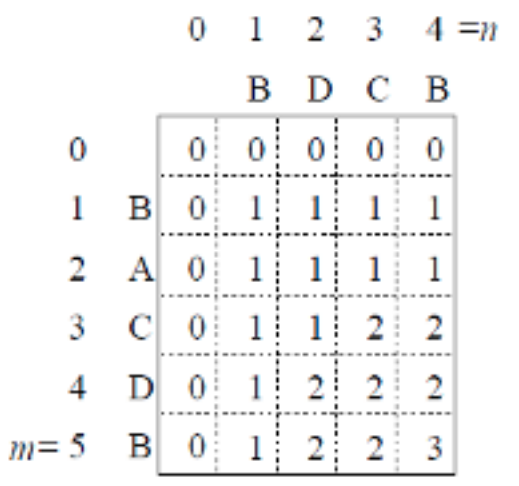
\includegraphics[width =10cm]{LCS-1.png}    
\end{center}
\underline{Step 6:} The value in the last row and the last column is the length of the longest common subsequence.\newline\newline
\underline{Step 7:} If we want to find the longest common subsequence, we start from the last element and follow the direction of the arrow.\newline\newline
\underline{Step 8:} We will do this till we don’t have any pointing arrow left.\newline\newline
The updated table is\newline\newline
\begin{center}
    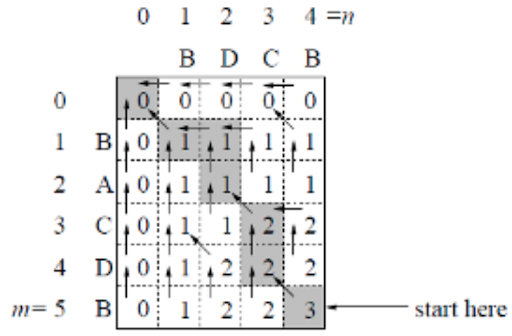
\includegraphics[width =10cm]{LCS-2.png}    
\end{center}
Select the cells where pointing diagonally.\newline\newline
\begin{center}
    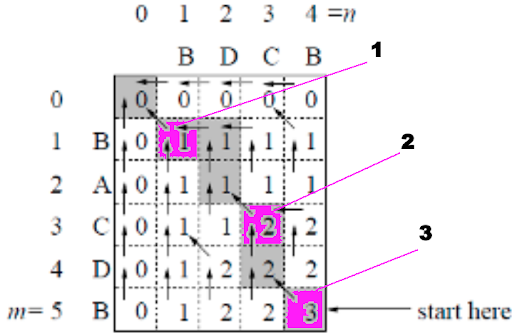
\includegraphics[width =10cm]{LCS-3.png}    
\end{center}
\textbf{Thus the LCS is "BCB".}\newline

Let’s implement it’s pseudo code:-

\begin{lstlisting}
int lcs( char *X, char *Y, int m, int n ) 
{ 
    int L[m + 1][n + 1]; 
    int i, j; 
      
    /* Following steps build L[m+1][n+1] in 
       bottom up fashion. Note that L[i][j] 
       contains length of LCS of X[0..i-1]
       and Y[0..j-1] */
    for (i = 0; i <= m; i++) 
    { 
        for (j = 0; j <= n; j++) 
        { 
        if (i == 0 || j == 0) // base condition if both string are null then answer will be 0
            L[i][j] = 0; 
      
        else if (X[i - 1] == Y[j - 1]) // if character's of both strings are same and we direct count it in answer 
            L[i][j] = L[i - 1][j - 1] + 1; 
      
        else
            L[i][j] = max(L[i - 1][j], L[i][j - 1]); // take maximum of answer after removing one character from both's strings 
        } 
    } 
          
    /* L[m][n] contains length of LCS 
    for X[0..n-1] and Y[0..m-1] */
    return L[m][n]; 
}
\end{lstlisting}

\underline{Time complexity:}\newline
Time complexity of above dynamic programming solution is $O(n \cdot m) + c$, since there is one nested loop for calculating the answer. $c$ is constant which represents the complexity of addition. Taking maximum and return type, assign operations etc..\newline\newline

\underline{Space complexity:}\newline
The space complexity is $O(n \cdot m)$ because we declare a 2 D array of size $n \times m$ and we calculation value for length of $i$ of first string and length $j$ of second string we calculate this answer in $L[i][j]$. Thus we are calculating all values of $n$ and all values of $m$, which translates to filling the whole $L[n][m]$\newline
Thus the complexity is $O(n \cdot m)$.\newline\newline\newline

\section{Longest Repeated Subsequence}

This algorithm finds longest repeating subsequences such that two subsequences don’t have the same string character at the same position.\newline
If any character is repeats then it store in repeated subsequence.\newline
EX. str="aab"\newline
	In this string "a" is repeat\newline

Ex. str="AABEBCDD"\newline
	In this string "ABD" is repeated\newline
We write string two times and compare them with different indexes. If for any character there are present different $i$ and $j$ that miss it is repeated, otherwise not.\\

\underline{Pseudo Code:}\newline

\begin{lstlisting}
string LRP(string str)
{
    int n=str.length();
    int dp[n+1][n+1];
    for (int i=0; i<=n; i++)
        for (int j=0; j<=n; j++)
            dp[i][j] = 0;

    for (int i=1; i<=n; i++)
        for (int j=1; j<=n; j++)
            if (str[i-1] == str[j-1] && i != j)
                dp[i][j] =  1 + dp[i-1][j-1];
            else
                dp[i][j] = max(dp[i][j-1], dp[i-1][j]);
 
// This part of code give longest repeated string

    String res="";
    int i=n,j=n;
    while(i>0 && j>0)
    {
        if(dp[i][j]==dp[i-1][j-1] + 1)
        {
            res+=str[i-1];i--;j--;
        }
        else if(dp[i][j]==dp[i-1][j])
            i--;
        else
            j--;
    }
    reverse(res.begin(),res.end());
    return res;
}

\end{lstlisting}

\underline{Time Complexity:}  $O(n^2)$\newline

\underline{Space Complexity:} $O(n^2)$\\


\section{Count all subsequences having product $< K$}
In this program we have an array or list of numbers. We find all its subsequence and multiply its all numbers . If the product is less than $K$ then we count that subsequence in the answer.\newline

Example: Given $\mathtt{[1,2,3,4]}$ and $K = 10$\newline
Subsequences are\newline
$\mathtt{\{\},\{1\},\{2\}, \{3\}, \{4\}, \{1, 2\}, \{1, 3\}, \{1, 4\}, \{2, 3\}, \{2, 4\},\{3, 4\}, \{1, 2, 3\}, \{1, 2, 4\}, \{2, 3, 4\}, \{1, 2, 3, 4\}}$\newline
The subsequences 
$\mathtt{\{1\},\{2\}, \{3\}, \{4\}, \{1, 2\}, \{1, 3\}, \{1, 4\}, \{2, 3\}, \{2, 4\}, \{1, 2, 3\}, \{1, 2, 4\}}$ satisfy our conditions\newline
So there are 11 subsequences that satisfy our condition. Answer = 11.\\

\underline{Pseudo Code:}\\

\begin{lstlisting}
int productSubSeqCount(vector<int> &arr, int k)
{
    int n = arr.size();
    int dp[k + 1][n + 1];
    memset(dp, 0, sizeof(dp));
  
    for (int i = 1; i <= k; i++) 
    {
        for (int j = 1; j <= n; j++) 
        {
            dp[i][j] = dp[i][j - 1];
            if (arr[j - 1] <= i && arr[j - 1] > 0) 
                dp[i][j] += dp[i/arr[j-1]][j-1] + 1;
        }
    }
    return dp[k][n];
}
\end{lstlisting}

\underline{Time Complexity:} $O(k \cdot n)$.\newline
Space Complexity: $O((k+1) \times (n+1)) \sim O(k \cdot n)$.\\

\section{Edit distance problem}
We have a problem of conversion. Let's take two strings and try to convert one string to another string. Our goal is to find minimum steps or operations to convert a string into another string.\newline
To do that we can apply 'remove' , 'insert', 'replace' operations. Cost of each operation or edit is even.\newline

Example-:\newline
                word1 = "cat"\newline
                word2 = "cut"\newline
We can see that if we convert 'a' into 'u' then both words are the same.\newline

\textbf{\textit{Brute force solution:}}\\

Let's try to think from the basics.\newline
Assume that length's of strings are $m$ and $n$.\\

\textbf{\textit{Recursive solution:-}}\newline
We can start from one end of both strings. If both characters are the same then we leave this and recursively count for remaining parts of both strings. If characters are not the same then we have 3 possibilities to change it.\newline
For this approach insert where we are inserting new character run for $m$ and $n-1$.
For remove operation it will run for $m-1$ and $n$ because we removed one character from the first string. If we replace then obviously recursion would have $m-1$ and $n-1$ length left.\newline
We can take minimum from all 3 answers. Let’s try to figure out the time complexity of the above solution.\\

For every character of the first string we have 3 possibilities. In the worst case time complexity will be $O(3^m)$. So we can’t use it for long strings.\newline
This problem have overlapping subproblems.\\
\begin{center}
    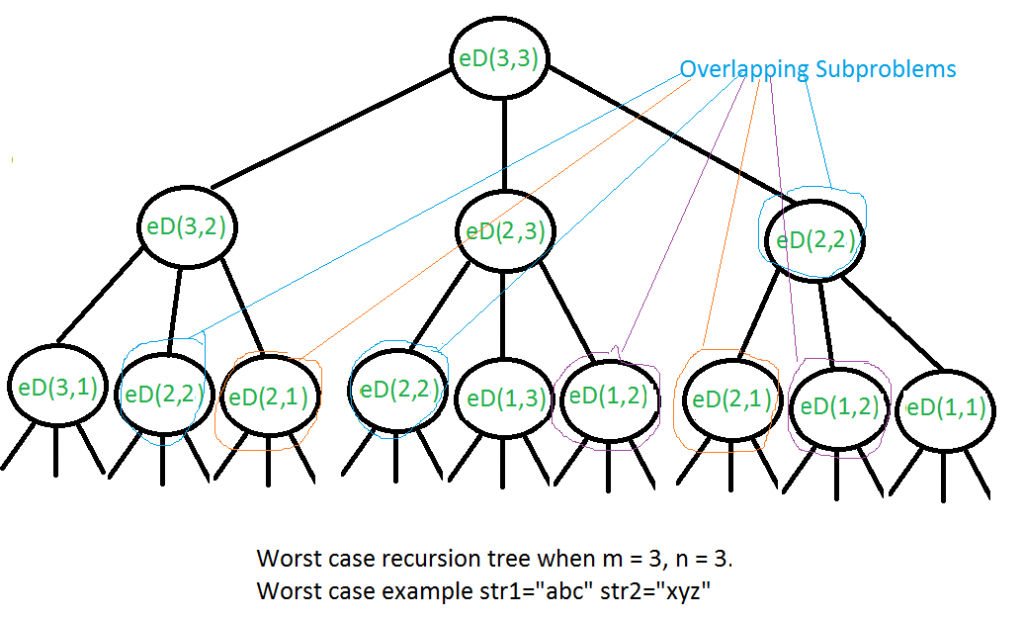
\includegraphics[width = 8cm]{Edit_Distance-1.png}    
\end{center}

We can see in the  above that this problem has many subproblems. Example D(2,2) calculated many times and this problem has optimal substructure.\\

Let’s try to understand how we can use dynamic programming in this.\\
Firstly try to understand base cases:-\\
If the first string is empty then we have to insert all characters in it from the second string.\\
If the second string is empty then we have to remove all characters from it.\\

We had discussed if characters are the same then just ignore them and continue for the rest of the string. If not same then we can take minimum from insert, remove and replace.\\

\underline{Pseudo code-:}\\

\begin{lstlisting}
int editDistDP(string str1, string str2, int m, int n)
{
    // Create a table to store results of subproblems
    int dp[m + 1][n + 1];
    // Fill d[][] in bottom up manner
    for (int i = 0; i <= m; i++) {
        for (int j = 0; j <= n; j++) {
    // If first string is empty, only option is to
    // insert all characters of second string
        if (i == 0)
            dp[i][j] = j; 
    // Min. operations = j
  
/* If second string is empty, only option is to
 remove all characters of second string
 */
            else if (j == 0)
                dp[i][j] = i;
        // Min. operations = i
  
        // If last characters are same, ignore last char
        // and recur for remaining string
            else if (str1[i - 1] == str2[j - 1])
                dp[i][j] = dp[i - 1][j - 1];
 
        // If the last character is different, consider all
        // possibilities and find the minimum
            else
                dp[i][j] = 1 + min(dp[i][j - 1], // Insert
            dp[i - 1][j], // Remove
            dp[i - 1][j - 1]); // Replace
        }
    }
    return dp[m][n];
}
\end{lstlisting}

Time complexity-: easily can be seen from nested loop that it is running for n*m time. Thus time complexity is O(n*m).

Space complexity-: it’s also O(n*m) because we declare a array of n*m size and we are filling it to get the best answer.
Space complexity will be O(n*m).
Now we can solve this problem for big size strings. Mostly upto 1000 (length of strings) and we can see how dynamic programming makes our stuff easy.


\section{Longest palindromic subsequence}
\textbf{\textit{Statement-}}
                 You have given a sequence you have to find the length of longest palindromic subsequence in it.\\

\textbf{\textit{Palindromic-}} 
                 It is a type of word play in which a word spelled forward is the same word spelled backward.\\

\textbf{\textit{Optimal substructure-}} \\
Let us consider the input sequence to be A[0 ... m-1] and B[0 ... n-1] having length $m$ and $n$ respectively. Let $L(A[0 ... m-1], B[0 ... n-1])$ represent the length of the longest common subsequence of two sequence A and B. Now we can state the following recursive definition of $L(A[0 ... m-1], B[0 ... n-1])$ \\
If the last character of both subsequence match ($A[m-1] == B[n-1]$), then\\
\[L(A[0 ... m-1], B[0 ... n-1]) = 1 + L(A[0 ... m-2], B[0 ... n-2])\].\\

If last character of both subsequence are different, then\\
\[L(A[0 ... m-1], B[0 ... n-1]) = MAX(L(A[0 ... m-2], B[0 ... n-1]), L(A[0 ... m-1], B[0 ... n-2])\] \\

\underline{Examples:}\\
Consider two strings A and B such that  A="MUMBAI", B="DELHI".We see that in string A and B their last character is matching so length of their LCS is given by\\
\[L("MUMBAI", "DELHI") = 1 + L("MUMBA", "DELH")\]\\

Consider two strings A and B such that A =”LONDON”, B=”PARIS”, in this case we see their last character is not matching hence the length of their LCS is given by\\
\[L("LONDON", "PARIS") = 1 + MAX(L("LONDO", "PARIS"), L("LONDON", "PARI"))\].\\

\textbf{\textit{Overlapping subproblems-}}\\

Let’s try to implement it.\\
Let assume $arr[0 ... N-1]$ be the input sequence of length $n$ and $L(0, n-1)$ be the length of the longest palindromic subsequence of $arr$.\\
We can see that if last and first characters of $arr$ are same, then \\$L(0, n-1) = L(1, n-2)+2$, otherwise $L(0, n-1) = MAX(L(1, n-1), L(0, n-2)$.\\ \\
\underline{Code:-}
\begin{lstlisting}
int LPS(char *arr , int start , int end)
// declaring the function to calculate lps length
{
/*
Base condition :-
(i) if start and end are equal then answer will be 1;

(ii) if  arr[start] = arr[end] and also start+1 = end then answer will be 2.
*/

if(start == end)
    return 1;

if(arr[start] == arr[end] && start+1 == end)
    return 2;

/* Checking for first and last character-:
If character are same then */

if(arr[start] == arr[end])
    return LPS(arr, start+1, end-1) + 2;

else // if character are not same 
    max(LPS(arr ,start, end-1), LPS(arr, start+1, end));
}
\end{lstlisting}
Let’s try to understand the example "noon"\\

Using code, if the first and last characters of this sequence are equal, then we take the subsequence "oo". Since "oo" is also satisfies the condition, the length of longest palindromic subsequence is 4\\

\underline{Time complexity-} for worst case scenario it will be $O (n^2)$ because for this every time the function will be called.\\

\underline{Space complexity-} the space complexity will be $O(n)$.\\

\section{Longest Increasing Subsequence}
\textbf{\textit{Longest Increasing Subsequence:}}
\newline\newline
The Longest Increasing Subsequence (LIS) problem is to find the length of the longest subsequence of a given sequence such that all elements of the subsequence are sorted in increasing order.\newline 
In this process we find the longest increasing subsequences. Subsequence’s element can be distinct in the original array or can be continuous in the original array. There can be many increasing subsequences. If $i^{th}$ index element is less than all elements whose index less than $i$ then it creates a new subsequence.\newline
Example :\newline
arr[ ] = $\mathtt{\{ 10, 22, 33, 50, 60, 80, 9, 21, 41\}}$\newline
	\textbf{Output: 6}\newline
		There are 2 increasing subsequences $\mathtt{\{ 10, 22, 33, 50, 60, 80\}}$  and $\mathtt{\{9, 21, 41\}}$. So the length of longest increasing subsequence is 6.\newline\newline 
	arr[] = $\mathtt{\{ 3, 10, 2, 1, 20 \}}$\newline
	\textbf{Output: Length of LIS = 3}\newline
	The longest increasing subsequence is $\mathtt{\{ 3, 10, 20\}}$\newline\newline

\textbf{\textit{Method 1 : Recursive}}\newline\newline .
\underline{Optimal Substructure:}\newline
Let $arr[0..n-1]$ be the input array and $L(i)$ be the length of the LIS ending at index $i$ such that $arr[i]$ is the last element of the LIS.\newline
Then, $L(i)$ can be recursively written as : \newline\newline
\begin{center}
$L(i) = 1 + max( L(j) )$ where $0 < j < i$ and $arr[j] < arr[i]$\newline
$L[i] = 1$ , if no such  $j$ exists.\newline\newline
\end{center}
To find the LIS for a given array, we need to return $max(L(i))$ where $0 < i < n$.\newline
Formally, the length of the longest increasing subsequence ending at index $i$, will be 1 greater than the maximum of lengths of all longest increasing subsequences ending at indices before $i$, where $arr[j] < arr[i]$ $(j < i)$. Thus, we see the LIS problem satisfies the optimal substructure property as the main problem can be solved using solutions to subproblems.\newline
This approach is a very time consuming approach. The time Complexity is exponential as there is a case of overlapping subproblem again and again.\newline\newline
\textbf{\textit{Method 2: Dynamic Programming.}}\newline\newline .
In the Recursive method there are many subproblems that are calculated more than one time. By memoization we can avoid recomputation problem.\newline
\underline{Iteration-wise simulation :}
\newline
\begin{center}
$arr[2] > arr[1]$ \{LIS[2] = max(LIS [2], LIS[1]+1) = 2\}\newline\newline
$arr[3] < arr[1]$ {No change}\newline\newline
$arr[3] < arr[2]$ {No change}\newline\newline
$arr[4] > arr[1]$ \{LIS[4] = max(LIS [4], LIS[1]+1) = 2\}\newline\newline
$arr[4] > arr[2]$ \{LIS[4] = max(LIS [4], LIS[2]+1) = 3\}\newline\newline
$arr[4] > arr[3]$ \{LIS[4] = max(LIS [4], LIS[3]+1) = 3\}\newline\newline
\end{center}

\underline{Pseudo Code:}
\begin{lstlisting}
int lis( int arr[], int n ) 
{
 int lis[n];
lis[0] = 1;	
// Compute optimized LIS values in bottom up manner 
 for (int i = 1; i < n; i++ ) 
    	{
        		lis[i] = 1;
        		for (int j = 0; j < i; j++ )  
            		if ( arr[i] > arr[j] && lis[i] < lis[j] + 1) 
                			lis[i] = lis[j] + 1; 
    	}
	int ans=0;
	for(int i=0;i<n;i++)
		ans=max(ans,lis[i]);
	return ans;
}
\end{lstlisting}
\underline{Time Complexity:}
\newline
$O(n \cdot n)+ O(n \cdot log(n))$\newline
$O(N \cdot log(N))$ solution for the LIS problem.
\newline\newline
\underline{Space Complexity:}\newline
$O(n)$
\newline\newline\newline
\section{Longest alternating subsequence:}

\textbf{\textit{What is an alternating sequence?}}\newline
A sequence is called an alternating sequence if its elements satisfy one of the following conditions:\newline
\begin{center}
$x_1 < x_2 > x_3 < x_4 > x_5 ... x_n$\newline
Or\newline
$x_1 > x_2 < x_3 > x_4 < x_5 > ... x_n$\newline
\end{center}

Some examples are\newline
i) Input: arr[ ] = $\mathtt{\{1, 5, 4\}}$\newline
   \textbf{Output : 3}\newline
   (We can see that whole array is of the form $x_1 < x_2 > x_3$, hence length of the longest alternating subsequence is 3)\newline\newline
ii) Input: arr[ ] = $\mathtt{\{1, 4, 5\}}$\newline
   \textbf{Output : 2}\newline
   (We can see all subsequences are of length 2 having the form $x_1 < x_2$ or $x_1 > x2$)\newline\newline
iii) Input: arr[ ] = $\mathtt{\{10, 22, 9, 33, 49, 50, 31, 60\}}$\newline
   \textbf{Output : 6}\newline
   (There are 3 longest subsequences satisfying the condition of alternating subsequence having length 6, these are $\mathtt{\{10,22,9,33,31,60\}}$, $\mathtt{\{10,22,9,49,31,60\}}$, $\mathtt{\{10,22,9,50,31,60\}}$)\newline\newline

This problem is an extension of longest increasing subsequence problem. To solve this problem we create a 2D array $alt[n][2]$ such that $alt[i][0]$ contains longest alternating subsequence ending at index $i$ and in this last element is greater than its previous element whereas $alt[i][1]$ contains longest alternating subsequence ending at index $i$ and last element is smaller than its previous element.\newline
We get the following recursive formulation (optimal substructure property is seen here)\newline
\begin{center}
$alt[i][0] = max(alt[i][0], alt[j][1]+1)$ for all $j < i$ and $arr[j] < arr[i]$\newline\newline
$alt[i][1] = max(alt[i][1], alt[j][0]+1)$ for all $j < i$ and $arr[j] > arr[i]$\newline\newline
\end{center}
The first recurrence relation states that if we are at position $i$ and if this element is bigger than its previous element then for this sequence (upto i) to be bigger we will choose an element ($j < i$) such that $arr[j] < arr[i]$($arr[j]$ can become $arr[i]$’s previous element and if $alt[j][1]+1$ is bigger than $alt[i][0]$ then we will update $alt[i][0]$)\newline\newline
An important point to note that is we have chosen $alt[j][1]+1$ not $alt[j][0]$ because in $alt[j][0]$, the last element is bigger than its previous one and $arr[i]$ is greater than $arr[j]$ which would have broken the alternating property.\newline\newline
Similar things can also be said for the second property.\newline\newline
\underline{Pseudocode:}\newline
\begin{lstlisting}
int main()
{
	int size
	cin>>size
	Int arr[size+1],alt[size+1][2]
	for(int i=0;i<size;i++)
	{
		cin>>arr[i]
	}
	/*Initializing all the values to 1*/
	for(int i=0;i<size;i++)
	{
		alt[i][0]=1
		alt[i][1]=1
	}
	int ans =1 //Initializing the answer
	/* we now compute the values in bottom up manner*/
	for(int i=1;i<size;i++)
	{	
		/* Considering all elements occurring before arr[i]*/
		for(int j=0;j<i;j++)
		{
			/* If arr[i] is greater than arr[j] then,we have to check with alt[j][1]*/
			If (arr[j] < arr[i] && alt[i][0] < alt[j][1] + 1)
			{
				alt[i][0] = alt[j][1] + 1
			}
			/*If arr[i] is smaller than arr[j] then we have to check with alt[j][0]
			If (arr[j] > arr[i] && alt[i][1] < alt[ij[0] + 1)
			{
				alt[i][0] = alt[j][1] + 1
			}
		/* we now select the maximum value among all index i */
	if( ans < max(alt[i][0].alt[i][1])
	{
		ans = max(alt[i][0].alt[i][1]
	}
}
cout<<ans<<'\n';
return 0
}
\end{lstlisting}
\underline{Time complexity:}\newline
We see that two nested loop is being used therefore time complexity is $O(n^2)$\newline\newline
\underline{Space complexity:}\newline
Due to usage of arrays,space complexity is $O(n)$\newline

\chapter{Rod Cutting Problem}

\textbf{\textit{Optimal substructure-}} shreyansh you have to do it.\\

\textbf{\textit{Statement-}}
Given a rod of length $n$ inches and an array of prices that contains prices of all pieces of size smaller than $n$. Determine the maximum value obtainable by cutting up the rod and selling the pieces.
Let’s try to understand it with example \\

Let assume the length of rod is 8 and prices are followings-:\\

\begin{center}
\begin{tabular}{ | m{1.5cm} | m{1cm}| m{1cm} | m{1cm} | m{1cm} | m{1cm} | m{1cm} | m{1cm} | m{1cm} | } 
\hline
Length & 1 & 2 & 3 & 4 & 5 & 6 & 7 & 8  \\ 
\hline
Price & 3 & 5 & 8 & 9 & 10 & 17 & 17 & 20  \\
\hline
\end{tabular}
\end{center}


You can easily see that if we cut it in 8 parts, then obtained value is 24, which is the maximum.\\

\textbf{\textit{Overlapping subproblem-}}\\

\begin{lstlisting}
int cutrod(int *price, int n) // declaration of function
{
//Base condition-:
if(n <= 0)
    return 0;   // no pice left
int val[n+1];
val[0] = 0;   //base declaration
for(int i=0; i<n; i++)
{
    // iterate over length of rod
    max_value = infinity
    for(int j=0; j<i ; j++)
    {
        max_value = MAX(max_value, price[i] + val[i-j-1]);
            //Taking the maximum obtained price.
    }
    val[i] = max_value;r
    return max_value;
}
\end{lstlisting}

\underline{Time complexity-} the time complexity of this is $O(n^2)$\\

\underline{Space complexity-} $O(n)$ because we declare one array to store values.\\

\chapter{Prefix Sum Using Dynamic Programming}
It is one of the most fundamental concepts used in solving various problems in competitive programming and it is also used in various algorithms.\\
\underline{Prefix sum:} Given an array arr[ ] of size $n$, its prefix sum is another array (lets call it prefsum[ ]) of same size $n$. Here the value of prefsum at a particular index is the sum of given array till that index\\

\[(pref[i] = arr[1] + arr[2] + ...  + arr[i])\]\\

\underline{Pseudo code:}\\
\begin{lstlisting}
int main()
{
    int arr[n],prefsum[n]
	// n is size of the given array,
    pref[0]=arr[0];
	//setting initial element of prefsum
    for(int i=1; i<n; i++)
    {
        prefsum[i] = prefsum[i-1]+ arr[i];
    }
    for(int i=0; i<n; i++)
    {
        cout<<arr[i]<<" ";
    }
}
\end{lstlisting}

\underline{Time complexity:}\\
We see that loop runs through $n$ iterations,Hence time complexity is of order $O(n)$.\\

\underline{Space complexity:}\\
Space complexity of order $O(n)$ as we are using an array of size $n$.\\

\chapter{Matrix Chain Multiplication Algorithm}
In matrix chain multiplication problem, we are provided with a sequence of matrices and our goal is to find the most efficient way to multiply these matrices.\\
We know that matrix multiplication is associative (i.e no matter how we parenthesize the product the result will be same).\\
Since matrix multiplication is associative our main goal is to decide the sequence of matrix multiplications involved. For example if there are four matrices A, B, C and D then we will have the following orders of multiplication of matrices.\\
\[((A\times B)\times C)\times  D=(A\times (B\times C))\times  D=(A\times  B) \times (C\times  D)=A\times ((B\times  C)\times  D)=A\times  (B\times (C\times  D))\]\\
The order in which product is parenthesized affects the number of of simple arithmetic operations needed to compute the product, i.e., the efficiency.\\
Suppose A is a $10\times 30$ matrix, B is a $30\times 5$ matrix and C is a $5\times 60$ matrix. Then the number of operations are -\\ 
\begin{align*}
    (A\times  B)\times  C &= (10\times  30\times  5) + (10\times  5\times  60)=1500 + 3000 = 4500\\
     A\times  (B\times  C) &= (30\times  5\times  60) + (10\times  30\times  60) = 9000 + 18000 = 27000\\
\end{align*}

We see that first parenthesization requires less number of operations.\\
If there are two matrices then the only way to know the minimum cost of operations is by multiplying them.\\    In general, the following recursive algorithm can be used to find the minimum cost.
    1) Take the sequence of matrices and separate it into two subsequences.\\
    2) Find the minimum cost of multiplying each subsequence.\\
    3) Add these costs together,and add the cost of multiplying two result matrices.\\
    4) Do this for each possible position at which the sequence of matrices can be split, and take the minimum over all of them.\\

Now we observe optimal substructure and overlapping subproblems property in this problem and construct to show that it can be solved using dynamic programming.\\

\textbf{\textit{i) Optimal Substructure:}}\\
  For example if we take four matrices A, B, C, D, we compute the cost required to find all possible parenthesize combination that is $(A)\times (B\times C\times D), (A\times B)\times (C\times D), (A\times B\times C)\times (D)$,we make recursive calls to find the minimum cost to compute $(A\times B\times C), (A\times B) ,(C\times D)$ and $(B\times C\times D)$ and we choose the best one. From above procedure stated in recursive algorithm, we see that this follows optimal substructure properties.\\

\textbf{\textit{ii) Overlapping subproblems:}}\\
    We see that in optimal substructure property in the recursive algorithm described above we are performing a lot of redundant works. For example we are making recursive calls for finding the best cost for computing both $(A\times B\times C)$ and $(A\times B)$. But finding the best cost for computing $(A\times B\times C)$ also requires finding the best cost of $(A\times B)$. Hence many repetition of this type occurs that are unnecessary.\\
The algorithm represented above is a naive approach and since it is a recursive algorithm its time complexity is of exponential form which is quite slow. We now represent a more efficient dynamic programming solution using memoization.\\

\underline{Pseudocode:}\\
\begin{lstlisting}
MatrixChainOder(int dims[])
    /* Matrix A[i] has dimensions dims[i-1] x dims[i] for i=1 ... n */
{
	n = dims.length-1;  // length[dims] = n+1
    /* m[i,j] = Minimum number of scalar multiplications (i.e., cost) */
    /* needed to compute the matrix A[i]A[i+1]...A[j] = A[i...j]
       The cost is zero when multiplying one matrix */

    for (i = 1; i <= n; i++)
    {	
        m[i, i]=0;
    }
    for(len = 2; len <= n; len++)
    {
        //subsequence lengths
        for(i = 1; i <= n-len+1; i++)
        {
            j = i+len-1;
            m[i ,j] = MAXINT;
            for(k = i; k <= j-i; k++)
		{	
                cost = m[i, k] + m[k+1, j] + dims[i-1]*dims[k]*dims[j];
                if(cost <m[i, j])
                {
                    m[i, j] = cost;
                    s[i, j] = k;
        /* index of the subsequence split that achieved the minimal cost */
                }
           }
        }
    }
}
\end{lstlisting}
\underline{Time complexity: } Above algorithm is using three nested for loops, hence time complexity is $O(n^3)$. We see that this is much faster than the naive recursion approach.\\

\chapter{Coin Change Problem}	
\textbf{\textit{Problem statement:}}\\
Given a value N, if we want to make the change for N cents, and we have infinite supply of each of S = \{$S_1, S_2, ..., S_m$\} valued coins, in how many ways can we make the change? Order of coins doesn’t matter.\\

Examples:\\

i) If we have N=4 and S=\{$\mathtt{1, 2, 3}$\}\\
In this case there are four solutions $\mathtt{\{1, 1, 1, 1\}, \{1, 1, 2\}, \{2, 2\}, \{1, 3\}}$\\
Therefore the output is 4.\\

ii) If we have N=10 and S = $\mathtt{\{2, 5, 3, 6\}}$\\
In this case there are five solutions $\mathtt{\{2, 2, 2, 2, 2\}, \{2, 2, 3, 3\}, \{2, 2, 6\}, \{2, 3, 5\}, \{5, 5\}}$\\
Therefore the output is 5.\\

Let us examine optimal substructure and overlapping subproblems in this question.\\

\textbf{\textit{Optimal substructure:}}\\
To count the total number of solutions, all sets of solutions can be divided into two sets.\\
First set contains solutions that do not contain $m^{th}$ coin (or $S_m$)\\
Second set contains solutions that contain atleast one $S_m$.\\
Let $count(S[$  $] ,m, n)$ be the function to count the number of solutions, therefore we can write it as sum of $count(S[$ $], m-1, n)$ and $count(S[$ $], m, n-S_m)$.
From the above concept, we see that the problem is having optimal substructure property as it is solved using the solution of its subproblems.\\

\textbf{\textit{Overlapping subproblems:}}\\
Following is the pseudo code for simple recursive solution of the coin change problem.\\

\begin{lstlisting}
/* Below function returns the count of ways
    we can sum S[0...m-1] coins to get sum n. */
int count(int s[ ], int m, int n)
{
    // if n is 0 then there is 1 solution (do not include any coin)
    if (n == 0)
        return 1;
    // If n is less than 0 then no solution will exist
    if ( n < 0)
        return 0;
    // If there are no coins and n is greater than 9,
	then no solution exists */
    if (m <= 0 && n >= 1)
        return 0;
    // count is sum of solutions (i) including s[m-1]
    // (ii) Excluding s[m-1]
    return count(S, m-1, n) + count(S, m, n-s[m-1]);
}
int main()
{
    int i,j;
    int arr[];
    int m; // length 
    for (int i=0; i < m; i++)
    {
        cin>>arr[i];
    }
    int n;
    cin>>n; \\Given value n
    cout<<cout(arr, m, n);
}
\end{lstlisting}

We see that there are a lot of parts that are calculated multiple times hence it results in overlapping subproblems. This naive method is of exponential time complexity.\\

We now look at the dynamic programming solution. Below is the given pseudocode.\\

\begin{lstlisting}
int count(int S[], int m, int n)
{
    int i, j, x, y;
/* We need n+1 rows as the table is constructed 
in bottom up manner using the base case 0 */
// Value case (n=0)
    int table[n+1][m];
//Fill the entries for 0
//value case (n=0)
    for(i = 0; i < m; i++)
    {
        table[0][i]=1;
    }
// Fill reset of the table entries in bottom up manner
    for (int i=1; i < n; i++)
    {
        for(int j=0; j < m; j++)
        {
        //count of solutions including S[j]
            x = (i-s[j] >= 0) ? table[i-s[j]][j] : 0;
        //count of solutions excluding S[j]
            y = (j>=1) ? table[i][j-1] : 0;
        //total count
            table[i][j] = x + y;
        }
    }
    return table[n][m-1];
}
int main()
{
    int arr[] ={};
    int m; //length of array arr.
    int N; // Given value N
    for(i = 0 ; i < m; i++)
    {
        cin>>arr[i];
    }
    cout << count(arr,m,n);
    return 0;
}
\end{lstlisting}
\underline{Time complexity:} 
We see that two nested for loops are being used therefore time complexity is $O(m \cdot n)$\\

\underline{Space complexity:} 
Space complexity is also of order $O(m \cdot n)$.\\

\chapter{Floyd Warshall algorithm}
\textbf{\textit{Introduction:}}\\
Floyd-Warshall Algorithm is an algorithm for finding the shortest path between all the pairs of vertices in a weighted graph. This algorithm works for both the directed and undirected weighted graphs. However, it does not work for the graphs with negative cycles (where the sum of the edges in a cycle is negative). This algorithm follows the dynamic programming approach to find the shortest paths.\\
\textbf{\textit{Algorithm:}}\\
\textit{Description of algorithm:}\\
The main idea of this algorithm is to divide the process of finding the shortest path between any two vertices to several incremental phases.\\

Let us consider vertices starting from 1 to $n$. Let the matrix storing distance between two vertices be \textit{dis[ ][ ]}.\\
Before $k^{th}$ phase \textit{(k = 1 ... n) d[i][j]} stores the minimum distance found from intermediate vertices from the set $\mathtt{\{1, 2, 3 ... k-1\}}$.\\

We can say that before $k^{th}$ phase value of $d[i][j]$ corresponds to the shortest path from vertex $i$ to vertex $j$ if we are allowed to go only through the intermediate vertices from the set $\mathtt{\{1, 2, 3 ... k-1\}}$.\\
We initially set distance between any vertex $i$ and $j$ as infinite (i.e $dis[i][j] = \infty$) if there is no edge in between $i$ and $j$.\\
If there is an edge between $i$ and $j$, then we set $d[i][j] = w_{ij}$ ($w_{ij}$ is the weight of the edge given between $i$ and $j$), also we set distance between same vertices as 0.\\

Now suppose we are in $k^{th}$ phase and we want to compute the matrix \textit{dis[ ][ ]}. We have to fix the distances for some vertices pairs $(i, j)$. There are two fundamentally different cases:\\
    1) The shortest way from the vertex $i$ to the vertex $j$ with internal vertices from the set $\mathtt{\{1, 2, 3 ... k\}}$ coincides with the shortest path with the internal vertices from the set $\mathtt{\{1, 2, 3 ... k-1\}}$\\
 In this case, $dis[i][j]$ will not change during the transition.\\
    2) The shortest path with internal vertices from {1,2,...,k} is shorter.\\

This means that the new shorter path passes through the vertex $k$. This means that we can split the shortest path between $i$ and$j$ into two paths: the path between $i$ and $k$, and the path between $k$ and $j$. It is clear that both this paths only use internal vertices of $\mathtt{\{1, 2, 3 ... k-1\}}$ and are the shortest such paths in that respect. Therefore we already have computed lengths of those paths before, and we can compute the length of the shortest path between $i$ and $j$ as $dis[i][k] + dis[k][j]$.\\

Combining these two cases we find that we can recalculate the length of all pairs $(i,j)$ in the $k_{th}$ phase in the following way:\\
\textbf{\[dis[i][j] = min(dis[i][j], dis[i][k] + dis[k][j]).\]}\\

\underline{Pseudo Code:}\\

\begin{lstlisting}
/* Create a |n| x |n| matrix dis that will
    describe the distances between vertices */

For each cell (i, j) in dis:
    if i == j:
        dis[i][j] = 0
    if (i, j) is an edge in graph:
        dis[i][j] = weight(i,j)
    else:
        dis[i][j] = infinity
        for k from 1 to |n|:
            for i from 1 to |n|:
                for j from 1 to |n|:
                    if dis[i][j] > dis[i][k] + dis[k][j]
                        dis[i][j] = dis[i][k] + dis[k][j]
\end{lstlisting}

\underline{Time complexity:} \\
We see that in the above pseudocode three nested loops are being used therefore the time complexity is $O(n^3)$.\\

\underline{Space Complexity:}\\
We see that we are using a 2-D array to store distance between two vertices, therefore space complexity is $O(n^2)$.\\

\textbf{\textit{How to identify negative cycle:}}\\
Run Floyd-Warshall algorithm on the graph, initially $dis[v][v] = 0$ for each $v$. But after running the algorithm, $d[v][v]$ will become smaller than 0 if there exists a negative length path from $v$ to $v$. We can use this to also find all pairs of vertices that don’t have a shortest path between them.\\

\textbf{\textit{Proof of the algorithm:}}\\
(To be done by Manoj)\\

\chapter{Subset Sum Problem}

\textbf{\textit{Problem statement:}}\\
Given a set of non-negative integers, and a value sum, determine if there is a subset of the given set with sum equal to given sum.\\

\underline{Example 1:}\\

Input: set[ ] = \{$\mathtt{3, 34, 4, 12, 5, 2}$\}, sum = 9\\
\textbf{    Output: True}\\

There exists a subset \{$\mathtt{3, 4}$\} in the above set whose sum is 9.\\

\underline{Example 2:}\\

Input: set[ ] = \{$\mathtt{3, 34, 4, 12, 5, 2}$\}, sum = 30\\
\textbf{    Output: False}\\

There is no subset of the above set whose sum is 30.\\

We first see a naive recursive approach to solve this problem and then an efficient dynamic programming solution.\\

\textbf{\textit{Recursive Approach:}}\\
Let the target sum equal to the given sum we need to obtain.\\

In the recursive approach we consider two cases:\\
We consider the last element present in main set in our subset as a result\\
\textit{required sum = target sum - value of last element and number of element = total elements - 1.}\\

Leave the last element. Now,\\
\textit{required sum = target sum and total number of elements = total elements - 1.}\\

Therefore we get the following recursive formula for Subsetsum() problem\\
\textit{Subsetsum(set, n, sum) = Subsetsum(set, n-1, sum)} $\mid\mid$ \textit{Subsetsum(set, n-1, sum-set[n-1])}\\

We will have the following base cases:\\
\begin{align*}
\textit{Subsetsum(set, n-1, sum)} &= \textit{false if sum $>$ 0 and n == 0}\\
\textit{Subsetsum(set, n, sum)} &= \textit{true if sum == 0}\\
\end{align*}

Let us look at the simulation of the above recursive problem\\
\begin{align*}
set[ ] &= \{3,4,5,2\} \\
Target sum &= 9\\
\end{align*}

Let (x, y) = 'x' is the number of elements left and 'y' is the required sum.\\\\

\Tree[.(4,9)\\True [.(3,6) [.(2,2)\\True [.(1,-3)\\False ] [.(1,2)\\True [.(0,0)\\True ]
               [.(0,2)\\False ]] ]
               [.(2,6) ]]
          [.(3,9) [.(2,5) ]
                [.(2,9) ]]]\\\\



\underline{Pseudocode for recursive approach:}\\

\begin{lstlisting}
/*This function returns true if there is a subset of
 set set[ ] with sum equal to the given sum. */

bool Subsetsum(int set[ ], int n, int sum)
{
    //Following 2 if's are base cases
    if (sum == 0 )
    {
        return true;
    }
    if (n == 0)
        return false;
  /*This condition checks whether the last element
 is greater than sum, if condition is true
         then ignore the element */

    if (set[n-1] > sum)
        return Subsetsum(set, n-1, sum);

/*Else we check if sum can be obtained
         by any of the following
    (a) including the last element
    (b) excluding the last element
*/
    return Subsetsum(set, n-1, sum) || Subsetsum(set, n-1, sum-set[n-1])
}
int main()
{
    int size, sum;
    cin>>size>>sum;
    int set[size+1];
    for (i = 0; i < size; i++)
    {
        cin>>set[i];
    }
    if (Subsetsum(set, size, sum) == true)
    {
        cout<<"Subset exists";
    }
    else
    {
        cout<<"Subset doesn't exist";
    }
    return 0;
}
\end{lstlisting}

\underline{Time complexity of recursive approach:}\\
We see that the above approach may try all subsets of the given set in the worst case. So it is of exponential complexity.\\
In fact this is NP-complete (There is no known polynomial time solution for this problem)\\

We now see a much efficient approach using dynamic programming.\\
In dynamic programming approach we create a 2D array of size $(arr.size()+1) \times (target+1)$ of data type boolean. The state dp[i][j] will be true if there exists a subset of elements from A[0 ... i] with sum value = j.\\

Following is the approach of this problem using dynamic programming:\\
\begin{lstlisting}
if (A[i] > j )
    dp[i][j] = dp[i-1][j];
else
    dp[i][j] = dp[i-1][j] or dp[i-1][j-a[i]];
\end{lstlisting}

The meaning of the above approach is that if value of the last element A[i] is greater than the current sum, then we ignore A[i] and copy the answer from the previous case. If the current value is greater than the $i^{th}$ element, we will see if any of the previous states have already experienced $sum=j$, we can think in terms of if dp[i-1][j-A[i]] is true then we can include current element in subset so that sum equals j or if there is already a subset with sum j,we can include it here.\\

We can look at the simulation of this approach\\
\[Set[] = \mathtt{\{3, 4, 5, 2\}}\]
\[Target sum = 6\]\\

\begin{center}
\begin{tabular}{ | m{1cm} | m{1cm}| m{1cm} | m{1cm} | m{1cm} | m{1cm} | m{1cm} | m{1cm} | } 
\hline
  & 0 & 1 & 2 & 3 & 4 & 5 & 6  \\ 
\hline
0 & T & F & F & F & F & F & F  \\
\hline
3 & T & F & F & T & F & F & F \\
\hline
4 & T & F & F & T & T & F & F \\
\hline
5 & T & F & F & T & T & T & F\\
\hline
2 & T & F & T & T & T & T & T\\
\hline
\end{tabular}
\\
\end{center}

\underline{Pseudocode of the above approach:}\\

\begin{lstlisting}
/* Returns true if there exists a subset of set[ ]
   with sum equal to the given sum
*/
bool Subsetsum(int set[ ], int n, int sum)
{
/* The value of subset[i][j] will be true
if there is a subset of set[0..j-1] 
with sum equal to i */

    bool subset[n+1][sum+1];
// if sum is 0, then answer is true
    for(i = 0; i <= n; i++)
    {
        subset[i][0] = true;
    } 
/* On the other hand if sum is not
and set is empty, then answer is false

We now fill the subset table in bottom up manner
*/
    for(i = 1; i <= n; i++)
    {
        for(j = 1; j <= sum; j++)
        {
            if(j < set[i-1])
            {
                subset[i][j] = subset[i-1][j];
            }
            if (j >= set[i-1])
                {
                    subset[i][j] =
            subset[i-1][j] || subset[i-1][j-set[i-1]];
                }
        }
    }
    return subset[n][sum];
}

int main()
{	
    int size, sum, set;
    cin>>size;
    cin>>sum;
    int set[size+1];
    for(i = 0; i < size; i++)
    {
        cin>>set[i];
    }
    if(Subsetsum(set, n, sum) == true)
    {
        cout<<"Subset with the given sum exists";
    }
    else
    {
        cout<<"Subset with the given sum does not exist";
    }
    return 0;
}
\end{lstlisting}

\underline{Time Complexity:}\\
Since we are using two nested loops, time complexity is $O(sum \times n)$\\
Here $sum$ is the target sum and $n$ is the size of the array.\\

\underline{Space Complexity:}\\
Here we are using a 2-D array and its size is $sum \times n$.\\
Therefore space complexity is $O(sum \times n)$

\chapter{Partition Problem}

\textbf{\textit{Problem statement:}}\\
This problem is used to determine whether a set can be partitioned in two subsets having sum in both subsets same.\newline
To solve this problem we can think of two main steps that can be used. These are:-\newline
i) Calculate total sum of all elements in the array, If it is odd then it can never be divided in two parts.\newline
ii) If the sum is even then we have to find a subset having sum equal to (total sum/2),if it exists then our solution exists.\newline\newline
We first see the naive recursive solution and then we will look up on much efficient dynamic programming solution.\newline\newline
\textbf{\textit{Recursive Solution:}}\newline\newline
We see the following recursive property:\newline
Let Subsum(arr,n,sum/2) be a function that returns true when a subset of an array arr[0...n-1] exists with sum equal to sum/2.\newline
This Subsum function can be divided further into two problems\newline
i) Subsum without having the last element(in this case n reduces to n-1)
ii) Subsum which is having the last element(Here sum/2 reduces by arr[n-1] (since we need to find total sum as sum/2 and we have included arr[n-1], so remaining is sum/2-arr[n-1], also n changes to n-1 as we are moving to other element)\newline
Therefore if any of the above two subproblems are true then it returns true.\newline
Hence above recursive function can be written as\newline
Subsum(arr,n,sum/2) = Subsum(arr,n-1,sum/2) $\mid\mid$ Subsum(arr,n-1,sum/2-arr[n-1])\newline\newline
\textbf{\textit{Implementation of recursive solution:}}\newline

\begin{lstlisting}
bool Subsum(int arr[],int size, int sum)
{
    //These are base cases
    if (sum==0)
    {
        return true;
    }
    if (n==0 && sum!=0)
    {
        return false;
//since subset sum cannot exist
    }
//If last element is greater than the sum,we ignore it
    if (arr[n-1] > sum)
        return Subsum(arr,n-1,sum);
/* Else sum can be obtained from either of following two ways
i) Including last element
ii) Excluding last element/*
    return
    Subsum(arr,n-1,sum)||Subsum(arr,n-1,sum-arr[n-1]);
}
int main()
{
    int size,sum=0;
    cin>>size;
    int arr[size+5];
    for(int i=0;i<size;i++)
    {
        cin>>arr[i];
        sum+=arr[i];
//calculating the total sum
	}
    if (sum%2!=0)
    {
        cout<<''Cannot be divided into two subsets"; //since   total sum is odd
    }
    else
    {
        if(Subsum(arr,n,sum/2)==true)
        {
            cout<<''Set can be divided in two subsets'';
        }
        else
	    {
		    cout<<''Set cannot be divided in two subsets'';
	    }
	}
    return 0;
}
\end{lstlisting}

We see since it is a recursive algorithm it is having exponential time complexity. We now look at the much faster dynamic programming approach.\newline\newline

\textbf{\textit{Dynamic Programming approach}}\newline\newline

\begin{lstlisting}
int partition (int arr[],int sum,int size)
{
    bool partit[sum/2+1][size+1];
//we set up the base cases
    for(int i=0;i<=size;i++)
    {
        partit[0][i]=true;
    }
    for(int i=1;i<=sum/2;i++)
    {
        partit[i][j]=false;
/*since sum=0 and size!=0 returns false/*
    }
    for(int i=1;i<=sum/2;i++)
    {
        for(int j=1;j<=size;j++)
        {
            if(i>=arr[j-1])
            {
                partit[i][j]=
                partit[i][j-1]||partit[i-arr[j-1]][j-1];
            
/* if arr[j-1] is smaller than the required
sum i,we check cases of including
and excluding last element/*

            }
            else
            {
                partit[i][j]=
                partit[i][j-1];
/*if arr[j-1] is greater than sum
we simply ignore it/*

            }
        }
    }
    return partit[sum/2][size];
}

int main ()
{
    int size,sum=0;
    cin>>size;
    int arr[size+5];
    for(int i=0;i<size;i++)
    {
        cin>>arr[i];
        sum+=arr[i];
//calculating the total sum
    }
    if (sum%2!=0)
    {
        cout<<''Can not be divided into two subsets''; //since   total sum is odd
    }
    else
    {
        if(partition(arr,sum,size)==1)
        {
            cout<<''Can be divided into two subsets'';
        }
        else
        {
            cout<<''Cannot be divided into two subsets'';
		}
    }
    return 0;
}
\end{lstlisting}

\underline{Time complexity:}\newline
From above algorithm there is a nested loop, so time complexity is $O(sum \times size)$
\newline\newline
\underline{Space complexity:}\newline
Due to 2d array, space complexity is also $O(sum \times size)$\newline

\chapter{Longest Bitonic Subsequence Algorithm}

\textbf{\textit{What is a bitonic subsequence?}}\newline
Given any array $arr[0...n-1]$ containing $n$ integers, a subsequence of $arr$[ ] is called bitonic if it is first increasing ,then decreasing.\newline
A sequence which is sorted in increasing order is considered bitonic with decreasing part empty. Similarly a decreasing sequence is considered as bitonic with increasing part as empty.\newline\newline
Following are some examples;\newline\newline
i) Input arr[ ] = $\mathtt{\{1, 11, 2, 10, 4, 5, 2, 1\}}$\newline
   \textbf{Output: 6}\newline
   (Longest Bitonic Subsequence is (1, 2, 10, 4, 2, 1) having length 6)\newline\newline
ii) Input arr[ ] = $\mathtt{\{12, 11, 40, 5, 3, 1\}}$\newline
   \textbf{Output: 5}\newline
   (Longest Bitonic Subsequence is (12,11,5,3,1) having length 6)\newline\newline
iii) Input arr[ ] = $\mathtt{\{80, 60, 30, 40, 20, 10\}}$\newline
   \textbf{Output: 5}\newline
   (Longest Bitonic Subsequence is (80,60,30,20,10) having length 6)\newline\newline

This problem is like an extension of longest increasing subsequence problem discussed in this book. Suppose we are given array $arr$[ ] and its length $n$ as input. We have to construct two arrays $forw$[ ] and $backw$[ ] using dynamic programming solution of LIS problem. $forw[i]$ stores the length of the longest increasing subsequence ending with $arr[i]$ while $backw[i]$ stores the length of the longest decreasing subsequence starting with $arr[i]$. Finally we will have to return the maximum value of $forw[i] + bacw[i] - 1$\newline\newline
\underline{Pseudocode of the algorithm:}\newline\newline
\begin{lstlisting}
Int main()
{
	Int size
	cin>>size
	Int arr[size+5],forw[size+5],backw[size+5]
	for(int i=0;i<size;i++)
	{
		cin>>arr[i]
	}
	//initializing initial length as 1
	for(int i=0;i<size;i++)
	{
		forw[i]=1   
		backw[i]=1
	}
	//We are now computing LIS from left to right
	for(int i=1;i<size;i++)
	{
		for(int j=0;j<i;j++)
		{
			If (arr[i] > arr[j] && forw[i] < forw[j]+1)
			{
				forw[i]=forw[j]+1
			}
		 }
	}
//We are now computing LDS from right to left
for(int i=size-2;i>=0;i--)
	{
		for(int j=size-1;j>i;j--)
		{
			If (arr[i] > arr[j] && backw[i] < backw[j]+1)
			{
				backw[i]=backw[j]+1
			}
		 }
	}
	//We now compute maximum value of forw[i]+back[i]-1
	int maxim = forw[i] + backw[i] -1
for(int i=1;i<size;i++)
{
	if(forw[i]+backw[i]-1>maxim)
	{
		maxim = forw[i] + backw[i]-1
	}
}
	cout<<maxim<<'\n';
	return 0
}
\end{lstlisting}

\underline{Time complexity:}\newline
We see that due to  two nested loops time complexity is $O(n^2)$\newline\newline
\underline{Space complexity:}\newline
Due to presence of arrays space complexity is $O(n)$\newline\newline

\chapter{Dynamic Programming in Combinatorics}

\section{Compute $\mathbf{n \choose r}$ \textbf{\% p}}
If value of $n \choose r$ is small then we directly compute $n \choose r$ \% p.\\

What if the value of $n \choose r$ is large?\\

In this case the value of $n \choose r$ can not fit in a variable cause of overflow. For this problem we have to use a special approach which is divide and conquer.\\

\underline{Pseudo Code:}\\

\begin{lstlisting}
int nCrmodp(int n, int r, int p)
{
    if(r > n-r)
    r = n-r;
    int c[r+1];
    memset(c, 0, sizeof(c));
    c[0] = 1;

    for(int i = 1; i <= n; i++)
    {
        for(int j = min(i, r); j > 0; j--)
        {
            c[j] = (c[j] + c[j-1]) % p;
        }
    }
    return c[r];
}
\end{lstlisting}

\textbf{\textit{Explanation of code:}}\\
\begin{center}
$ {n \choose r} = {n \choose n - r} $\\
\end{center}

We want a minimum calculation so we take the value of $r$ as min(r, n-r).// 
First declare an array size of $r+1$ and set to 0. Now set c[0] = 1. We create a loop which is running $n$ times. In each loop we update the value of the array from $j$ = $min(i, r)$ to $j = 1$. We just add previous value at each position also take modular when we add the value. After completing the loop we just return the value which is at $r^{th}$ place.\\

This return value is $n \choose r \% p $.\\

\underline{Time Complexity:} 
We run the first loop $n$ times and second loop $min(i, r)$ times. If we take the worst case then $min(i, r)$’s value is $r$. So time complexity is $n \cdot r$\\.
Time complexity = $O(n \cdot r)$.\\

\underline{Space Complexity:}
We declare an array size of $(r+1)$ and $r$ is $min(r, n-r)$. In any condition $r$ will always be less than or equal to $\frac{n}{2}$. So Space complexity is $O(\frac{n}{2})$. On rounding it is $O(n)$.\\

\underline{Space Complexity:}
    $O(n)$.\\

\section{Lobb Number:}
The LOBB NUMBER $L(m, n)$ counts the number of ways that $n+m$ open parentheses can be arranged to form the start of a valid sequence of balanced parentheses.\\

The LOBB NUMBER are parameterized by two-negative $m$ and $n$ ($n>=0 \&\& m>=0$). The formula for this is\\
\[L(m, n) = \frac{2m + 1}{m + n + 1} \cdot {2n \choose m + n}\]\\

LOBB number is also used to count the number the ways in which n+m copies of the value +1 and n-m copies of the value -1 may be arranged into a sequence such that all of the partial sums of the sequence are non-negative.\\
To calculate the LOBB number we have to calculate the binomial coefficient which can represented as $c(n, k)$ same as we did ${n \choose r} \% p$ in previous example.\\

\section{Number of solution of linear equation}
\textbf{\textit{Statement:}}\\
Given a linear equation of $n$ variables, we have to find a number of non-negative solutions of this equation.\\

Let’s try to understand the naive solution for this example.\\
We simply run a loop for all $n$ variables and check that it can be a solution for this or not.\\
The time complexity of this solution is exponential and we can't solve it for larger value of $n$.\\

We can solve this problem using dynamic programming.  $coff$ arr is the array where it store the cofficient of equation.\\

\underline{Pseudo code:-}\\
 \begin{lstlisting}
int dp[rhs+10] ={0};
/* declaring the dp array where 'rhs' is
  right side number of linear equation.
*/
dp[0] = 1;
for(int i = 0; i < n; i++)
for(int j = coff[i]; j <= rhs; j++)
    dp[j] += dp[j-coff[i]];
\end{lstlisting}

Number of solution is dp[rhs]\\

\underline{Time complexity:} The complexity of above solution is $O(n \times rhs)$\\

\underline{Space complexity:-} $O(n)$\\


\section{Eulerian Number}
Eulerian number $A(n, m)$ is the number of permutations of the numbers 1 to $n$ in which exactly $m$ elements are greater than the previous element (permutations with $m$ "ascents").\\

Example:    Take $n = 3 , m = \mathtt{\{0, 1, 2\}}$, total permutations = 3! = 6\\

\begin{center}
\begin{tabular}{ | m{2.5cm} | m{2.5cm}| m{2cm} | } 
\hline
Permutation  & Instance & Count \\ 
\hline
1 2 3 & 1, 2 \& 2, 3 & 2\\
\hline
1 3 2 & 1, 3 & 1\\
\hline
2 1 3 & 1, 3 & 1\\
\hline
2 3 1 & 2, 3 & 1\\
\hline
3 1 2 & 1, 2 & 1\\
\hline
3 2 1 & nill & 0\\
\hline
\end{tabular}
\\
\end{center}

If $m = 1$ then $A(3, 1) = 4$\\
If $m = 0$ then $A(3, 0) = 1$\\
If $m = 2$ then $A(3, 2) = 1$\\

\underline{PSEUDO CODE:}\\

\begin{lstlisting}
eulerian(int n, int m)
{
    if(m >= n || n == 0)
        return 0;
    if(m == 0)
        return 1;
    return (n-m) * eulerian(n-1, m-1) + (m+1)*eulerian(n-1, m);
}

Code using Dynamic programming

int eulerian(int n,int m)
{
    int dp[n+1][m+1];
    memset(dp, 0, sizeof(dp));

    for(int i = 1;i <= n; i++)
    {
        for(int j = 0; j <= m; j++)
        {
            if(i > j)
            {
                if(j == 0)
                    dp[i][j] = 1;
                else
                    dp[i][j] = 
                    ((i-j)*dp[i-1][j-1]) + ((j+1)*dp[i-1][j]));
            }
        }
    }
    return dp[n][m];
}
\end{lstlisting}

\underline{Time Complexity:}\\
Time complexity = $O(n \cdot m)$\\

\underline{Space Complexity:}\\
Space Complexity = $O((n+1) \cdot (m+1)) \sim O(n \cdot m)$.\\


\section{Delannoy Number}
Delannoy number $D$ describes the number of paths from the southwest corner $(0, 0)$ of a rectangular grid to the northeast corner $(m, n)$, using only single steps north, northeast, or east.\\
It counts the no. of global alignment of 2 sequences of length $m$ and $n$. It is also used to find number of cells on a surface of an $m$-dimensional von Neumann neighborhood of radius $n$.\\

\begin{lstlisting}
for D(m,n)
	if(m==0 || n==0) D(m,n)=1
	else D(m-1,n) + D(m-1,n-1) + D(m,n-1)
\end{lstlisting}

\begin{lstlisting}
\underline{Pseudo Code:}

int delannoy(int n, int m)
{
    int dp[m + 1][n + 1];
    for (int i = 0; i <= m; i++) 
        dp[i][0] = 1;
    for (int i = 0; i <= m; i++)
        dp[0][i] = 1; 	

    for (int i = 1; i <= m; i++)
    {
        for (int j = 1; j <= n; j++) 
            dp[i][j] = 
            dp[i - 1][j] +dp[i - 1][j - 1] +dp[i][j - 1];
    }
    return dp[m][n];
}

\end{lstlisting}

\underline{Time Complexity:}\\
Time complexity = $O(m \cdot n)$.\\

\underline{Space Complexity:}\\
Space Complexity = $O((n+1) \cdot (m+1)) \sim O(n \cdot m)$.\\


\section{Entringer Number\\}
The Entringer numbers E(n, k) are the number of Permutations of $\mathbf{\{1, 2, ...., n+1\}}$, starting with $k+1$, which, after initially falling, alternately fall then rise.\\

\begin{lstlisting}
If (n=0 or m>=n) E(n,k)=0
if  m=0 E(n,k)=1
else E(n,k)=E(n,k-1) + E(n-1 , k-n)
\end{lstlisting}

Example n=4 \& k=2
	3 2 4 1 5
	3 2 5 1 4
	3 1 4 2 5
	3 1 5 2 4
So E(4,2)=4

\underline{Recursive solution:}\\
\begin{lstlisting}
Entringer(int n,int k)
{
if(n==0 \&\&  k == 0)return 1;
if(k==0)return 0;
return Entringer(n,k-1) + Entringer(n-1,n-k);
}
\end{lstlisting}

Pseudo Code:\\
\begin{lstlisting}
Entringer(int n,int k)
{
	int dp[n+1][k+1];
	memset(dp, 0, sizeof(dp));
	dp[0][0]=0; //Base case
	for(int i=1;i<=n;i++)dp[i][0]=0; //Base case

	for(int i=1;i<=n;i++)
{
for(int j=1;j<=i;j++)
dp[i][j]=dp[i][j-1] + dp[i-1][i-j];
}
return dp[n][k];
}
\end{lstlisting}

\underline{Time Complexity:}\\
Time complexity: $\sim O(n \cdot k)$\\

\underline{Space Complexity:}\\
Space complexity = $O((n+1) \cdot (k+1)) \sim O(n \cdot k)$\\

\chapter{CYK Algorithm (Cocke-Younger-Kasami Algorithm)}
CYK algorithm is a parsing algorithm for context free grammar.\\
Note-: to apply CYK algorithm on a grammar , it must be in chomsky normal form.\\

\textbf{\textit{Chomsky normal form-:}} a grammar which is in chomsky normal form has either of the form A -$>$ BC or A -$>$ C (where A,B,C are arbitrary variables and c an arbitrary symbol).\\
  
\textbf{\textit{Problem statement-:}}\\
    We have  a context-free grammar $G$ and a string $w$\\
\[G = (V, \Sigma , P, S)\]\newline
Where\newline
1). $V$ is finite set of variables\newline
2). $\Sigma$ (the alphabet) is the finite set of terminal symbols\newline
3). $P$ is the finite set of rules\newline
4). $S$ start symbol (differentiating elements of $V$)\newline
5). $V$ and $\Sigma$ are assumed to be disjoint\newline
$G$ is used to generate the string of a language.\newline
The problem is to find if $w$ is in the language obtained from grammar $G$\\

This algorithm was designed by  John Cocke , Daniel Younger, and Tadao kasami.\\

Let’s try to understand by taking an example:-\newline 
For the given grammar, check the acceptance of string $w = "baaba''$ using CYK Algorithm-\newline
\begin{align*}
S &\implies AB / BC\\
A &\implies BA / A\\
B &\implies CC / B\\
C &\implies AB / A\\
\end{align*}

To solve this problem we have to draw a triangular table.\\

The given string is x = ''baaba''.\newline
Length of given string = $|x| = 5$.\newline
So, number of substrings  possible = $(5 \times 6)/2 = 15$.\newline

So,the triangular table looks like-:\\
\begin{center}
    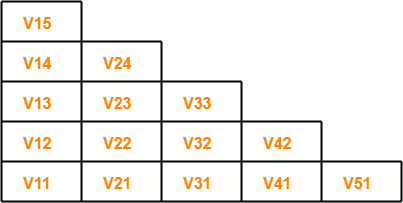
\includegraphics[width =8cm]{CYK-1.png}    
\end{center}

Let’s try to find the values of $V_{ij}$ for each cell. Where $V_{ij}$ represents a set of variables in the grammar which can derive the substring $x_{ij}$.\\
And there $x_{ij}$ represents the substring of a given word from index $i$ to index $j$.\\

\textbf{\textit{For Row1:}}\newline
\textit{For $V_{11}$:}\newline
$V_{11}$ represents the set of variables deriving $x_{11}$.\newline
$x_{11} = b$.
Only variable $B$ derives string b in the given grammar.\newline
Thus $V_{11}$ = \{$B$\}\newline

\textit{For $V_{21}$:}\\
$V_{21}$ represents the set of variables deriving $x_{21}$.\newline
$x_{21} = a$\newline
From given grammar variables $A$ and $C$ derive the character a.
Thus $V_{21}$ = $\{A, V\}$\\

\textit{For $V_{31}$:}\\
$V_{31}$ represents the set of variables deriving $x_{31}$.\newline
$x_{31} = a$\newline
From given grammar variables $A$ and $C$ derive the character a.
Thus $V_{21}$ = $\{A, C\}$\\

\textit{For $V_{41}$:}\\
$V_{31}$ represents the set of variables deriving $x_{41}$.\newline
$x_{41}$ = b.\newline
$x_{41}$ is equal  to $x_{11}$ so $V_{41}$ = $\{B\}$\\

\textit{For $V_{51}$:}\\
$V_{51}$ represents the set of variables deriving $x_{51}$.\newline
$x_{51}$ = b.
$x_{51}$ is equal to $x_{41}$ or $x_{31}$ so $V_{51}$ = $\{A, C\}$\\

For finding any row we have to take two paths first one is vertically up and other are diagonally. Then each column value of this row can be calculated by taking union of all multiplication of vertical and diagonal entry.\\
Like for row 2,\newline
$V_{ij}$ = $V_{ik}$ $V_{(i+k)(j-k)}$ where $k$ varies from 1 to $j-1$\newline
 
\textit{General formula:-}\\
\begin{center}
$\mathbf{V_{ij} = Union(V_{ik} V_{(i+k)(j-k)} )}$ where $k$ varies from 1 to $j-1$
\end{center}

\textbf{\textit{For Row 2:-}}\\
\textit{For $V_{12}$:-}\newline
There $i = 1$ and  $j = 2$ and $k = 1$\newline
Using general formula:-
\begin{align*}
V_{12} &= V_{11} \cdot V_{21}\\
V_{12} &= \{ B \} \{ A , C \}\\
V_{12} &= \{ BA \} \{ BC \}\\
\therefore V_{12} &= \{ A , S \}\\
\end{align*}

\textit{For $V_{22}$:-}\newline
There $i = 2$ and  $j = 2$ and $k = 1$
\begin{align*}
V_{22} &= V_{21} \cdot V_{31}\\
V_{22} &= \{ A, C \} \{ A , C \}\\
V_{22} &= \{ AA, AC, CA, CC \}\\
\end{align*}
Since $AA$, $AC$ and $CA$ do not exist, so we have-
\begin{align*}
V_{22} &= \{ CC \}\\
\therefore V_{22} &= \{ B \}\\
\end{align*}

\textit{For $V_{32}$:-}\newline
There $i = 3$ and  $j = 2$ and $k = 1$\newline
Substituting values in the formula, we get-
\begin{align*}
V_{32} &= V_{31} \cdot V_{41}\\
V_{32} &= \{ A, C \} \{ B \}\\
V_{32} &= \{ AB, CB \}\\
\end{align*}
Since $CB$ do not exist, so we have-
\begin{align*}
V_{32} &= \{ AB \}\\
\therefore V_{32} &= \{ S, C \}\\
\end{align*}

\textit{For $V_{42}$:-}\newline
There $i = 4$ and  $j = 2$ and $k = 1$\newline
Substituting values in the formula, we get-
\begin{align*}
V_{42} &= V_{41} \cdot V_{51}\\
V_{42} &= \{ B \} \{ A, C \}\\
V_{42} &= \{ BA, BC \}\\
\therefore V_{42} &= \{ A, S \}\\
\end{align*}

\textbf{\textit{For Row 3:-}}\\
\textit{For $V_{13}$:-}\newline
There $i = 1$ and  $j = 3$, $k = 1$ to (3-1) = 1, 2\newline
Substituting values in the formula, we get-
\begin{align*}
V_{13} &= V_{11} \cdot V_{22} \cup V_{12} V_{31}\\
V_{13} &= \{ B \} \{ B \} \cup \{ A , S \} \{ A , C \}\\
V_{13} &= \{BB\} \cup \{ AA, AC, SA, SC \}\\
\end{align*}
Since BB , AA , AC , SA and SC do not exist, so we have-
\begin{align*}
V_{13} &= \phi \cup \phi\\
\therefore V_{13} &= \phi\\
\end{align*}

\textit{For $V_{23}$:-}\newline
We have $i = 2$ , $j = 3$ , $k = 1$ to (3-1) = 1,2\newline
Substituting values in the formula, we get-
\begin{align*}
V_{23} &= V_{21} \cdot V_{32} \cup V_{22} V_{41}\\
V_{23} &= \{ A, C \} \{ S, C \} \cup \{ B \} \{ B \}\\
V_{23} &= \{AS, AC, CS, CC\} \cup \{ BB \}\\
\end{align*}
Since AS , AC , CS and BB do not exist, so we have-
\begin{align*}
V_{23} &= \{ CC \}\\
\therefore V_{23} &= B
\end{align*}

\textit{For $V_{33}$:-}\newline
We have $i = 3$ , $j = 3$, $k = 1$ to (3-1) = 1,2\newline
Substituting values in the formula, we get-
\begin{align*}
V_{33} &= V_{31} \cdot V_{42} \cup V_{32} V_{51}\\
V_{33} &= \{ A, C \} \{ A, S \} \cup \{ S, C \} \{ A, C \}\\
V_{33} &= \{AA, AS, CA, CS\} \cup \{ SA, SC, CA, CC \}\\
\end{align*}
Since AA , AS , CA , CS , SA , SC and CA do not exist, so we have-
\begin{align*}
V_{33} &= \phi \cup \{ CC \}\\
V_{33} &= \phi \cup \{ B\}\\
\therefore V_{33} &= B
\end{align*}

\textbf{\textit{For Row 4:-}}\\
\textit{For $V_{14}$:-}\newline
We have $i = 1$, $j = 4$, $k = 1$ to (4-1) = 1,2,3\newline
Substituting values in the formula, we get-
\begin{align*}
V_{14} &= V_{11} \cdot V_{23} \cup V_{12} V_{32} \cup V_{13} V_{41}\\
V_{14} &= \{ B \} \{ B \} \cup \{ A, S \} \{ S, C \} \cup \{ \phi, B \}\\
V_{14} &= \{ BB \} \cup \{AS, AC, SS, SC\} \cup \{ B \}\\
\end{align*}
Since BB , AS , AC , SS , SC and B do not exist, so we have-
\begin{align*}
V_{14} &= \phi \cup \phi \cup \phi\\
\therefore V_{14} &= \phi
\end{align*}

\textit{For $V_{24}$:-}\newline
We have $i = 2$ , $j = 4$ , $k = 1$ to (4-1) = 1,2,3\newline
Substituting values in the formula, we get-
\begin{align*}
V_{24} &= V_{21} \cdot V_{33} \cup V_{22} V_{42} \cup V_{23} V_{51}\\
V_{24} &= \{ A, C\} \{ B \} \cup \{ B \} \{ A, S \} \cup \{ B \} \{ A, C \}\\
V_{24} &= \{ AB, CB \} \cup \{BA, BS\} \cup \{ BA, BC \}\\
\end{align*}
Since CB does not exist, so we have-
\begin{align*}
V_{24} &= \{ AB \} \cup \{BA, BS\} \cup \{ BA, BC \}\\
V_{24} &= \{ S, C \} \cup \{A\} \cup \{ A, S \}\\
\therefore V_{24} &= \{ S, C, A \}
\end{align*}

\textbf{\textit{For Row 5:-}}\\
\textit{For $V_{15}$:-}\newline
We have $i = 1$ , $j = 5$ , $k = 1$ to (5-1) = 1, 2, 3, 4\newline
Substituting values in the formula, we get-
\begin{align*}\
V_{15} &= V_{11} V_{24} \cup V_{12} V_{33} \cup V_{13} V_{42} \cup V_{14} V_{51}\\
V_{15} &= \{ B\} \{ S, C, A \} \cup \{ A, S \} \{ B \} \cup \{ \phi \} \{ A, S \} \cup \{ \phi \} \{ A, C \}\\
V_{15} &= \{ BS, BC, BA \} \cup \{AB, SB\} \cup \{ A, S \} \cup \{A, C\}\\
\end{align*}
Since BS , SB , A , S and C do not exist, so we have-
\begin{align*}
V_{15} &= \{BC, BA\} \cup \{ AB \} \cup \phi \cup \phi\\
V_{15} &= \{S, A\} \cup \{ S, C \} \cup \phi \cup \phi\\
\therefore V_{15} &= \{ S, A, C \}
\end{align*}

After computing all $V_{ij}$ values for each cell, our triangular matrix looks like:-\\

\begin{center}
    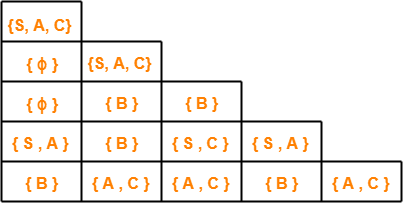
\includegraphics[width =10cm]{CYK-2.png}    
\end{center}

We can see that the value of $V_{15}$ contains the start symbol 'S'. Thus , string $x_{15}$ = ''baaba'' is a member of the language of given grammar.\newline

For calculating this matrix we can code it. Let's try to find an approach:-\\
We can see that for storing $V_{ij}$ we need a 2 D array. And for calculating each index $(i, j)$ we need it's column and diagonal to be already calculated. So, we can see that this call is recursive and we can use dynamic programming to calculate it.\\

\underline{Let's try to implement it’s pseudo code:-}\\

let the input be a string $I$ consisting of $n$ characters: $a_1 ... a_n$.\\
let the grammar contain $r$ nonterminal symbols $R_1 ... R_r$, with start symbol $R_1$.\\
let $P[n, n, r]$ be an array of booleans. Initialize all elements of $P$ to false.\\

\begin{lstlisting}[mathescape]
for each s = 1 to n
    for each unit production $R_v$ --> as
        set P[1, s, v] = true

for each l = 2 to n -- Length of span
    for each s = 1 to n-l+1 -- Start of span
        for each p = 1 to l-1 -- Partition of span
            for each production $R_a$ --> $R_b$ $R_c$
                if P[p, s, b] and P[l-p, s+p, c] then set P[l, s, a] = true

if P[n,1,1] is true then
    I is member of language
else
    I is not member of language
\end{lstlisting}
\underline{Time complexity:-}\\

\underline{Writing the running time as sum of for loops:}\\
\begin{center}
\LARGE{$T = \sum\limits_{i = 2}^{\infty} \sum\limits_{j = 1}^{n-i+1} \sum\limits_{k = 1}^{i-1} 1 $}\\
\end{center}
By solving this equation we obtain the expression,
\begin{align*}
T &= (n^3-n)/6\\
O(T) &= O(n^3)\\
\end{align*}
\underline{Space complexity:-}     We declare a 2 D array which have size $n \times n$ where $n$ is length of word.\\
Space complexity would be $O(n^2)$.\\

\chapter{Tree Decomposition}

\textbf{\textit{What is tree decomposition-:}} Simple it is mapping of a graph into a tree that can be used to define the tree width of the graph and speed up solving certain computational problems on the graph.

This is also known as junction trees, clique trees, joint trees. \\
 
And tree decomposition plays an important role in \textbf{probabilistic inference, constraint satisfaction, query optimization and matrix decomposition.}\\

This concept was introduced by Rudolf Halin(1976). Later it was rediscovered by Neil Robertson and Paul Seymour in 1984.\\

The decomposed tree T has the following \textbf{properties}-:\\
\textbf{1$>$} : The union of all sets nodes xi equals V. it means every vertex in graph G is at least inside one tree node.\\*
\textbf{2$>$} :for every edge(u,v) in the graph G, there exists at least one tree node that contains u and v.\\*
\textbf{3$>$} :If node Xi and Xj both contain a vertex V,then all nodes Xk along the (unique) path between Xi and Xj contain v as well.\\*
\begin{center}
    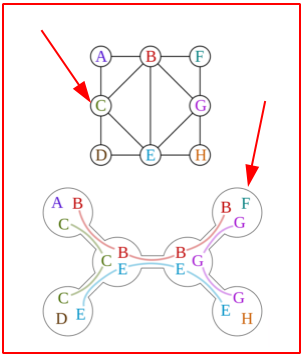
\includegraphics[width =8cm]{C5jV73V.png}    
\end{center}


From above definition , we can have two important \textbf{observations}-:\\
\newline
\textbf{1$>$} : From property 2, every edge has its two vertices both inside some tree nodes, but any two vertices u,v 
in a tree node doesn’t necessarily mean there is an edge
(U,,V).\\*
\textbf{2$>$} :From property 3, for any tree node X and its subtree Ti rooted in child Xi, Vi’ ={v belong to T-X} is independent with each other(no common vertices between Vi’) because if 2 nodes x1 and x2 have common vertex v , then v must be in X as well (ancestor X is along the unique path betweenX1 and X2). Therefore , if we exclude vertices in X from its subtree Ti, the remaining vertices Vi’ must be independent.\\*


*******(here Ti means T of i)*******

\chapter{Painting Fence Algorithm}
Given a fence with n posts and k colors, find out the number of ways of painting the fence such that at most 2 adjacent posts have the same color. Since the answer can be large, return it modulo $10^9 + 7$.\\*
Ex n=3 and k=2\\*
\newline
In this problem there are 6 possible ways of painting 3 posts with 2 colors.
\begin{center}
    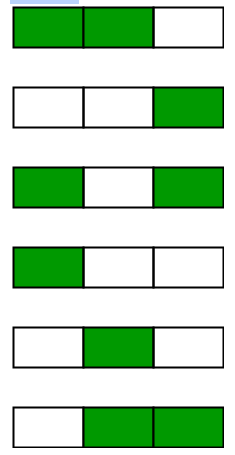
\includegraphics[width =5cm]{DhF7y5v.png}    
\end{center}
Consider the following image in which c, c’ and c” are respective colors of posts i, i-1 and i -2.\\*
\begin{center}
    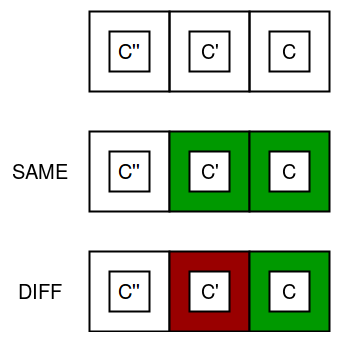
\includegraphics[width =5cm]{KDIJhWx.png}    
\end{center}
According to the constraint of the problem, c = c’ = c” is not possible simultaneously, so either c’ != c or c” != c or both. There are k – 1 possibilities for c’ != c and k – 1 for c” != c.\\*
\newline
\textbf{\textit{psuedo code:}}\\*
long countway(int n,int k)\\*
\{

\hspace{1cm}Long dp[n+1];\\ 
\hspace{1cm}long long mod=1000000007;\\ 
\hspace{1cm}memset(dp,0,n+1);\\*
\hspace{1cm}dp[1]=k,dp[2]=k*k;\\*
\hspace{1cm}for (int i = 3; i <= n; i++) \\*
\hspace{1cm}\{
    \newline
\hspace{1cm}\hspace{1cm}dp[i] = ((k - 1) * (dp[i - 1] + dp[i - 2])) % mod;
    \newline
\hspace{1cm}\}
    \newline
\hspace{1cm}return dp[n];
    \newline
\}
\newline
\textbf{\textit{Time complexity-:}}
O(n)\\*
\newline
\textbf{\textit{Space complexity-:}}
O(n)\\*

\chapter{Different ways to sum n using numbers greater than or equal to m
}
There are two natural are given n and m.The task is find the no. of ways in which the numbers that are greater than or equal to m can be added to get the sum n.\\
\newline
Let  n=x1+x2+x3+....+xr   given xi$>$=m where i={1,2,....,r}
and r can be 1 to n.
if m$>$n in this case there is no solution exist.\\
Example :  n=5,m=2\\
Total solutions=4 {(2+2+2),(3+3),(4+2),(6)}\\
We find solutions using dynamic programming. We declare 2-D matrix like dp[][].\\
\textbf{\textit{IF(i$<$j)}},dp[i][j]=0 because we can’t achieve sum i using the numbers which are greater than i.\\
\textbf{\textit{IF(i$=$j)}},dp[i][j]=1 sum=i=j,only one way to do this\\
\textbf{\textit{else}} dp[i][j]=dp[i][j+1] + dp[i-j][j] , sum i using numbers greater than or equal to j is equal to the sum of obtaining a sum of i using numbers greater than or equal to j+1 and obtaining the sum of i-j using numbers greater than or equal to j.\\

\textbf{pseudo code-:}\\
int numberofway(int n,int m)\\*
\{
\newline
\phantom{x} \hspace{3ex}int dp[n+2][n+2];\\*
\phantom{x} \hspace{3ex}memset(dp,0,sizeof(dp));\\*
\phantom{x} \hspace{3ex}dp[0][n+1]=1;\\*
\phantom{x} \hspace{3ex}for(int k=n;k$>$=m;k--)\\*
\phantom{x} \hspace{3ex}\{ \\*
\phantom{x} \hspace{3ex}\phantom{x} \hspace{3ex}for(int i=0;i$<$=n;i++)\\*\\*
\phantom{x} \hspace{3ex}\phantom{x} \hspace{3ex}\{ \\*
\phantom{x} \hspace{3ex}\phantom{x} \hspace{3ex}dp[i][k]=dp[i][k+1];\\*
\phantom{x} \hspace{3ex}\phantom{x} \hspace{3ex}if(i-k$>$=0)dp[i][k]+=dp[i-k][k]\\*
\phantom{x} \hspace{3ex}\phantom{x} \hspace{3ex}\} \\*
\phantom{x} \hspace{3ex}\} \\*
\phantom{x} \hspace{3ex}return dp[n][m];\\*

\} \\*
Time Complexity:
$O((n-m+1)(N)) ~ O(n^2)$ \\*
Space Complexity:
$O(n*m) ~ O(n^2)$ \\*
\newline
\newline

\textbf{\textit{K-th Largest Sum Contiguous Subarray:}} \\*
We have an array of integers. We find K-th largest sum of continuous subarray within the array of numbers which has negative and positive numbers.\\
\newline
Ex. a[]={20,-5,-1} and k=3 \\*
    subarray={20,15,14,-5,-6,-1} \\*
    3rd largest sum is 14   \\*
\textbf{Approach:} We create a sum array and store at ith place is a[0]+a[1]+...+a[i-1]. Given array is a[]. \\
Now for storing the Kth largest sum, use a min heap (priority queue) in which we push the contiguous sums till we get K elements, once we have our K elements, check if the element is greater than the Kth element it is inserted to the min heap with popping out the top element in the min-heap, else not inserted . At the end the top element in the min-heap will be your answer. \\


\textbf{\textit{Pseudo Code:}} \\*
int kthlagestsum(int arr[],int n,int k) \\*
\{ \\*
\phantom{x} \hspace{3ex}    int sum[n+1]; \\*
\phantom{x} \hspace{3ex}    sum[0]=0,sum[1]=arr[1];\\*
\phantom{x} \hspace{3ex}   for(int i=2;i<=n;i++) \\*
\phantom{x} \hspace{3ex}    sum[i]=sum[i-1]+arr[i-1];\\*
\phantom{x} \hspace{3ex}    priorityqueue<int, vector<int>, greater<int> > Q;\\*
\phantom{x} \hspace{3ex}    for(int i=1;i<=n;i++)\\*
\phantom{x} \hspace{3ex}    \{  \\*
\phantom{x} \hspace{3ex}\phantom{x} \hspace{3ex}        for(int j=i;j<=n;j++)  \\*
\phantom{x} \hspace{3ex}\phantom{x} \hspace{3ex}        \{ \\*
\phantom{x} \hspace{3ex}\phantom{x} \hspace{3ex}\phantom{x} \hspace{3ex}            int x=sum[j] - sum[i-1];\\*
\phantom{x} \hspace{3ex}\phantom{x} \hspace{3ex}\phantom{x} \hspace{3ex}            if(Q.size() < k)Q.push(x);\\*
\phantom{x} \hspace{3ex}\phantom{x} \hspace{3ex}\phantom{x} \hspace{3ex}            else\\*
\phantom{x} \hspace{3ex}\phantom{x} \hspace{3ex}\phantom{x} \hspace{3ex}            {\\*
\phantom{x} \hspace{3ex}\phantom{x} \hspace{3ex}\phantom{x} \hspace{3ex}\phantom{x} \hspace{3ex}                if(Q.top()<x)Q.pop(),Q.push(x);\\*
\phantom{x} \hspace{3ex}\phantom{x} \hspace{3ex}\phantom{x} \hspace{3ex}            }\\*
\phantom{x} \hspace{3ex}\phantom{x} \hspace{3ex}        \}\\*

    
\phantom{x} \hspace{3ex}    \}
\phantom{x} \hspace{3ex} return Q.top();   
\} \\*
\newline
Time Complexity:
$O(n^2 * log(k))$ \\*
Space Complexity:
$O(k)$ \\*

\textbf{\textit{Sequences of given length where every element is more than or equal to twice of previous:}}
Given two integers n and m. \\*
Find : Possibles sequences of length n such that each of the next element is greater than or equal to twice of previous element but less than m. \\
\newline
Example : n=4 and m=10 \\
\newline
Possible sequences=\{1,2,4,8\} ,\{1,2,5,10\},\{1,2,4,9\},\{1,2,4,10\} \\
\newline
So answer=4\\
\newline
There are 2 possibilities for n-th element \\*
\textbf{1$>$} : If it is m,then (n-1)th element is at most m/2. We recur for m/2 and n-1. \\*
\textbf{2$>$} :If it is not m, then it is at most is m-1. We recur for (m-1) and n.\\*
So the total no. of sequences is the sum of first (no. of sequences of length n and max value m-1) and second(no. Of sequences of length n-1 and max value m/2).\\
\newline
\newline
\textbf{\textit{Pseudo Code:}} \\*
int getTotalSeq(int m,int n)
\{ \\*
    if(m<n)return 0;\\*
    if(n==0)return 1;\\*
    return getTotalSeq(m-1,n) + getTotalSeq(m/2,n-1);\\*

\} \\*
\newline
\newline
\textbf{\textit{Pseudo Code using DP:}} \\*
int getTotalSeq(int m,int n)\\*
\{ \\*
\phantom{x} \hspace{3ex}    int dp[m+1][n+1];\\*
\phantom{x} \hspace{3ex}    for(int i=0;i<m+1;i++)\\*
\phantom{x} \hspace{3ex}    \{ \\*
\phantom{x} \hspace{3ex}\phantom{x} \hspace{3ex}        for(int j=0;j<n+1;j++)\\*
\phantom{x} \hspace{3ex}\phantom{x} \hspace{3ex}        \{ \\*
\phantom{x} \hspace{3ex}\phantom{x} \hspace{3ex} \phantom{x} \hspace{3ex}           if(i==0 || j==0)dp[i][j]=0\\*
\phantom{x} \hspace{3ex}\phantom{x} \hspace{3ex} \phantom{x} \hspace{3ex}           else if (i<j)dp[i][j]=0;\\*
\phantom{x} \hspace{3ex}\phantom{x} \hspace{3ex} \phantom{x} \hspace{3ex}           else if(j==1)dp[i][j]=i;\\*
\phantom{x} \hspace{3ex}\phantom{x} \hspace{3ex} \phantom{x} \hspace{3ex}          else dp[]i][j]=dp[i-1][j] + dp[i/2][j-1];\\*
\phantom{x} \hspace{3ex} \phantom{x} \hspace{3ex}       \} \\*
\phantom{x} \hspace{3ex}    \} \\*
\phantom{x} \hspace{3ex} return dp[m][n];

\} \\*
\newline
Time Complexity:
$O(m*n)$ \\*
Space Complexity:
$O(m*n)$ \\*
\newline

\chapter{K-th Largest Sum Contiguous Subarray}
We have an array of integers. We find $K^{th}$ largest sum of continuous subarray within the array of numbers which has negative and positive numbers.\newline\newline
Ex.\newline
a[ ] = $\mathtt{\{20, -5, -1\}}$ and $k = 3$\newline
	subarray = $\mathtt{\{20, 15, 14, -5, -6, -1\}}$\newline
	\textbf{3$^{rd}$ largest sum is 14}\newline\newline

\underline{Approach:} We create a sum array and store at $i^{th}$ place is $a[0] + a[1] + ... + a[i-1]$.
\newline
Given array is $a$[ ].\newline
Now for storing the $K^{th}$ largest sum, use a min heap (priority queue) in which we push the contiguous sums till we get $K$ elements, once we have our $K$ elements, check if the element is greater than the $K^{th}$ element it is inserted to the min heap with popping out the top element in the min-heap, else not inserted . At the end the top element in the min-heap will be your answer.\newline\newline

\underline{Pseudo Code:}\newline
\begin{lstlisting}
int kthlagestsum(int arr[],int n,int k)
{
	int sum[n+1];
	sum[0]=0,sum[1]=arr[1];
	for(int i=2;i<=n;i++)sum[i]=sum[i-1]+arr[i-1];

	priority_queue<int, vector<int>, greater<int> > Q;

	for(int i=1;i<=n;i++)
	{
		for(int j=i;j<=n;j++)
		{
			int x=sum[j] - sum[i-1];
			if(Q.size() < k)Q.push(x);
			else
			{
				if(Q.top()<x)Q.pop(),Q.push(x);
			}
		}
	}
	return Q.top();
}
\end{lstlisting}

\underline{Time Complexity:}   $O(n^2 \times log(k))$\newline\newline
\underline{Space Complexity:}  $O(k)$\newline

\chapter{Sequences of given length where every element $\mathbf{\geq}$ twice of previous}
Given two integers $n$ and $m$.\newline
Find : Possibles sequences of length $n$ such that each of the next element is $\geq$ twice of previous element but $<$ m.\newline\newline
Example : $n = 4$ and $m = 10$\newline
Possible sequences = $\mathtt{\{1,2,4,8\}, \{1,2,5,10\}, \{1,2,4,9\}, \{1,2,4,10\}}$\newline
So answer = 4\newline\newline
There are 2 possibilities for $n^{th}$ element\newline
If it is $m$, then $n-1^{th}$ element is at most $m/2$. We recur for $m/2$ and $n-1$.\newline
If it is not $m$, then it is at most is $m-1$. We recur for $m-1$ and $n$.\newline
So the total no. of sequences is the sum of first (no. of sequences of length $n$ and max value $m-1$) and second (no. of sequences of length $n-1$ and max value $m/2$).\newline

\underline{Pseudo Code:}\newline
\begin{lstlisting}
int getTotalSeq(int m,int n)
{
	if(m<n)return 0;
	if(n==0)return 1;
	return getTotalSeq(m-1,n) + getTotalSeq(m/2,n-1);
}

Pseudo Code using DP:
int getTotalSeq(int m,int n)
{
	int dp[m+1][n+1];
	for(int i=0;i<m+1;i++)
	{
		for(int j=0;j<n+1;j++)
		{
			if(i==0 || j==0)dp[i][j]=0
			else if (i<j)dp[i][j]=0;
			else if(j==1)dp[i][j]=i;
			Else dp[]i][j]=dp[i-1][j] + dp[i/2][j-1];
	}
	return dp[m][n];
}
\end{lstlisting}
\underline{Time Complexity:}  $O(m \cdot n)$\newline\newline
\underline{Space Complexity:} $O(m \cdot n)$\newline\newline

\chapter{Convert to Strictly increasing integer array with minimum changes}
Given: An array with n integers.\\
\newline
Find : Get Strictly increasing array by minimum change in original array.\\
\newline
Ex. arr[]=\{1,2,6,5,4\} \\
\newline
Output array={1,2,4,5,6} by only 2 changes. \\
\newline
LIS-longest increasing subsequence. We have to change those elements which are not part of LIS. So the minimum element to change is different of size of array and the number are integers. So while making LIS, we so not consider those element as part of LIS that cannot from strictly increasing by inserting elements in middle.\\
\newline
\textbf{\textit{Pseudo Code:}} \\*
int minRemove(int arr[],int n)
\{ \\*
\phantom{x} \hspace{3ex}    int LIS[n],l=0; \\*
\phantom{x} \hspace{3ex}    for(int i=0;i<n;i++)LIS[i]=1;\\*
    
\phantom{x} \hspace{3ex}    for(int i=1;i<n;i++)\\*
\phantom{x} \hspace{3ex}    \{ \\*
\phantom{x} \hspace{3ex} \phantom{x} \hspace{3ex}       for(int j=0;j<i;j++)\\*
\phantom{x} \hspace{3ex} \phantom{x} \hspace{3ex}       \{ \\*
\phantom{x} \hspace{3ex} \phantom{x} \hspace{3ex} \phantom{x} \hspace{3ex}          if(arr[i] $>$ arr[j] and (i-j)$<$=(arr[i]-arr[j])) LIS[i]=max(LIS[i],LIS[j] +1);\\*
\phantom{x} \hspace{3ex} \phantom{x} \hspace{3ex}       \} \\*
\phantom{x} \hspace{3ex}\phantom{x} \hspace{3ex}len=max(len,LIS[i]);

\phantom{x} \hspace{3ex}    \} \\*
\phantom{x} \hspace{3ex}return n-len; \\*
\} \\*
\newline
Time Complexity:
$O(n^2)$ \\*
Space Complexity:
$O(n)$ \\*
\newline
\newline
\chapter{Min cost path}
Statement-: you have given a cost matrix where each block represents it’s cost. You have to go from (0,0) to (m,n) with minimum total cost where
Total cost is the sum of all block costs where you visited.or you can only traverse down, right,and diagonally lower cells from a given cell. Means from (i,j) you can go (i,j+1) or (i+1,j) or (i+1,j+1). Remember that all costs are positive. \\*
\newline

For a given example what is the minimum cost path to(2,2)? \\*
\begin{center}
    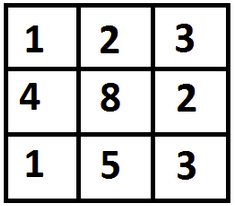
\includegraphics[width =5cm]{90JsYvl.png}    
\end{center}
Obviously it is the path which follows the following path. \\*
(0,0)-$>$(0,1)-$>$(1,2)-$>$(2,2). The total cost of this path is  \\*
cost=8 because we visited the cell with cost 1,2,2,3 and their sum is equal to 8. \\*
\begin{center}
    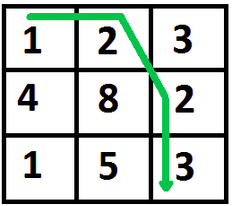
\includegraphics[width =5cm]{UYv9kel.png}    
\end{center}
You can see that it simply follow recursion. \\*
Let’s think about it. \\*
Let’s assume that finally we are at (m,n) then we can say that either we come from (m-1,n) or (m,n-1) or (m-1,n-1). \\*
So we got that \\*
mincost(m,n)=minimum(mincost(m-1,n),mincost(m,n-1),mincost(m-1,n-1)) \\*
From this equation we can say that it simply follow recursion. \\*
\textbf{\textit{Pseudo code-:}} \\*
Declare function(int mincost(int m,int n) \\*
Base conditions are followings-:\\*
if(n$<$0) \\*
\phantom{x} \hspace{3ex}Return infinity;\\*
if(m$<$0)\\*
\phantom{x} \hspace{3ex}Return infinity;\\*
If (m==0 and n==0)\\*
\phantom{x} \hspace{3ex}Return cost[m][n];\\*
Return cost[m][n]+minimum(mincost(m-1,n),mincost(m,n-1),mincost(m-1,n-1));\\*
\newline
\newline
\newline
Complexity analysis-: \\*
\phantom{x} \hspace{3ex} Time complexity-:\\
For every step calculation we make 3 stacks until they are not zero so time complexity would be $3^{maximum(m,n)}$; \\*
Space complexity-: \\*
We only filling cost[m][n] for whole process so space complexity would be O(m*n);
Now you can see that we are calculating subproblem over and over so why we can’t use dynamic programming.
Definitely we can use it \\*
Let’s assume ‘mn(i,j)' refers the minimum cost  to reach (i,j) from (0,0); \\*
Then for  mn(2,2) we need to calculate mn(1,1) and mn(1,2) and mn(2,1).\\*
And for mn(1,1) we need  to calculate mn(0,0) and mn(1,0) and mn(0,1).\\*
Then for  mn(1,2) we need to calculate mn(0,1) and mn(0,2) and mn(1,1).\\*
Then for  mn(2,1) we need to calculate mn(1,1) and mn(2,0) and mn(1,0).\\*
\newline
From this you can see that we need to calculate mn(1,1) twice and many others. So if we calculate it once and then store it in an array then we not need to calculate it again.\\*
int minCost(int cost[R][C], int m, int n)
\{ \\*
\phantom{x} \hspace{3ex}     int i, j;\\*
  
\phantom{x} \hspace{3ex}     // Instead of following line, we can use int tc[m+1][n+1] or \\*
\phantom{x} \hspace{3ex}     // dynamically allocate memory to save space. The following line is\\*
\phantom{x} \hspace{3ex}     // used to keep the program simple and make it working on all compilers.\\*
\phantom{x} \hspace{3ex}     int tc[R][C];  \\*
\phantom{x} \hspace{3ex}     tc[0][0] = cost[0][0];\\*
  
\phantom{x} \hspace{3ex}     /* Initialize first column of total cost(tc) array */\\*
\phantom{x} \hspace{3ex}     for (i = 1; i <= m; i++)\\*
\phantom{x} \hspace{3ex} \phantom{x} \hspace{3ex}       tc[i][0] = tc[i-1][0] + cost[i][0];\\*
  
\phantom{x} \hspace{3ex}     /* Initialize first row of tc array */\\*
\phantom{x} \hspace{3ex}     for (j = 1; j <= n; j++)\\*
\phantom{x} \hspace{3ex} \phantom{x} \hspace{3ex}       tc[0][j] = tc[0][j-1] + cost[0][j];\\*
  
\phantom{x} \hspace{3ex}     /* Construct rest of the tc array */\\*
\phantom{x} \hspace{3ex}     for (i = 1; i <= m; i++)\\*
\phantom{x} \hspace{3ex}  \phantom{x} \hspace{3ex}      for (j = 1; j <= n; j++)\\*
\phantom{x} \hspace{3ex}  \phantom{x} \hspace{3ex} \phantom{x} \hspace{3ex}         tc[i][j] = min(tc[i-1][j-1], 
                           tc[i-1][j], 
                           tc[i][j-1]) + cost[i][j];
  
\phantom{x} \hspace{3ex}     return tc[m][n]; \\*


\} \\*
\newline
\newline
Time complexity-:\\
There are 3 loops and one of them is a nested loop so total time complexity would be some of all of this.
T=sum(‘sigma(i=1,m)1+’sigma’(i=1,n)1+’sigma’(i,m)’sigma’(j,n)1) \\
T=m+n+m*n \\*
Time complexity O(m+n+m*n); \\*\\*
Space complexity-: there space complexity are 2*m*n one of m*n is for storing cost and other m*n are calculating mincost(i,j).\\*
Space complexity=O(2*m*n)\\*

\chapter{Newman-Conway sequence}
newman -conway sequence is 1,1,2,2,3,4,4,4,5,6,7,7…. \\*
In mathematics term newman-conway numbers is defined by recurrence relation \\*
f(n)=f(f(n-1))+f(n-f(n-1))\\*
Where base condition are that\\* 
f(1)=1 and f(2)=1.\\*
You can solve this problem using recursion.like you solve fibonacci. \\*
\newline
\newline
\textbf{\textit{Pseudo Code:}} \\*
Int seq(int n) \\*
{ \\*
Base conditions-:\\*
if(n==1)\\*
\phantom{x} \hspace{3ex}Return 1;\\*
if(n==2)\\*
\phantom{x} \hspace{3ex}Return 1;\\*
Return seq(seq(n-1))+seq(n-seq(n-1));\\*
}
But recursion solutions have $2^n$ complexity because n to 1 there will be 2 partition of every part.means
For f(4)=f(3)+f(4-f(3) there you have to call f(3) two time \\
\newline
And for f(3)=f(2)+f(3-f(2)) there also you have to call f(2) two times so totally you have to call $2^n$ for calculating nth number of newman-convey sequence.\\
\newline
We had been seen that this is recalculating the values
So there we can use dynamic programming.\\
\newline
Declare a array whose ith index store ith number of newman-convey sequence.\\
\newline
Int f[n+1]; \\*
Base condition f[1]=1 and f[2]=1;\\*
for(int i=3;i<=n;i++)\\*
f[i]=f[i-1]+f[i-f[i-1]];\\*


Time complexity-:\\*
There is only one for loop so \\*
T=sigma(i=3,n+1)1;\\*
T=n-2; \\*
So time complexity O(n)\\*
\newline
\newline
Space complexity-:\\*
There is f[n] array and we are filling it to pre-calculate all newman-conway sequence.\\*
So space complexity is O(n). \\*

\chapter{ Shortest Common Subsequence}
In this problem you are given two strings and we have to find the length of the shortest string that has both the given strings as subsequences.\\
\newline
We will solve this by using bottom up DP. We will process the strings character by character and store the results for every pair of prefixes of string1 and string2.\\
\newline Let’s understand this with an example, given two strings\\*
String 1 - APQRSTU \\*
String 2 - KPLRMNTUO \\*
Then the length of shortest string that has both the given strings  - 12 is AKPQLRSMNTUO\\*
$\#$include$<$iostream$>$ \\*
$\#$include$<$string$>$\\*

using namespace std;\\*

int shortestcommonsubseq(string str1, string str2)\\*
\{ \\*
\phantom{x} \hspace{3ex}    int l1 = str1.length(), l2 = str2.length();\\*
\phantom{x} \hspace{3ex}    int dp[l1 + 1][l2 + 1];\\*
    
\phantom{x} \hspace{3ex}    //intialisation\\*
\phantom{x} \hspace{3ex}    for(int i = 0; i $<$= l1; i++)\\*
\phantom{x} \hspace{3ex} \phantom{x} \hspace{3ex}       dp[i][0] = i;\\*
\phantom{x} \hspace{3ex}    for(int j = 0; j $<$= l2; j++)\\*
\phantom{x} \hspace{3ex} \phantom{x} \hspace{3ex}       dp[0][j] =j;\\*
\phantom{x} \hspace{3ex}    for(int i = 1; j $<$= l1; i++)\\*
\phantom{x} \hspace{3ex} \phantom{x} \hspace{3ex}       for(int j = 1; j $<$= l2; j++)   \\* 
\phantom{x} \hspace{3ex} \phantom{x} \hspace{3ex}  \phantom{x} \hspace{3ex}         if(str1[i-1] == str2[j-1])\\*
\phantom{x} \hspace{3ex}  \phantom{x} \hspace{3ex} \phantom{x} \hspace{3ex} \phantom{x} \hspace{3ex}           dp[i][j] = dp[i-1][j-1] + 1;\\*
\phantom{x} \hspace{3ex} \phantom{x} \hspace{3ex}  \phantom{x} \hspace{3ex}         else\\*
\phantom{x} \hspace{3ex} \phantom{x} \hspace{3ex} \phantom{x} \hspace{3ex}  \phantom{x} \hspace{3ex}            dp[i][j] = min(dp[i - 1][j], dp[i][j - 1]) + 1;\\*

\} \\*
int main()\\*
\{\\*
\phantom{x} \hspace{3ex}    string str1, str2;\\*
\phantom{x} \hspace{3ex}    cout $<<$ “Enter string 1 ”;\\*
\phantom{x} \hspace{3ex}    getline(cin,str1);\\*
\phantom{x} \hspace{3ex}    cout $<<$ “Enter string 2” ;\\*
\phantom{x} \hspace{3ex} \phantom{x} \hspace{3ex}       getline(cin,str2);\\*
\phantom{x} \hspace{3ex}    cout $<<$ “Length of the shortest common subsequence is ” $<<$ endl;\\*
\phantom{x} \hspace{3ex}    cout $<<$ shortestcommonsubseq(str1, str2) $<<$ endl;\\*
\phantom{x} \hspace{3ex}    return 0;\\*
\}\\*

\chapter{Gold mine problem}
In this problem we are given gold mine of  n*m dimension. Each field contain a positive integer which is the amount of gold in tons. Initially the miner is at first column  but can be at any row. He can move only in two ways \\
\textbf{1$>$} : Diagonally up toward the right (/). \\*
\textbf{2$>$} : Right (-$>$).\\*\\*
\textbf{3$>$} : Diagonally down toward the right ( ).\\*\\*
We have to find the maximum amount of gold? \\*
Ex. given mat[][]=\{\{1 ,3 , 1 ,5\},\\*
             \{2 ,2 ,4 ,1 \},\\*
             \{5 , 0, 2, 3\},\\*
             \{0 ,6 ,1 ,2\}\}\\*
Output : 16  \\*
        way: \{(2,0)-$>$(1,1)-$>$(1,2)-$>$(0,3)\}\\*
            Or \{(2,0)-$>$(3,1)-$>$(2,2)-$>$(2,3)\}\\*

\textbf{\textit{Psuedo Code:}}\\*
int getmaxgold(int gold[][],int m,int n)
\{ \\*
\phantom{x} \hspace{3ex}    int goldTable[m][n];\\*
\phantom{x} \hspace{3ex}    memset(goldTable,0,sizeof(goldTable));\\*
    
\phantom{x} \hspace{3ex}    for(int col=n-1;col$>$=0;col--)\\*
\phantom{x} \hspace{3ex} \phantom{x} \hspace{3ex}       for(int row=0;row$<$m;row++)\\*
\phantom{x} \hspace{3ex} \phantom{x} \hspace{3ex}       \{ \\*
\phantom{x} \hspace{3ex} \phantom{x} \hspace{3ex} \phantom{x} \hspace{3ex}          int right=(col==n-1)? 0 : goldTable[row][col+1];\\*
\phantom{x} \hspace{3ex} \phantom{x} \hspace{3ex} \phantom{x} \hspace{3ex}          int rightup=(row==0 || col==n-1) ? 0 : goldTable[row-1][col+1];\\*
\phantom{x} \hspace{3ex} \phantom{x} \hspace{3ex} \phantom{x} \hspace{3ex}          int rightdown=(row==m-1 || col==n-1)? 0: goldTable[row+1][col+1];\\*

\phantom{x} \hspace{3ex} \phantom{x} \hspace{3ex} \phantom{x} \hspace{3ex}          mx=max(right,max(rightup,rightdown));\\*
\phantom{x} \hspace{3ex} \phantom{x} \hspace{3ex} \phantom{x} \hspace{3ex}          goldTable[row][col]=gold[row][col] + mx;\\*

\phantom{x} \hspace{3ex} \phantom{x} \hspace{3ex}       \} \\*
\phantom{x} \hspace{3ex}        int res=goldTable[0][0];\\*
\phantom{x} \hspace{3ex}        for(int i=1;i$<$m;i++)res=max(res,goldTable[i][0]);\\*
\phantom{x} \hspace{3ex}  return res;

\} \\* 

First create 2-D matrix goldTble[m][n]. Amount of gold is always positive. So we would like to cover maximum values under given constraints.In every move , we move one step toward right side. So we always end up in last column. If we are at the last column, then we can’t move right.\\
\newline
If we are at the first row or last column, then we just assign 0 otherwise assign the value of goldTable[row-1][col+1] to rightup. \\
\newline
If we are at the last row or last column, then we just assign 0 otherwise assign the value of goldTable[row+1][col+1] to rightup. \\
\newline
Now we find max of right,rightup,rightdown and then add it with that mat[row][col].
Lastly find the max of all rows and first column and return it. \\
\newline
\newline
Time Complexity:
$O(n*m)$ \\*
Space Complexity:
$O(m*n)$ \\*
\newline
\newline
\chapter{Greedy and dynamic programming}
A greedy algorithm is an algorithmic paradigm that builds up a solution piece by piece, always choosing the next piece that offers the most obvious and immediate benefit. So the problems where choosing locally optimal also leads to a global solution are best fit for Greedy. \\
\newline

For example take the problem ‘ fractional knapsack problem'. the local optimal strategy is to choose the item that has maximum value vs  weight ratio. This strategy also leads to a global optimal solution because we allowed taking fractions of an item.\\
\newline

Finally, the conclusion is that for greedy algorithms , we make whatever choice seems best at the moment in the hope that it will lead to a global optimal solution. In dynamic programming we make decisions at each step considering current problem and  solution to previously solved sub-problem to calculate optimal solution.\\
\newline

Major differences between greedy method and dynamic programming-: \\*

Feasibility-:  \\*
In greedy-: \\*
                    We make best at a time who leads for the final optimal solution.
In dynamic programming-: in this we make a decision who takes the best solution from all subproblem we solved now.\\*

Optimal-:\\*
In greedy-:\\*
In greedy methods sometimes there is no guarantee that we get the optimal solution.but in most in cases it is possible.\\*
In dynamic programming-:\\*
We can be sure that we can get the optimal solution because we take the best solution among all subproblems.or we can say that in general it will generate an optimal solution using principle of optimality.\\*

recursion-:\\*
In greedy-:\\*
                   In this we make locally optimal choices at each stage.

In dynamic programming-: Dynamic programming is an algorithmic technique which is usually based on a recurrent formula that uses some previously calculated states.\\*

Memorization-: \\*
In greedy-: \\*
It is more efficient than dynamic solution because we never  look at back or revise previous choices
For dynamic programming we already discussed it. \\*

Time complexity-: \\*
Greedy approaches are generally faster than dynamic programming. Reason it same that we take for memorization.\\*
Space complexity-: \\*
Most of the cases both the approaches have the same space complexity.\\*

Working method-:\\*
In greedy-: \\*
          The greedy method computes its solution by making its choices in a serial forward fashion, never looking back or revising previous choices.\\*

In dynamic programming-:Dynamic programming computes its solution bottom up or top down by synthesizing them from smaller optimal sub solutions.\\*

Examples-: \\* 
Greedy-:\\*
Dijkstra’s shortest path algorithm, fractional knapsack.\\*

Dynamic programming-:\\*
Bellman ford algorithm , 0/1 knapsack problem.\\*

Let’s understand all qualities taking by example\\*

Dijkstra’s vs bellman ford-:\\*
We are comparing these both algorithms because they both are used for the shortest path from a given node to all other nodes in a given graph.\\*

 Brief introduction to dijkstra algorithm-: at every step we take node a node and update the distance of all connected vertices and update their distance. For do this we use priority queue which give us a node having minimum distance from source .\\*

We already discussed bellman ford where you can see that it is used for negative edges. \\*

In the Dijkstra algorithm we can see that at every step we pick all connected edges of a given node and update the distance of the node. We can’t take care of what happened in previous and be sure about what is best decision in current condition\\*

For  these both algorithms the space complexity is the same; it is O(v).
But the time complexity would not be the same. Dijkstra has far better complexity than Bellman ford.\\*
\newline
It is (Elog(v)+vlog(v)) where E is number of edges in a given graph.
But we can see that bellman have O(vE) which are more greater than dijkstra’s algorithm. \\*


\chapter{0 - 1 Knapsack Problem}
\textbf{\textit{Firstly let’s know what the problem really is?}} \\*
\newline
Problem Statement - There is a thief who is robbing a store and can carry a maximal weight of W into his knapsack. There are n items in total and weight of ith item is wi and the profit of selecting this item is pi. So the question is , in what way he should select the items so that he could earn  maximum profit.\\*
\newline
In 0-1 knapsack , items can not be broken which means the thief should take the item as a whole or should leave it. This is the reason behind calling it as 0-1 knapsack.\\*
\newline
First we solve it using recursion. For this the method is too simple.\\*
\newline
We have to make all subsets and then calculate their total weights and the we have to consider those such that the total weight is smaller than W. And then from all those subsets we will choose the maximum.\\*
\newline
So there can be two cases only\\*
\textbf{1$>$} : The item is included in the optimal structure.\\*
\textbf{2$>$} : The item is not included in the optimal structure.\\*
\newline
Thus, the maximum value that can be obtained from ‘n’ items is the max of the following two values.\\*
\textbf{1$>$} : Maximum value obtained by n -1 items and W weight(excluding nth item).\\*
\textbf{2$>$} : Value of nth item plus maximum value obtained by n-1 items and W minus the weight of the nth term(including nth item).\\*
\newline
If the weight of ‘nth’ item is greater than ‘W’, then the nth item cannot be included and Case 1 is the only possibility.\\*

Below is the using recursion.\\*
\newline
$\#$include $<$bits/stdc++.h$>$ \\*
using namespace std; \\*
int max(int a, int b) { return (a $>$ b) ? a : b; } \\*

int knapSack(int W, int wt[], int val[], int n) \\*
\{ \\*
\phantom{x} \hspace{3ex}    if (n == 0 || W == 0) \\*
\phantom{x} \hspace{3ex} \phantom{x} \hspace{3ex}       return 0; \\*
\phantom{x} \hspace{3ex}    if (wt[n - 1] $>$ W) \\*
\phantom{x} \hspace{3ex} \phantom{x} \hspace{3ex}       return knapSack(W, wt, val, n - 1); \\*
\phantom{x} \hspace{3ex}    else\\*
\phantom{x} \hspace{3ex} \phantom{x} \hspace{3ex}       return max( 
            val[n - 1] 
                + knapSack(W - wt[n - 1], \\*
                        wt, val, n - 1), \\*
\phantom{x} \hspace{3ex}\phantom{x} \hspace{3ex}    knapSack(W, wt, val, n - 1)); \\*

\}\\*
\newline
int main() 
\{ \\* 
\phantom{x} \hspace{3ex}    int val[] = { 60, 100, 120 }; \\*
 \phantom{x} \hspace{3ex}   int wt[] = { 10, 20, 30 }; \\*
\phantom{x} \hspace{3ex}    int W = 50; \\*
\phantom{x} \hspace{3ex}    int n = sizeof(val) / sizeof(val[0]); \\*
\phantom{x} \hspace{3ex}    cout $<<$ knapSack(W, wt, val, n); \\*
\phantom{x} \hspace{3ex}    return 0; \\*
\} \\* 
\newline
\newline
It can’t be solved by Greedy approach. Greedy approach does not ensure an optimal solution. In many instances, Greedy approach may give an optimal solution. For example in case of fractional knapsack.\\
\newline

Let’s see what a fractional knapsack.\\
In this case items can be broken into smaller pieces , hence the thief can select fractions of items. That is, the thief may take only a fraction $x^i$ of $i^{th}$ item. 
0 $\leq= x_i$ $<$= 1.\\
\newline
If we first sort pi/wi in decreasing order, it is clear that an optimal solution must fill the knapsack exactly, otherwise we could add a fraction of one of the remaining items and increase the overall profit.\\
\newline
Thus , an optimal solution can be obtained by\\
    sigma(xi * wi) = W
    
Since we can’t use fractional objects here we can’t use greedy algorithms in the 0-1 knapsack problem.\\
\newline
Let’s understand this with an example :-\\*
Let’s consider 3 items A, B and C. There Price and weight is given as follows :-\\*

\begin{center}
    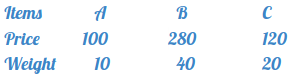
\includegraphics[width =8cm]{71GurBu.png}    
\end{center}
Now let’s consider the capacity of the knapsack to be W = 60.\\*
\newline
Now if we use the greedy approach, first item A is selected. Then, the next B is chosen . Hence , total profit is 100 + 280 = 380. However, the optimal solution of this instance can be achieved by selecting items, B and C, where the total profit is 280 + 120 = 400.\\*
Hence it is proved that a greedy approach will not work here. We will solve it using DP.\\*
\newline
In the DP approach we will be considering the same cases as we mentioned in the recursive approach. Firstly we will create a table DP[][] in which in the column we will write from 0 to the capacity of the knapsack and in the row we will consider all possible weights including 0. So the first column and row which states either 0 capacity or 0 weight is filled initially with 0. The cell DP[i][j] will denote the maximum value at ‘j-weight’ considering all the values from ‘1 to ith’. So if we consider ‘wi’(weight in ‘ith’ row) we can fill it in all columns which have ‘weight values > wi’. So here we have only two options :\\*
\textbf{1$>$} :Fill ‘wi’ in the column.\\*
\textbf{2$>$} : Do not fill ‘wi’ in the given column.\\*

Now we have to take a maximum of these two possibilities, formally if we do not fill ‘ith’ weight in ‘jth’ column then DP[i][j] state will be same as DP[i-1][j] but if we fill the weight, DP[i][j] will be equal to the value of ‘wi’+ value of the column weighing ‘j-wi’ in the previous row. So we take the maximum of these two possibilities to fill the current state. \\
\newline
Now understand this with an example.\\*
Let the weight elements = \{1,2,3\}\\*
Let wight values = \{10,15,40\}\\*
Capacity = 6.\\*
\begin{center}
    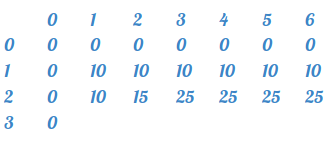
\includegraphics[width = 8cm]{nbGvAsc.png}    
\end{center}
Explaination:\\*
So when we are filling ‘weight = 2’ we come across ‘j = 3’ and there we take maximum of (10, 15 + DP[1][3 -2]).\\*
\newline
And since we know the value the value of DP[1][1] = 10. \\*
Thus max(10, 15 + Dp[1][1]) = 25.\\*
Using this similarly we conclude the following table.\\*
\begin{center}
    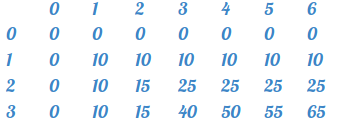
\includegraphics[width = 8cm]{ilDYzPq.png}    
\end{center}
Thus the maximum profit we can earn is 65.\\*
\newline
Time Complexity:
$O(N*W)$ \\*
Auxiliary Complexity:
$O(N*W)$ \\*
The use of 2-D array of size ‘N*W’.\\*

Below is the code for 0-1 knapsack using DP. \\*
$\#$include $<$stdio.h$>$ \\*
int max(int a, int b) \\*
\{ \\*
\phantom{x} \hspace{3ex}    return (a $>$ b) ? a : b; \\*
\} \\*
\newline
int knapSack(int W, int wt[], int val[], int n) \\*
\{ \\*
\phantom{x} \hspace{3ex}\phantom{x} \hspace{3ex}    int i, w; \\*
\phantom{x} \hspace{3ex}\phantom{x} \hspace{3ex}    int K[n + 1][W + 1]; \\*
\phantom{x} \hspace{3ex}\phantom{x} \hspace{3ex}    for (i = 0; i $>$= n; i++) \\*
\phantom{x} \hspace{3ex}\phantom{x} \hspace{3ex}    \{ \\*
\phantom{x} \hspace{3ex}\phantom{x} \hspace{3ex} \phantom{x} \hspace{3ex}\phantom{x} \hspace{3ex}       for (w = 0; w <= W; w++) \\*
\phantom{x} \hspace{3ex}\phantom{x} \hspace{3ex} \phantom{x} \hspace{3ex}\phantom{x} \hspace{3ex}       \{ \\*
\phantom{x} \hspace{3ex}\phantom{x} \hspace{3ex} \phantom{x} \hspace{3ex}\phantom{x} \hspace{3ex} \phantom{x} \hspace{3ex}\phantom{x} \hspace{3ex}          if (i == 0 || w == 0) \\*
\phantom{x} \hspace{3ex}\phantom{x} \hspace{3ex} \phantom{x} \hspace{3ex}\phantom{x} \hspace{3ex} \phantom{x} \hspace{3ex}\phantom{x} \hspace{3ex} \phantom{x} \hspace{3ex}\phantom{x} \hspace{3ex}             K[i][w] = 0; \\*
\phantom{x} \hspace{3ex}\phantom{x} \hspace{3ex} \phantom{x} \hspace{3ex}\phantom{x} \hspace{3ex} \phantom{x} \hspace{3ex}\phantom{x} \hspace{3ex}          else if (wt[i - 1] $>$= w) \\*
\phantom{x} \hspace{3ex}\phantom{x} \hspace{3ex} \phantom{x} \hspace{3ex}\phantom{x} \hspace{3ex} \phantom{x} \hspace{3ex}\phantom{x} \hspace{3ex} \phantom{x} \hspace{3ex}\phantom{x} \hspace{3ex}             K[i][w] = max(val[i - 1] \\*
                        + K[i - 1][w - wt[i - 1]], 
                        K[i - 1][w]); 
\phantom{x} \hspace{3ex}\phantom{x} \hspace{3ex} \phantom{x} \hspace{3ex}\phantom{x} \hspace{3ex} \phantom{x} \hspace{3ex}\phantom{x} \hspace{3ex}          else\\*
\phantom{x} \hspace{3ex}\phantom{x} \hspace{3ex} \phantom{x} \hspace{3ex}\phantom{x} \hspace{3ex} \phantom{x} \hspace{3ex}\phantom{x} \hspace{3ex} \phantom{x} \hspace{3ex}\phantom{x} \hspace{3ex}             K[i][w] = K[i - 1][w]; \\*
\phantom{x} \hspace{3ex}\phantom{x} \hspace{3ex} \phantom{x} \hspace{3ex}\phantom{x} \hspace{3ex}       \} \\*
\phantom{x} \hspace{3ex}\phantom{x} \hspace{3ex}    \} \\*

\phantom{x} \hspace{3ex}\phantom{x} \hspace{3ex}    return K[n][W]; \\*
\} \\*

int main() \\*
\{ \\*
\phantom{x} \hspace{3ex}    int val[] = { 60, 100, 120 }; \\*
\phantom{x} \hspace{3ex}    int wt[] = { 10, 20, 30 }; \\*
\phantom{x} \hspace{3ex}    int W = 50; \\*
\phantom{x} \hspace{3ex}    int n = sizeof(val) / sizeof(val[0]); \\*
\phantom{x} \hspace{3ex}    printf("%d", knapSack(W, wt, val, n)); \\*
\phantom{x} \hspace{3ex}    return 0; \\*
\}\\*
\chapter{Word Break Problem}
\textbf{\textit{First we will see the statement of the problem}}\\*
\newline
The statement of the problem is that we are given a valid sentence without any spaces between the words and we are given a dictionary of valid English words, and we have to find that can the string be segmented into space-separated sequence of dictionary words and if this possible find all possible ways to break the sentence in individual dictionary words.\\
\newline
Let’s understand this with some examples.\\*
\textbf{1$>$} : Input: s = "applepenapple", wordDict = ["apple", "pen"] \\*
  Output: true \\*
  Explanation: Return true because "applepenapple" can be segmented as "apple 
  pen apple".\\*
\textbf{2$>$} : Input: s = "catsandog", wordDict = ["cats", "dog", "sand", "and", "cat"] \\*
 Output: false\\*
 
 Code for the word break problem using backtracking.\\*
 
 
$\#$include $<$iostream$>$\\*
using namespace std;\\*

int dictionaryContains(string \&word)\\*
\{\\*
\phantom{x} \hspace{3ex}    string dictionary[] = \{"mobile","samsung","sam","sung",
                            "man","mango", "icecream","and",
                            "go","i","love","ice","cream"\};\\*
\phantom{x} \hspace{3ex}    int n = sizeof(dictionary)/sizeof(dictionary[0]);\\*
\phantom{x} \hspace{3ex}    for (int i = 0; i $<$ n; i++)\\*
\phantom{x} \hspace{3ex} \phantom{x} \hspace{3ex}       if (dictionary[i].compare(word) == 0)\\*
\phantom{x} \hspace{3ex} \phantom{x} \hspace{3ex} \phantom{x} \hspace{3ex}          return true;\\*
\phantom{x} \hspace{3ex}    return false;\\*
\}\\*
void wordBreakUtil(string str, int size, string result);\\*

void wordBreak(string str)\\*
\{\\*
\phantom{x} \hspace{3ex}    // last argument is prefix\\*
\phantom{x} \hspace{3ex}    wordBreakUtil(str, str.size(), "");\\*
\}\\*

void wordBreakUtil(string str, int n, string result)\\*
\{\\*
\phantom{x} \hspace{3ex}    for (int i=1; i$<$=n; i++)\\*
 \phantom{x} \hspace{3ex}   \{\\*
\phantom{x} \hspace{3ex} \phantom{x} \hspace{3ex}       string prefix = str.substr(0, i);\\*
\phantom{x} \hspace{3ex} \phantom{x} \hspace{3ex}       if (dictionaryContains(prefix))\\*
\phantom{x} \hspace{3ex} \phantom{x} \hspace{3ex}       \{\\*
            
\phantom{x} \hspace{3ex} \phantom{x} \hspace{3ex} \phantom{x} \hspace{3ex}          if (i == n)\\*
\phantom{x} \hspace{3ex} \phantom{x} \hspace{3ex} \phantom{x} \hspace{3ex}          \{\\*
                
\phantom{x} \hspace{3ex} \phantom{x} \hspace{3ex} \phantom{x} \hspace{3ex} \phantom{x} \hspace{3ex}             result += prefix;\\*
\phantom{x} \hspace{3ex} \phantom{x} \hspace{3ex} \phantom{x} \hspace{3ex} \phantom{x} \hspace{3ex}             cout $<<$ result $<<$ endl;\\*
\phantom{x} \hspace{3ex} \phantom{x} \hspace{3ex} \phantom{x} \hspace{3ex} \phantom{x} \hspace{3ex}             return;\\*
\phantom{x} \hspace{3ex} \phantom{x} \hspace{3ex} \phantom{x} \hspace{3ex}          \}\\*
\phantom{x} \hspace{3ex} \phantom{x} \hspace{3ex} \phantom{x} \hspace{3ex}          wordBreakUtil(str.substr(i, n-i), n-i,
                                result + prefix + " ");\\*
\phantom{x} \hspace{3ex} \phantom{x} \hspace{3ex}       \}\\*
\phantom{x} \hspace{3ex}    \} \\*   
\}\\*

int main()\\*
\{\\*
\phantom{x} \hspace{3ex}    cout $<<$ "First Test:\\n";\\*
\phantom{x} \hspace{3ex}    wordBreak("iloveicecreamandmango");\\*
\phantom{x} \hspace{3ex}    cout $<<$ "\\n Second Test:\\n";\\*
\phantom{x} \hspace{3ex}    wordBreak("ilovesamsungmobile");\\*
\phantom{x} \hspace{3ex}    return 0;\\*
\}\\*
\newline
\newline
Code for the word break problem using Dp.\\*
$\#$include $<$iostream$>$ \\*
using namespace std; \\*
int dictionaryContains(string word) \\*
\{ \\*
\phantom{x} \hspace{3ex}    string dictionary[] = \{"mobile","samsung","sam","sung", 
                            "man","mango","icecream","and", 
                            "go","i","like","ice","cream"\}; \\*
\phantom{x} \hspace{3ex}    int size = sizeof(dictionary)/sizeof(dictionary[0]); \\*
\phantom{x} \hspace{3ex}    for (int i = 0; i $<$ size; i++) \\*
\phantom{x} \hspace{3ex} \phantom{x} \hspace{3ex}       if (dictionary[i].compare(word) == 0) \\*
\phantom{x} \hspace{3ex} \phantom{x} \hspace{3ex} \phantom{x} \hspace{3ex}      return true; \\*
\phantom{x} \hspace{3ex}    return false; \\*
\} \\*

bool wordBreak(string str) \\*
\{ \\*
\phantom{x} \hspace{3ex}    int size = str.size(); \\*

 \phantom{x} \hspace{3ex}   if (size == 0) return true; \\*
\phantom{x} \hspace{3ex}    for (int i=1; i$<$=size; i++) \\*
    \{ \\*
\phantom{x} \hspace{3ex} \phantom{x} \hspace{3ex}       if (dictionaryContains( str.substr(0, i) ) \&\& 
            wordBreak( str.substr(i, size-i) ))\\* 
            return true; \\*
    \} \\*


\phantom{x} \hspace{3ex}    return false; \\*
\} \\*

int main() \\*
\{ \\*
\phantom{x} \hspace{3ex}    wordBreak("ilikesamsung")? cout $<<$"Yes\\n": cout $<<$ "No\\n"; \\*
\phantom{x} \hspace{3ex}    wordBreak("iiiiiiii")? cout $<<$"Yes\\n": cout $<<$ "No\\n"; \\*
\phantom{x} \hspace{3ex}    wordBreak("")? cout $<<$"Yes\\n": cout $<<$ "No\\n"; \\*
\phantom{x} \hspace{3ex}    wordBreak("ilikelikeimangoiii")? cout $<<$"Yes\\n": cout $<<$ "No\\n"; \\*
\phantom{x} \hspace{3ex}    wordBreak("samsungandmango")? cout $<<$"Yes\\n": cout $<<$ "No\\n"; \\*
\phantom{x} \hspace{3ex}    wordBreak("samsungandmangok")? cout $<<$"Yes\\n": cout $<<$ "No\\n"; \\*
\phantom{x} \hspace{3ex}    return 0; \\*
\} \\*

\chapter{Egg Drop Problem}

This is a well known problem in DP. This is a very good example to understand how dynamic programming helps in achieving optimum solution with a minimum cost.\\
\newline
\textbf{\textit{Problem statement}} -  Given a certain amount of floors of a building (say f  number of floors) and also given certain amount of eggs(say e number of eggs).
Now we have to find the least amount of egg drops one should perform to find out the threshold floor?\\
\newline
Let’s understand  what is a threshold floor.\\
\newline
Threshold floor is  the floor from which the egg starts breaking and also egg breaks for all the floors above. Also, if egg dropped from any floor below the threshold floor, it won’t break.\\
\newline
There are some constraints which we should know while solving this problem.\\
Constraints : -\\
\textbf{1$>$} : An egg that survives a fall can b e used again.\\*
\textbf{2$>$} :A broken egg must be discarded.\\*
\textbf{3$>$} :The effect of a fall is the same for all eggs.\\*
\textbf{4$>$} :If an egg breaks when dropped, then it would break from a higher floor.\\*
\textbf{5$>$} :If an egg survives a fall then it would survive a shorter fall.\\*
\newline
We should remember one thing while solving this problem that we are finding the least amount of egg drops needed to find the threshold and not the threshold floor itself.\\
\newline
Now let’s see the worst case in which we have only 1 egg remaining and there are n floors . So what we will do in that case.\\
\newline
Let’s understand this with an example . Let there be n floors and we have only egg. So we have to start from the first floor and the drop the egg till then egg breaks. And if the egg breaks on kth floor then we did k trials.\\
\newline
\textbf{Note :-} Here we cannot select any floor randomly say if the egg breaks from the 4th floor it is not necessary that it will not break from 3rd floor and since the egg is broken  we can’t use it again. So we have to go from the 1st floor one by one to all above floors and find k.\\
\newline
But if we have e eggs and 0 floors we can do it 0 trials since no floors left and if we have e eggs and 1 floor we can do it 1 trial.\\
\newline
These are some special cases of the problem.\\
Let’s get back to the problem again.\\
Let’s make a function say eggdrop(e, n)\\
\newline
There are two possibilities for egg to drop from a floor(say k).\\

(The value of k will range from 1 to n).\\
\textbf{1$>$} : The egg will break.\\
\textbf{2$>$} :The egg will not break\\
\newline
From the above two possibilities the 1st is stating that all the floors above the floor k breaks the egg. So none of them are threshold the only only floor which is just below floor k including floor k are possible candidates. Now we have e - 1 eggs and k -1 floors left to check. Thus the function will look like eggdrop(e-1,k-1).\\
\newline
And the 2nd is suggesting that the floors below floor k do not break eggs and thus are not threshold floors. The floors above floor k are the possible candidates. Then the function will be like eggdrop(e,n-k).\\
\newline
Now from these two possibilities since we have to select for the worst case we have to chose max between these two possibilities.\\
\newline
Thus it becomes like max(eggdrop(e -1 , k -1 ), eggdrop(e, n- k)).\\
Where k can range from 1 to n.\\
Now we have to find minimum of those worst cases of values of k ranging from 1 to n. And since we are making a trial on this floor too therefore 1 should be added with the above solution. Thus finally the function becomes like this.\\
\newline
eggDrop(e,n) = 1+min{max( eggDrop(e-1,k-1) , eggDrop(e,n-k) ) , k in 1:n}\\
\newline
So if we use recursive approach here we have to compute same values many times. There will repetitive function calls. And the time complexity goes to exponential.\\
\newline
Lets understand this with an example\\
\begin{center}
    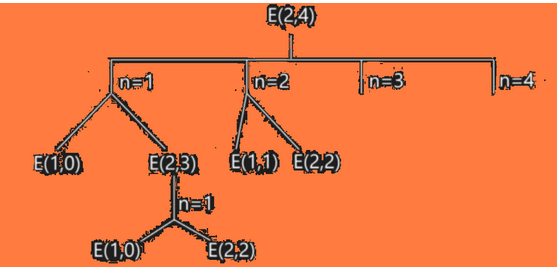
\includegraphics[width =11cm]{qESBw3q.png}    
\end{center}
In the above example E(1,0) and E(2,2) are processed two times.\\
Below is the code for the recursive approach\\
\newline
\begin{lstlisting}

#include <bits/stdc++.h> 
using namespace std; 

int max(int a, int b) 
{ 
    return (a > b) ? a : b; 
} 

int eggDrop(int n, int k) 
{ 
    if (k == 1 || k == 0) 
        return k; 

    if (n == 1) 
        return k; 

    int min = INT_MAX, x, res; 


    for (x = 1; x <= k; x++) { 
        res = max( 
            eggDrop(n - 1, x - 1), 
            eggDrop(n, k - x)); 
        if (res < min) 
            min = res; 
    } 

    return min + 1; 
} 

int main() 
{ 
    int n = 2, k = 10; 
    cout << "Minimum number of trials "
            "in worst case with "
        << n << " eggs and " << k 
        << " floors is "
        << eggDrop(n, k) << endl; 
    return 0; 
} 

\end{lstlisting}
But using the Dp we can easily reduce the time complexity.\\
Lets visualise this approach with an example . Lets find the optimum number of trials required for a 6 floored building and 3 eggs. Here E represents eggs and F represents floors.\\
\newline
\begin{center}
    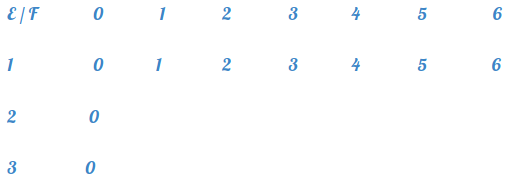
\includegraphics[width =11cm]{Yg7syDs.png}    
\end{center}
By using the below formula we can easily fill the table.\\
eggDrop(e,n) = 1+min{max( eggDrop(e-1,k-1) , eggDrop(e,n-k) ) , k in 1:n}\\
\begin{center}
    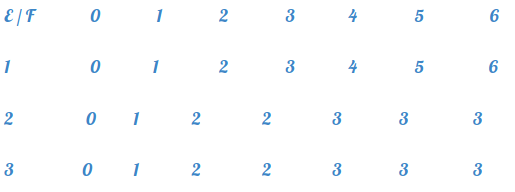
\includegraphics[width =11cm]{QVcKFnk.png}    
\end{center}
The code for the DP approach is below : - \\
\newline
\begin{lstlisting}
#include <limits.h> 
#include <stdio.h> 
int max(int a, int b) 
{ 
    return (a > b) ? a : b; 
} 

int eggDrop(int n, int k) 
{ 
    int eggFloor[n + 1][k + 1]; 
    int res; 
    int i, j, x; 

    for (i = 1; i <= n; i++) { 
        eggFloor[i][1] = 1; 
        eggFloor[i][0] = 0; 
    } 

    for (j = 1; j <= k; j++) 
        eggFloor[1][j] = j; 

    for (i = 2; i <= n; i++) { 
        for (j = 2; j <= k; j++) { 
            eggFloor[i][j] = INT_MAX; 
            for (x = 1; x <= j; x++) { 
                res = 1 + max( 
                            eggFloor[i - 1][x - 1], 
                            eggFloor[i][j - x]); 
                if (res < eggFloor[i][j]) 
                    eggFloor[i][j] = res; 
            } 
        } 
    } 


    return eggFloor[n][k]; 
} 


int main() 
{ 
    int n = 2, k = 36; 
    printf("\nMinimum number of trials "
        "in worst case with %d eggs and "
        "%d floors is %d \n", 
        n, k, eggDrop(n, k)); 
    return 0; 
} 

\end{lstlisting}

\chapter{Optimal Strategy for a Game}
\textbf{Problem Statement :-} In this we are given a row of n coins of values v1,...vn where n is even. Here n is even because the game is of two players and each plays equal no. of turns. The game we play against an opponent by alternating turns. The rule of the game is simple that a player selects either the first or last coin from the row of n coins. And we have to determine the maximum possible amount of money we can win if we are given to play the first move.\\
\newline
The best of this game is that the opponent is as clever as the player.\\
\newline
Lets understand this with an example .\\
Let there be a row of coins with values - \{3,9,1,2\}.\\
Now one approach (Greedy approach) that seems to be true is that choosing the best at each move gives an optimal solution . But is this right? No it is not right .\\
\newline
In the example according to the greedy approach the player will first choose 3 , then the opponent will choose 9 then the player will choose 2 and the opponent will\\
Finally choose 1.\\
Sum of the player coin values = 3 + 2 = 5.\\
And for the opponent the sum = 9 + 1 = 10.\\
\newline
But if we choose the non greedy approach the maximum value can be collected although the first move is not the best.\\
\newline
In this, approach the player will first choose 2 then the opponent will chose 3 then the player will chose 9 and the opponent will finally chose 1. Thus,\\
Sum of the player coin values = 9 + 2 = 11.\\
And for the opponent the sum = 3 + 1 = 4.\\
\newline
So we see clearly although we have not selected the maximum value in the first move, the resultant sum is the best(as both players are equally strong).\\
\newline
Approach to solve the problem.\\
As we know that both the players are equally strong both will try to reduce the possibility of the winning of each other. There can be two possibilities (considering the first value to chose in the array is at ith position and the last is at the jth position)-:\\
\textbf{1$>$} : The player chooses the ‘ith’ coin with value ‘vi’. Then the opponent have two options to chose (i+1)th or jth coin and he will chose in such a way that the player get the minimum value . Thus the player will collect the value vi + min(F(i+2,j),F(i+1,j-1)).\\
Here F(i, j) = max(vi, vj). \\
\textbf{2$>$} :  The user chooses ‘jth’ coin with value ‘vj’. The opponent either chooses ‘ith’ coin or ‘(j-1)th’ coin and he chooses in such a way that the player get the minimum value . Thus in this case the player will collect the value\\
Vj + min(F(i+1,j-1),F(i,j - 2)).\\
Since the player wants to maximize the number of coins we will chose the maximum of the above two cases. \\
\newline
Hence the final formula for the game will be.\\
\newline
F(i, j) = Max(vi + min(F(i+2,j),F(i+1,j-1)), Vj + min(F(i+1,j-1),F(i,j - 2))).\\
\newline
Code for this is given below.\\
\begin{lstlisting}
#include <bits/stdc++.h> 
using namespace std; 
int optimalStrategyOfGame( 
    int* arr, int n) 
{ 
    int table[n][n]; 

    for (int gap = 0; gap < n; ++gap) { 
        for (int i = 0, j = gap; j < n; ++i, ++j) { 
            int x = ((i + 2) <= j) 
                        ? table[i + 2][j] 
                        : 0; 
            int y = ((i + 1) <= (j - 1)) 
                        ? table[i + 1][j - 1] 
                        : 0; 
            int z = (i <= (j - 2)) 
                        ? table[i][j - 2] 
                        : 0; 

            table[i][j] = max( 
                arr[i] + min(x, y), 
                arr[j] + min(y, z)); 
        } 
    } 

    return table[0][n - 1]; 
} 

int main() 
{ 
    int arr1[] = { 8, 15, 3, 7 }; 
    int n = sizeof(arr1) / sizeof(arr1[0]); 
    printf("%d\n", 
        optimalStrategyOfGame(arr1, n)); 

    int arr2[] = { 2, 2, 2, 2 }; 
    n = sizeof(arr2) / sizeof(arr2[0]); 
    printf("%d\n", 
        optimalStrategyOfGame(arr2, n)); 

    int arr3[] = { 20, 30, 2, 2, 2, 10 }; 
    n = sizeof(arr3) / sizeof(arr3[0]); 
    printf("%d\n", 
        optimalStrategyOfGame(arr3, n)); 

    return 0; 
}

\end{lstlisting}
\chapter{Kadane’s Algorithm(Maximum Subarray Problem)}
Kadane’s algorithm - Given an array, the algorithm to find the maximum subarray sum is called kadane's algorithm.\\
\newline
Problem statement - The maximum subarray problem is the task of finding the largest possible sum of a contiguous subarray, with a given one - dimensional array A[1...n] of numbers.\\
\newline
Let’s consider an array A = \{-2, 1, -3, 4, -1, 2, 1, -5, 4\}.\\
\newline
We can see that largest possible sum of contiguous subarray of the above array is 6, which is of \{4, -1, 2, 1\}.\\
\newline
We will understand how we get to this result later.\\
\newline
First approach to solve is the brute force approach in this we calculate the sum of each of the subarray and then find the maximum of them. But you might notice that this is not a very good approach because as the size increases the number of possible subarrays increases rapidly, thus increases computational complexity. The time complexity by this method will be of $O(n^2)$ which is not very good.\\
\newline
Now we will see kadane’s algorithm to solve this problem.\\
Now let’s write all subarray ending with A[4] = -1 and A[5] =2.\\
Firstly we will write subarray ending with A[4] = -1.\\
\begin{center}
    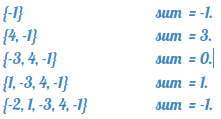
\includegraphics[width =8cm]{HJvIqJn.png}    
\end{center}
So the maximum here we find is 3. Similarly if we do with A[5] = 2, we will get that the maximum is 5. Now what if we know that the maximum till A[4] , we don’t need to compute for all the subarray for ending with A[5] we will only need to check those subarrays whose sum till A[4]is 3 and the single A[5] subarray and this leads to Kadane’s algorithm.\\
\newline
localmaximum[i] = max(A[i], A[i] + localmaximum[i - 1])\\
And the max of localmaximum[i] is equal to the largest possible sum of the contiguous subarray.\\
To calculate this we also use the fact that localmaximum[0] would be A[0] itself.\\
\newline
So using the above we can solve the problem in O(n).\\
\newline
Solving the above example by kadane’s algorithm.\\
\newline
\begin{lstlisting}
local_maximum[0] = -2.
local_maximum[1] = max(A[1], A[1] + local_maximum[0]) = max(1, - 1) = 1.
local_maximum[2] = max(A[2], A[2] + local_maximum[1]) = max(-3, -2) = -2.
Similarly 
local_maximum[3]  = 4.
local_maximum[4] = 3.
local_maximum[5] = 5.
local_maximum[6] = 6.
local_maximum[7] = 1.
local_maximum[8] = 5.

\end{lstlisting}
Thus the answer is 6.\\
\newline
Code for kadane’s algorithm is given below\\
\newline
\begin{lstlisting}
#include<bits/stdc++.h>
using namespace std;
int maxSubArraySum(int a[], int size)
{
int local_maximum[size + 1];
local_maximum[0] = a[0];

for (int i = 1; i < size; i++)
{
                local_maximum[i] = max(a[i], a[i] + local_maximum[i-1]);
}
int max_so_far = *max_element(local_maximum, local_maximum + size);
return max_so_far;
}

int main()
{
int a[] = {-2, -3, 4, -1, -2, 1, 5, -3};
int n = sizeof(a)/sizeof(a[0]);
int max_sum = maxSubArraySum(a, n);
cout << "Maximum contiguous sum is " << max_sum;
return 0;
}

\end{lstlisting}

\chapter{Calculating the sum of the elements of a sub-matrix in constant time}

Problem Statement - Given  a m * n matrix and two coordinates (p, q) and (r, s) which represents top -left and bottom -right coordinates of a sub-matrix of the given matrix, calculate the sum of all elements in the sub-matrix.\\
\newline
\begin{lstlisting}
Here 0 <= p < r < m and 0 <= 1 < s < n.
For example if we take the below matrix as input :-
[0 2 5 4 1]
[4 8 2 3 7]
[6 3 4 6 2]
[7 3 1 8 3]
[1 5 7 9 4]
 
In the above example taking
(p,q) = (1,1)
and (r, s) = (3, 3)

Then the output will be 38.

Now the explanation for this is too simple. The sub matrix formed by co ordinates (p, q),(p, s), (r, q) and (r, s) shown below having sum of elements equal to 38.

[8 2 3 ]
[3 4 6]
[3 1 8]

Assuming that m such lookup calls are made to the matrix, the task is to achieve O(1) time lookups.
The idea is to pre-process the matrix. We take an auxiliary matrix sum[][] where sum[i][j] will store the sum of the elements in matrix from (0,0) to (i,j). We can easily calculate the value of sum[i][j] in constant time using below relation -

Sum[i][j] = sum[i][j - 1] + sum[i - 1][j] + mat[i][j] - sum[i - 1][ j - 1];

Now the total sum can be calculated (of the matrix formed by the given coordinates) can be directly found by applying the below formula -
Total_sum =sum[r][s] - sum[r][q - 1] - sum[p - 1][s] + sum[p - 1][q - 1];

The code for this is given below -


#include <iostream>
using namespace std;

#define M 5
#define N 5

int findSubmatrixSum(int mat[M][N], int p, int q, int r, int s)
{
    int sum[M][N];

    sum[0][0] = mat[0][0];

    // pre-process first row
    for (int j = 1; j < N; j++)
        sum[0][j] = mat[0][j] + sum[0][j - 1];

    for (int i = 1; i < M; i++)
        sum[i][0] = mat[i][0] + sum[i - 1][0];
    for (int i = 1; i < M; i++)
    {
        for (int j = 1; j < N; j++)
        {
            sum[i][j] = mat[i][j] + sum[i - 1][j] + sum[i][j - 1]
                - sum[i - 1][j - 1];
        }
    }

    int total = sum[r][s];

    if (q - 1 >= 0)
        total -= sum[r][q - 1];

    if (p - 1 >= 0)
        total -= sum[p - 1][s];

    if (p - 1 >= 0 && q - 1 >= 0)
        total += sum[p - 1][q - 1];

    return total;
}

int main()
{
    int mat[M][N] =
    {
        { 0, 2, 5, 4, 1 },
        { 4, 8, 2, 3, 7 },
        { 6, 3, 4, 6, 2 },
        { 7, 3, 1, 8, 3 },
        { 1, 5, 7, 9, 4 }
    };

    int p = 1, q = 1, r = 3, s = 3;

    cout << findSubmatrixSum(mat, p, q, r, s);

    return 0;
}
\end{lstlisting}

\chapter{Maximum Sum Submatrix of size k $\times$ k in a given matrix n $\times$ n}

\textbf{\textit{Problem Statement:-}}\\
A $N \times N$ matrix is given, with all entries as integers. The task is to find the maximum sum of the subarray of size $k \times k$.\\

The simple solution is to consider all possible sub-squares of size $k \times k$ in our input matrix and then find the one which has maximum sum. Time complexity of above solution is $O(n^2 \cdot k^2)$.\\
As we can see that if we go to the above approach the time complexity is too big. We can solve this problem in $O(n^2)$ time. The idea behind this problem is to preprocess the given square matrix. In the preprocessing step, we will calculate the sum of all vertical strips of size $k \times 1$ in a temporary square matrix $stripSum$[ ][ ]. Once we have sum of all vertical strips, we can calculate sum of first sub-square in a row as sum of first k strips in that row, and for remaining sub-squares, we can calculate sum in $O(1)$ time by removing the leftmost strip of previous subsquare and adding the rightmost strip of new square.\\

The code for this is given below.

\begin{lstlisting}
#include <bits/stdc++.h> 
using namespace std; 

#define N 5 

void printMaxSumSub(int mat[][N], int k) 
{ 
	if (k > N) return; 
	int stripSum[N][N]; 

	for (int j=0; j<N; j++) 
	{ 
	    int sum = 0; 
		for (int i=0; i<k; i++) 
			sum += mat[i][j]; 
		stripSum[0][j] = sum; 

		for (int i=1; i<N-k+1; i++) 
		{ 
			sum += (mat[i+k-1][j] - mat[i-1][j]); 
			stripSum[i][j] = sum; 
		} 
	} 

	int max_sum = INT_MIN, *pos = NULL; 

	for (int i=0; i<N-k+1; i++) 
	{ 
		int sum = 0; 
		for (int j = 0; j<k; j++) 
			sum += stripSum[i][j]; 

		if (sum > max_sum) 
		{ 
			max_sum = sum; 
			pos = &(mat[i][0]); 
		} 
		for (int j=1; j<N-k+1; j++) 
		{ 
			sum += (stripSum[i][j+k-1] - stripSum[i][j-1]); 
			if (sum > max_sum) 
			{ 
				max_sum = sum; 
				pos = &(mat[i][j]); 
			} 
		} 
	} 

	for (int i=0; i<k; i++) 
	{ 
		for (int j=0; j<k; j++) 
			cout << *(pos + i*N + j) << " "; 
		cout << endl; 
	} 
} 

int main() 
{ 
	int mat[N][N] = {{1, 1, 1, 1, 1}, 
		{2, 2, 2, 2, 2}, 
		{3, 8, 6, 7, 3}, 
		{4, 4, 4, 4, 4}, 
		{5, 5, 5, 5, 5}, 
	}; 
	int k = 3; 

	cout << "Maximum sum 3 x 3 matrix is\n"; 
	printMaxSumSub(mat, k); 

	return 0; 
} 
\end{lstlisting}

\chapter{Count of different ways to express N as the sum of 1, 3 and 4}

In this algorithm we just represent N in the terms of (sum of ) 1’s ,3’s and 4’s. And count the possibilities of doing this. We divide problems into subproblems and solve them.\newline
And we also consider the order of integers. First define the $DP[n]$ array. Let it be the number of way to write $N$ as the sum of 1,3 and 4.\\
Consider one possible solution with $n = x_1 + x_2 + x_3 + … + x_n$.\newline
If the last number is 1, then sum of the remaining numbers is $n-1$. So the number that ends with 1 is equal to $DP[n-1]$. Taking other cases into account where the last number is 3 and 4.
The final recurrence would be:\\
\[DP_n = DP_{n-1} + DP_{n-3} + DP_{n-4}\]\\

\underline{Base Case :}
\begin{align*}
DP[0] &= 1\\
DP[1] &= 1\\
DP[2] &= 1\\
DP[3] &= 2\\
\end{align*}
	
\underline{Example:}\\
	N=4\newline
	Solutions: 4 $\mathtt{\{ 1+1+1+1 , 1+3 , 3+1 , 4 \}}$\newline
	
	N=6\newline
	Solutions : 6 $\mathtt{\{ 1+1+1+1+1 , 1+4 , 4+1 , 1+1+3 , 1+3+1 , 3+1+1 \}}$\\

\underline{Pseudo Code:}\\
\begin{lstlisting}
int countWays(int n)
{
	int DP[n+1];
	
	//base case
	DP[0]=1, DP[1]=1, DP[2]=1, DP[3]=2;
	
	//using iteration method for 4 to n

	for(int i=4; i<=n; i++)
	{
		DP[i] = DP[i-1] + DP[i-3] + DP[i-4];
	}
	return DP[n];
}
\end{lstlisting}

\underline{\\Time Complexity:}  $O(n)$\newline

\underline{Space Complexity:}  $O(n)$\newline


\chapter{Count of N digit numbers whose sum of digits equals to given sum}
In this approach we know how to find the total number whose digit sum is equal to the given sum and its total digit is equal to the given number.\\
Given: number of digit $N$, and sum of digits $sum$.\\

\underline{Example:}\\

1) $N = 2$ and $sum = 3$\\
$\mathbf{ans = 3 \{12,21,30\}}$\\

	
2) $N = 3$ and $sum = 6$\\
$\mathbf{ans = 21}$\\
$\mathbf{\{105, 114, 123, 132, 141, 150, 204,}$\\
$\mathbf{213, 222, 231, 240, 303, 312, 321,}$\\
$\mathbf{ 330, 402, 411, 420, 501, 510, 600\}}$\\

A simple solution would be to generate all $N$-digit numbers and count or print numbers that have sum of their digits equal to $sum$. The complexity of this solution would be exponential.\\

A better solution is to generate only those $N$-digit numbers that satisfy the given constraints. The idea is to use recursion. We basically fill all digit from 0 to 9 into current position and maintain sum of digits so far. We then perform recursion for remaining sum and number of digits left. We handle leading 0’s separately as they are not counted as digits.\\

\underline{Code:}\\
\begin{lstlisting}
#include <bits/stdc++.h>
using namespace std;
unsigned long long int countRec(int n, int sum)
{
     if (n == 0)
    return sum == 0;
    if (sum == 0)
    return 1;
    unsigned long long int ans = 0;
    for (int i=0; i<=9; i++)
    if (sum-i >= 0)
        ans += countRec(n-1, sum-i);
  
    return ans;
}
unsigned long long int finalCount(int n, int sum)
{
       unsigned long long int ans = 0;
      for (int i = 1; i <= 9; i++)
    if (sum-i >= 0)
        ans += countRec(n-1, sum-i);
      return ans;
}
int main()
{
    int n = 2, sum = 5;
    cout << finalCount(n, sum);
    return 0;
}
\end{lstlisting}


\textbf{\underline{Recursive Method:}}\\
\begin{lstlisting}
#include<bits/stdc++.h>
using namespace std;
unsigned long long int countRec(int n, int sum)
{
    if (n == 0)
        return sum == 0;
    if (lookup[n][sum] != -1)
        return lookup[n][sum];
    unsigned long long int ans = 0;
    for (int i=0; i<10; i++)
        if (sum-i >= 0)
            ans += countRec(n-1, sum-i);
    return lookup[n][sum] = ans;
}

unsigned long long int finalCount(int n, int sum)
{
    memset(lookup, -1, sizeof lookup);
    unsigned long long int ans = 0;
    for (int i = 1; i <= 9; i++)
        if (sum-i >= 0)
            ans += countRec(n-1, sum-i);
    return ans;
}

int main()
{
    int n = 3, sum = 5;
    cout << finalCount(n, sum);
    return 0;
}
\end{lstlisting}


\textbf{\underline{Another Method:}}\\

We can easily count $n$ digit numbers whose sum of digit equals to given sum by iterating all $n$ digits and checking if current $n$ digit number’s sum is equal to given sum, if it is then we will start increment number by 9 until it reaches to number whose sum of digit’s is greater than given sum, then again we will increment by 1 until we found another number with given sum.\\

\underline{Pseudo Code:}\\
\begin{lstlisting}
void findCount(int n, int sum) { 
    //in case n = 2 start is 10 and end is (100-1) = 99 
 int start = pow(10, n-1); 
 int end = pow(10, n)-1; 
    int count = 0; 
    int i = start; 
    while(i <= end) { 
       int cur = 0; 
       int temp = i; 
       while( temp != 0) { 
           cur += temp % 10; 
           temp = temp / 10; 
       } 
       if(cur == sum) {          	
           count++;          	
           i += 9;      	
       }
       else
           i++; 
    }  	
    cout << count;
} 
\end{lstlisting}

\underline{\\Time Complexity:}  $O(sum)$\newline

\underline{Space Complexity:}  $O(1)$\newline

\chapter{Remove array end element to maximize the sum of product:}
In this algorithm we remove array end element and maximize the sum of the product. We are allowed to remove element from either of the two side. We can remove element from the left side or right side. By using this opportunities we have to find the maximum sum of product.\\
We have a array of $N$ positive integers. Each time remove an element then score increased by\newline
\textit{(value of element) $\times$ (number of element already removed + 1)}.\newline\\
The task is to find the maximum score that can be obtained by removing all element.\\

\underline{Example:}\\

arr[ ] = $\mathbf{\{ 1, 3, 1 , 5, 2 \}}$\\
\textbf{Output: 43}
\newline
\newline
Remove 1 from left side (score = 1 $\times$ 1 = 1)\\
Then remove 2, (score = 1 + 2 $\times$ 2 = 5)\\
Then remove 3, (score = 5 + 3 $\times$ 3 = 14)\\
Then remove 1, (score = 14 + 1 $\times$ 4 = 18)\\
Then remove 5, (score = 18 + 5 $\times$ 5 = 43).\\

If Arr[ ]= $\mathbf{\{ 1, 2 \}}$\\
\textbf{Output: 5}
\newline
\newline
Remove 1 from left side (score = 1 $\times$ 1 = 1)\\
Then remove 2, (score = 1 + 2 $\times$ 2 = 5).\\

We use dynamic programming. First declare a 2D matrix named $dp$[ ][ ] initialised with 0, where $dp[i][j]$ denote the maximum value of score from index $i$ to $j$ of the array. So our final result will be stored in $dp[0][n-1]$.\\
We go for both possibilities by remove an element from left side or right side. Because our aim is find maximum. So value of $dp[i][j]$ will be\\
MAX($arr[i]$ $\times$ (\textit{number of element already removed + 1}) + $dp[i+ 1][j]$, $arr[j]$ $\times$ (\textit{number of element already removed + 1}) + $dp[i][j – 1]$.\\

\textbf{NOTE:}  If we sort array and apply this method then we find maximum output which can be or not can be output by upper approach (without sorting).\\

\underline{Pseudo Code:}\\

\begin{lstlisting}
int solve(int dp[][], int a[],int low,int high, int turn)
{
	//low is left side index and high is right side index.
	if(low == high)
		return a[low]*turn;
	if(dp[low][high] != 0)
		return dp[low][high];
	
	return dp[low][high] = 
	    max(
	    a[low]*turn + solve(dp,a,low + 1, high , turn +1), 
	    a[high]*turn + solve(dp, a, low, high - 1, turn + 1)
	    );

}
\end{lstlisting}

\underline{\\Time Complexity:}  $O(2^n)$\newline

\underline{Space Complexity:}  $O(n^2)$\newline

\chapter{Maximum subsequence sum such that no three are consecutive}
In this process we find the sum of subsequences and try to maximise it in given array. We are not  doing changes in the array. And the size of subsequences is 1 or 2 because we are not taking consecutive 3 elements from a given array. This is a restriction during doing this process.\\
Actually we use divide and conquer method to find solution. If $n = 1$ then sum is same of array, $n = 2$, $sum$ = sum of array’s elements. For $n > 2$, we use recursion method.\\

\underline{Example:}\\
arr[ ] = $\mathtt{\{ 1, 2, 3 \}}$\\
\textbf{Output: 5}
\newline
\newline
We can pick only two element from the array, so ans is 2 + 3 = 5\\

arr[ ] = $\mathtt{\{ 1, 2, 3, 4, 5, 6, 7, 8 \}}$\\
\textbf{Output: 27}
\newline
\newline
We take (7+8), (4+5) ,(2+1). So ans is 27.\\

\underline{Pseudo Code:}\\

\begin{lstlisting}
int maxsum(int arr[],int n)
{
    int sum[n];
    //Base cases
    if(n >= 1)
        sum[0] = arr[0];
    if(n >= 2)
        sum[1] = arr[0]+ arr[1];
    if(n > 2)
        sum[2] =
        max(sum[1], max(arr[1] + arr[2], arr[0] + arr[2]));

    for(int i=3 ; i<n ; i++)
        sum[i] =
        max(
        max( sum[i-1] , sum[i-2] + arr[i] ),
            arr[i] + arr[i-1] + sum[i-3]
        );
	
    return sum[n-1];
}
\end{lstlisting}

\textbf{\textit{Explanation:}}\\
	$sum[i]$ : Store the result for subarray $arr[0...i]$. This is the maximum possible sum in subarray $arr[0...i]$ such that no three elements are consecutive.\\
	
We have total 3 cases in general:
\newline
\newline
Exclude $arr[i]$ $\implies$ $sum[i] = sum[i-1]$
\newline
\newline
Exclude $arr[i-1]$ $\implies$ $sum[i] = sum[i-2] + arr[i]$
\newline
\newline
Exclude $arr[i-2]$ $\implies$ $sum[i-3] + arr[i] + arr[i-1]$
\newline
\newline
$sum[i]$ = max( $sum[i-1]$, $sum[i-2]$ + $arr[i]$, $sum[i-3]$ + $arr[i]$ + $arr[i-1]$)\\
	
By this 3 steps we proceed the above process.\\

\underline{Another Pseudo Code(using recursion):}

\begin{lstlisting}
int sum[1000000]; // and set to -1 to whole array
int maxsum(int arr[],int n)
{
    if(sum[n] != -1)
        return sum[n];
    if(n == 0)
        return sum[n] = 0;
    if(n == 1)	
        return arr[0];
    if(n == 2)
        return sum[n] = arr[1] + arr[0];

	return sum[n] = 
	max(
	    max(
	        maxsum(arr,n-1),maxsum(arr,n-2) + arr[n-1]
	       ),
	    arr[n-2] + arr[n-1] + maxsum(arr,n-3)
	);
}
\end{lstlisting}


\underline{\\Time Complexity:}  $O(n)$\newline

\underline{Space Complexity:}  $O(n)$\newline

\chapter{Maximum Subsequence Sum such that no k Elements are Consecutive}
In this process we find the sum of subsequences and try to maximise it for given array. We are not making changes in the array. The size of subsequences can be 1 to $k-1$ because we are not taking consecutive $k$ elements from a given array. This is a restriction during doing this process. We do this by using dynamic programming.\newline

Example :\newline
Input : arr[ ] = $\mathtt{\{ 10, 5, 8, 16, 21\}}$ \& $k = 4$\newline
	\textbf{Output: 55}\newline 
		Subsequences are $\mathtt{\{ 10\}}$, $\mathtt{\{ 8, 16, 21\}}$\newline\newline
Input: arr[ ] = $\mathtt{\{ 4, 12, 22, 18, 34, 12, 25\}}$\newline
	\textbf{Output: 111}\newline 
		Subsequences are $\mathtt{\{ 12, 22, 18, 34\}}$, $\mathtt{\{ 25\}}$\newline\newline

\underline{Pseudo Code:}\newline
\begin{lstlisting}
int max_sum(int arr[], int k,int n)
{
	int dp[n+1];
	memset(dp,0,n+1);
	int prefix[n+1];
	perfix[0]=0;
	for(int i=1;i<=n;i++)
		prefix[i]=perfix[i-1] + arr[i-1];

	dp[0]=0;
	for(int i=1;i<k;i++)
		dp[i]=prefix[i];

	for(int i=k;i<=n;i++)
	{
		for(int j=i;j>=(i-k+1);j--)
		{
			dp[i]=max(dp[i],dp[j-1] + prefix[i] -prefix[j]);
		}
	}

	return dp[n];
}
\end{lstlisting}
\textbf{\textit{Explanation:}}\newline\newline
First declare $dp$[ ] to memoize the maximum value of the sum up to each index.\newline
$dp[i]$ = max sum that can be picked such that no $k$ elements are consecutive from $0^{th}$ index to till $i^{th}$ index.\newline
\underline{Case $i < k$:}\newline  
If all element are positive then pick all the element before $K^{th}$ index.\newline
So $dp[1] = arr[0]$ , $dp[i] = dp[i-1] + arr[i-1]$.\newline\newline
\underline{Case $i \geq k$:}\newline 
We have to skip 1 element from $i$ to $(i-k+1)$ inclusive so to make sure that no $k$ elements are consecutive.\newline
Every element can contribute to the result so we skip every element which is lie with index $i$ to $(i-k+1)$ inclusive. If we skip $j^{th}$ element then max sum till $(j-1)^{th}$ index is given by $dp[j-1]$ with the sum of all the elements from $(j + 1)^{th}$ index to $i^{th}$ index .\newline\newline
Therefore update the current $dp$ state as:\newline$dp[i] = max (dp[i], dp[j -1] + prefix[i] – prefix [j]), (i \leq j \leq (i – K + 1))$\newline, where prefix array stores the prefix sum.\newline\newline
\underline{Time Complexity:} $O(n \cdot k)$\newline\newline
\underline{Space Complexity:} $O(n)$\newline\newline

\chapter{Unique Paths in a Grid with Obstacles}

\textbf{\textit{Problem statement:}}\newline
Given a grid to size $m\times n$ ,let us assume we are starting at (1,1) and our goal is to reach $(m, n)$,at any instant,if we are at $(x,y)$ we can either go to $(x,y+1)$ or $(x+1,y)$\\

Now consider if some obstacles are added to the grids. How many unique paths would be there?\newline
An obstacle and empty space are marked as 1 and 0.
\newline
\newline
An example is given below:\newline
Input:\newline
[[0,0,0],\newline
[0,1,0],\newline
[0,0,0]]\newline
\newline
\textbf{Output : 2}\newline
(As there is only one obstacle in the middle, we have two paths to reach )\newline
Using the naive recursive approach will result in exponential time complexity.\newline
\newline
The most efficient solution to this problem is by using dynamic programming. Like every dynamic programming concept we will not recompute the subproblems multiple times. A temporary 2D matrix will be constructed and value will be stored using the bottom up approach\\

Following is the approach to solve this problem:\\
i) We first create a 2-D matrix of the same size of the matrix to store the results.\newline
ii) We traverse through the array row wise and will start filling the values in it.\newline
iii) If an obstacle is found we set the value to 0\newline
iv) For the first row and column,we set the value to 1 if obstacle is not found\newline
v) For all remaining positions apart from the first row and first column and set the sum of right and upper values if obstacle is not present at that corresponding position in the given matrix.\newline
vi) We obtain the last value of the created 2d matrix.\newline

\underline{Pseudocode:}\\

\begin{lstlisting}
int main()
{
    int m,n
    cin>>m>>n
    int val[m+5][n+5],path[m+5][n+5] 
    for(int i=0;i<m;i++)
    {
        for(int j=0;j<n;j++)
        {
            cin>>val[i][j]
            path[i][j] = 0 /* initializing all values of 2d matrix path to 0 */
        }
    }
	//initializing the left corner if no obstacle is there
    if(val[0][0] == 0 )
    {
        Path[0][0] = 1
    }
	//initializing the first column of 2d matrix
    for(int i=1;i<m;i++)
    {
	   //if no obstacle is there in current cell
        if (vall[i][0] == 0)
        {
            path[i][0] = path[i-1][0]
        }
    }
      //initializing the first row of 2d matrix
    for(int i=1;i<n;i++)
    {
        //if no obstacle is there in current cell
        if (val[0][i] == 0)
        {
            path[0][i] = path[0][i-1]
        }
    }
    for(int i=1;i<m;i++)
    {
        for(int j=1;j<n;j++)
        {
            //if current cell is not an obstacle
            if(val[i][j]=0)
            {
                path[i][j] = path[i-1][j] + path[i][j-1]
            }
        }
    }
    //Corner value is the answer
    cout<<path[m-1][n-1]<<'\n';
    
    return 0;
}
\end{lstlisting}

\underline{Time Complexity:}\newline
We see that two nested for loops are being used,hence time complexity is $O(n^2)$\\

\underline{Space Complexity:}\newline
We see that 2-d arrays are being used ,therefore space complexity is $O(n^2)$\\
	
\chapter{Counting Number of Ways to reach $N^{th}$ Stair using Step 1, 2, 3}

\textbf{\textit{Problem Statement:}}\\

A child is running up a staircase with $n$ steps and can hop either 1 step, 2 steps or 3 steps at a time. Implement a method to count how many possible ways the child can run up the stairs.\\

Following are some examples:\newline
Input : 4\newline 
\textbf{Output : 7}\newline
\newline
Below are the number of ways in which the child can climb 4 stairs\newline
\begin{center}
1 step + 1 step + 1 step + 1 step\newline
1 step + 2 step + 1 step\newline
2 step + 1 step + 1 step\newline
1 step + 1 step + 2 step\newline
2 step + 2 step\newline
3 step + 1 step\newline
1 step + 2 step\newline
\end{center}

Input : 3\newline 
\textbf{Output : 4}\newline
\newline
Below are the number of ways in which the child can climb 3 stairs\newline
\begin{center}
1 step + 1 step + 1 step\newline
1 step + 2 step\newline
2 step + 1 step\newline
3 step\newline
\end{center}

There are 2 methods to solve this problem\newline
We first see the naive recursive approach and then we will see a much faster dynamic programming solution.\\

\textbf{\textit{Recurxive Approach:}}\\
Given there are $n$ stairs and a person is allowed to jump next stair, skip one stair or skip two stairs. Therefore if a person is standing at $i^{th}$ stair, he can move to $i+1^{th}$, $i+2^{th}$ or $i+3^{th}$ stair. Hence a recursive function can be formed where if current index is $i$,to reach stair $i$, a person can jump either from $i-1^{th}$, $i-2^{th}$, $i-3^{th}$ stair or $i^{th}$ is the starting stair.\\
We now look at the recursive function\newline
\newline
step(i) = step(i-1) + step(i-2) + step(i-3)\newline
(step(i) is the number of ways to reach i-th stair)\\

Base case will at n=1,n=1 and n=2 for n=1 and n=0 step(i) = 1 and for n=2 step(i) = 2\\

\underline{Pseudocode:}\\

\begin{lstlisting}
//this function returns number of ways to reach a stair n
int step(int n)
{
    //base cases
    if (n == 1 || n == 0)
        return 1;
    else if (n == 2)
        return 2;
    else  //recursive part 
        return
        step(n-1) + step (n-2) + step(n-3);
}
int main()
{
    int n;
    cin>>n;
    cout<<step(n)<<'\n;
    return 0;
}
\end{lstlisting}

\underline{Time complexity:}\\
The time complexity of the above solution is exponential, a close upper bound will be $O(3^n)$. From each state, 3 recursive function are called. So the upperbound for $n$ states is $O(3^n)$.\\

\underline{Space Complexity:} $O(1)$.\newline
As no extra space is required.\\

\textbf{\textit{Working of the recursive function:}}\\

We now look at the dynamic programming approach\newline\newline
\textit{Dynamic Programming approach:}\\
The method of dynamic programming is similar to that of the recursive approach. It is observed that in recursive approach some states are called repeatedly. So the idea is to store the value of states. This thing can be done in two ways:\newline\newline
\textbf{i) Top-Down Approach:} In this approach we keep the recursive structure intact and just store the value in a HashMap and whenever the function is called again we return the value without computing it.\newline\newline
\textbf{ii) Bottom-Up Approach:} The second way is to take an extra space of size $n$ and start computing values of states from 1,2.. to n,i.e compute values of $i$, $i+1$, $i+2$ and then use them to calculate the value of $i+3$.\newline\newline
Following is the steps of the algorithm:\newline\newline
1) Create an array of size $n+1$ and initialize base cases,these are first 3 variables with 1,1,2\newline.
2) Run a loop from 3 to $n$.\newline
3) For each index $i$,compute the value of $i^{th}$ position as dp[i]  = dp[i-1] + dp[i-2] + dp[i-3]\newline
4) Print the value of dp[n], which is the number of ways to reach the $n^{th}$ step.\newline\newline
\underline{Pseudocode:}\\

\begin{lstlisting}
int main()
{
    int n;
    cin>>n;
    int res[n+5]
    //initializing the base cases
    res[0]=1;
    res[1]=1;
    res[2]=2;
       //dp part
    for(int i=3;i<n;i++)
    {
        res[i] = res[i-1] + res[i-2] + res[i-3];
    }
    cout<<res[n]<<'\n; //This prints number of ways
    return 0;
}
\end{lstlisting}

\underline{Time complexity:}\\
As one for loop is being used the time complexity is $O(n)$\\

\underline{Space complexity:}\\
Due to usage of an array,the space complexity is $O(n)$\\

\chapter{Count Balanced Binary Trees of Height $h$}

\textbf{\textit{Problem statement:}}\\

Given a height $h$, count the maximum number of balanced binary trees possible with the given height.\newline
What is a balanced binary tree?\newline
A balanced binary tree is one in which for every node, the difference between heights of left and right subtree is not more than one.\newline\newline
Following are the balanced binary trees of height 3.
\newline
\begin{center}
    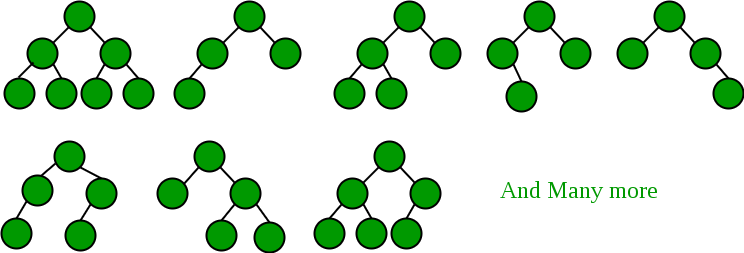
\includegraphics[width = 10cm]{Balanced_Binary_Tree-1.png}    
\end{center}
Height of tree, \textit{h = 1 + max(left height, right height)}\newline
We know that the difference between the height of left and right subtree is not more than one, therefore the possible heights of left and right can be one of the following:\newline
\begin{center}
(h-1),(h-2)\newline
(h-2),(h-1)\newline
(h-1),(h-1)\newline    
\end{center}

    We see that we now get the following recursive formula
\begin{align*}
count(h) &= count(h-1)\times count(h-2) + count(h-2)\times count(h-1) + count(h-1)\times count(h-1)\\
&=2\times count(h-1)\times count(h-2) + count(h-1)\times count(h-1)\\
&= count(h-1)\times(2\times count(h-2) + count(h-1))\newline
\end{align*}
From the above we can see that the problem is having the optimal substructure property.
We now see the naive recursive method to solve this problem\newline\newline
Here binarytreecount(int h) is a function to count no of balanced tree.\newline

\begin{lstlisting}
int binarytreecount(int h)
{
    //only one tree is possible with height 0 or 1
    //this is the base case
    if(h == 0 || h == 1)
    return 1;
    return 
    binarytreecount(h-1)*(2*binarytreecount(h-2) + binarytreecount(h-1));
}
\end{lstlisting}

We see that the time complexity of this approach is exponential\newline
The recursion tree with $h = 3$ looks as the following\newline\newline

\begin{center}
    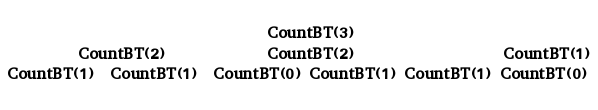
\includegraphics[width = 10cm]{Balanced_Binary_Tree-2.png}    
\end{center}

\textbf{\textit{Dynamic Programming approach:}}\\
As we can observe, sub-problems are being solved repeatedly therefore we store the results as we compute them.\\

\underline{Pseudo code:}\\

\begin{lstlisting}
int main()
{
    int h;
    cin>>h;
    int dp[h+5];
      //we set up base cases
    dp[0]=1;
    dp[1]=1;
    for(int i=2;i<=h; i++)
    {
        dp[i] = (dp[i - 1] * ((2 * dp [i - 2]);
    }
    /*this calculates total number of balanced binary trees of height h */
    cout<<dp[h]<<'\n;
    return 0;
}
\end{lstlisting}

\underline{Time complexity:}\\
Since we are using a for loop ,the time complexity is $O(n)$\\

\underline{Space complexity:}\\
Since we are using an array,space complexity is $O(n)$\\

\chapter{Finding Number of Solutions of a Linear Equation of $\textbf{\textit{n}}$ Variables}

\textbf{\textit{Problem Statement:}}\\
Given a linear equation of $n$ variables, find the number of non-negative solutions of it. For example, let the equation be “x+2 y=5”,solutions of this equation are “x=1,y=2”,”x=5,y=0” and ”x=3,y=1”. It may be assumed that all coefficients in given equation are positive integers.\newline\newline
Following are some examples:\newline\newline
Input: coeff[] = $\mathtt{\{1, 2\}}$, rhs = 5\newline
\textbf{Output: 3}\newline\newline
The equation $x + 2y = 5$ has 3 solutions.\newline
(x=1,y=1), (x=1,y=2), and (x=5,y=0)\newline

Input: coeff[] = $\mathtt{\{2, 2, 3\}}$, rhs = 4\newline
\textbf{Output: 3}\newline\newline
The equation $2x + 2y + 2z = 4$ has 3 solutions.\newline
(x=0, y=2, z=0),(x=2, y=0, z=0), and (x=1, y=1, z=0)\newline
\newline
We first look at the naive recursive solution of this problem.\newline\newline
\textbf{\textit{Recursive solution:}}\\
The idea in recursive approach is to subtract first coefficient from rhs and then recur for remaining value of rhs.\newline\newline
Following is the recursive function countsol\newline

\begin{lstlisting}[mathescape]
if rhs = 0 
    countsol(coeff, 0, rhs, n-1) = 1
else 
    countsol(coeff, 0, rhs, n-1) = $\Sigma$countSol(coeff, i, rhs-coeff[i], m-1) 
where coeff[i] <= rhs and i varies from 0 to n-1
\end{lstlisting}

\underline{Pseudocode for recursive approach:}\\
\newline
\begin{lstlisting}
int numsol(int coeff[],int start,int end,int rhs)
{
    //This is the base case
    if (rhs == 0)
    return 1
    /* we now initialize the count of the solutions*/
    int ans = 0
    /*one by one we are subtracting all smaller or equal coefficients and then recurring.*/
    for (int i=start;i<=end;i++)
    {
        if (coeff[i]<= rhs)
        {
            ans+=numsol(coeff,i,end,rhs-coeff[i])
        }
    }
    return ans
}

int main()
{
    int n,rhs;
    cin>>n>>rs;
	int coeff[n+5];
    for(int i=0;i<n;i++)
    {
        cin>>coeff[i]
    }
    cout<<numsol(coeff,0,n-1,rhs)
}
\end{lstlisting}

We see that since we are using a recursive function, we are getting an exponential time complexity. This can be solved in Pseudo Polynomial time complexity using Dynamic Programming. From recursive solution we can see it is having optimal substructure and overlapping subproblems, therefore we can use dynamic programming.\newline\newline

\textbf{\textit{Dynamic Programming Approach:}}\\

We are storing all the values in an array dp and we are storing result of subproblems in it.\\

\underline{Pseudocode:}\\
\begin{lstlisting}
int main()
{
int rhs, n;
cin>>n>>rhs;
int dp[n+5], coeff[n+5];
/*creating and initializing a table to store results of subproblems*/
for(int i=0; i<n; i++)
{
    cin>>coeff[i];
    dp[i]=0;
}
//filling the table in bottom up manner
for (int i=0; i<n; i++)
{
    for(int j=coeff[i];j<=rhs;j++)
    {
        dp[j] += dp[j-coeff[i]];
    }
}
    cout<<dp[rhs];
    return 0;
}
\end{lstlisting}

\underline{Time complexity:}\\
We see that two nested are being used here therefore time complexity is $O(n \times rhs)$\\

\underline{Space complexity:}\\
We see are using arrays therefore space complexity is $O(n)$.\\


\part{Application of dynamic programming}
 
 \newpage
 .\large{  \\ \\ \\ \\ \\ \\ \\ \\ \\ \\
	We have understood what dynamic programming is and how useful it is to solve varies problems. In this section we highlight some applications and real life examples of dynamic programming.\\\\ \\\\	}
 \newpage
 \chapter{Introduction}
  Let us take a real life example. We all know how google map works in real life, but on looking deeper you can see that it is designed on dynamic programming algorithms. How do they work?\\\\
 Let's try to understand by making an assumption that world consists of 10 cities and they are connected by some roads. If we assume that cities are nodes and roads are edges, we get a graph. Moreover, if you want to find the distance from one city to another city you can use Dijkstra's algorithm, Bellman Ford (uses dynamic programming) or Floyd Warshall (uses dynamic programming). We already discussed these algorithms in previous sections.\\\\
  \textbf{\textit{Now we discuss real-world application of dynamic programming}}\newline\newline
(1).\underline{
\textbf{Image process:}}\\
 Image process is using orthogonal algorithm. This algorithm is based on the search of the transformation that brings the second image over first image and minimizes the L1 and L2 distance. The matching is global and does not require any previous segmentation or feature extraction.\\
 dynamic programming is used in the orthogonal algorithm because it appeared to be the most efficient way for performing an optimal strip to strip matching. 
\\\\
(2).\underline{
\textbf{Bioinformatics:}}\\
The most significant application is in field of bioinformatics. they are used in the sequence alignment and in the protein folding.
they are helpful in RNA structure prediction and in the DNA binding.\\
First dynamic programming algorithms for protein-DNA binding were developed in the 1970s independently by Charles Delisi in USA and Georgi Gurskii and Alexanderr zasedatelev in USSR.
\\\\
(3).\underline{
\textbf{Database:}}\\
Dynamic programming is the time honored method for optimizing join queries in relational database management systems and virtually all commercial optimizer rely on some abbreviated form of DP for this purpose.dynamic programming  uses  exhaustive enumeration with pruning to produce “optimal” execution plans without missing the best of these plans. dynamic programming also used for dedicated cachetiers storing data to avoid database access.
\\\\
(4).\underline{
\textbf{Webserver for biological sequence alignment:}}\\
Scanning genome and protein sequence databases is an essential task in molecular biology.Biologists find out the structural  and  functional  similarities  between  a  query  sequence and a subject database sequence by scanning the existing  genome  or  protein  database  sequences,  with  real  world applications in disease diagnosis, drug engineering, bio-material engineering and genetic engineering of plants and  animals.  There  are  numbers  of  biological  sequence  alignment       algorithms       with       various       execution       speed/accuracy  tradeoffs.  Among  these,  we  cite  dynamic  programming   based   algorithms.\\
The  Needleman-Wunsch  (NW)  and  Smith-Waterman  (SW)    algorithms    are    two    widely    used    dynamic    programming algorithms for pairwise biological sequence alignment.   Needleman-Wunsch   is   a   global   alignment   algorithm,  which  is  suitable  for  small  sequences,  as  it  aligns the sequences from the beginning to the end. In the case  of  longer  sequences,  Needleman-Wunsch  introduces  too  much  gap  penalty  noises  that  reduce  the  accuracy  of  the  alignment.
\\\\
(5).\underline{
\textbf{Operating system:}}\\
dynamic programming use for the prevent fetching the same data multiple times and save CPU cycles by avoiding recomputation.it is use for time sharing to design operating system.which was use for schedules the job to maximize CPU usage.
\\\\
(6).\underline{
\textbf{Water Resoureces system:}}\\
The dynamic programming optimization techniques have been extensively used in water resources.The major reason dynamic programming is so attractive for these problems is the great generality of the problem formulation to which it can be applied. Non-linearities in the system equations and performance criterion can easily be handled. Constraints on both decision and state variables introduce no difficulties. Stochastic effects can be explicitly taken into account.
\\\\
(7). \underline{
\textbf{Connected speech Recognition}}\\
In a system of speech recognition containing words, the recognition requires the comparison between the entry signal of the word and the various words of the dictionary. The 
problem can be solved efficiently by a dynamic comparison algorithm whose goal is to put in 
optimal correspondence the temporal scales of the two words. An algorithm of this type is 
Dynamic Time Warping. This paper presents two alternatives for implementation of the algorithm designed for recognition of the isolated words. 
\\\\
(8). \underline{
\textbf{Slope statbility:}}\\
The applicability of the dynamic programming method to two-dimensional slope stability analyses is studied. The critical slip surface is defined as the slip surface that yields the minimum value of an optimal function. The only assumption regarding the shape of the critical slip surface is that the surface is an assemblage of linear segments. Stresses acting along the critical slip surface are computed using a finite element stress analysis. Assumptions associated with limit equilibrium methods of slices related to the shape of the critical slip surface and the relationship between interslice forces are no longer required.\\ A computer program named DYNPROG was developed based on the proposed analytical procedure, and numerous example problems have been analyzed. Results obtained when using DYNPROG were compared with those obtained when using several well-known limit equilibrium methods. The comparisons demonstrate that the dynamic programming method provides a superior solution when compared with conventional limit equilibrium methods.
\\\\
(9).\underline{
\textbf{Decision making:}}\\
In large warehouses, box packing with minimal cost. Ever wondered how Amazon uses algorithms to decide which product should go into which cardboard box. The decision to use effecient resources is many a times, knapsack decision. also for game stragery we can use dynamic programming or greedy to know best result.
\\\\ 
Some of use of dynamic programming is for git merge ,shipment routing in ecommerce websites is very lkikely modelled as shorest path algorithm,knuth's word wrapping algorithm,in computer chess the use of transposition tables and refutation tables,viterbi algorithm used for hidden markov models,the earley algorithm,dynamic time wrapping, De Boor algorithm,Duckworth lewis method this is used of resolving the problem when games of cricket are interrupted, markov decision processes,some methods for solving interval schedulling problems,beat traking in music information retrievel,Adaptive-critic training strategy for artificial neural networks,Stereo algorithms for solving the correspondence problem used in stereo vision,Seam carving (content-aware image resizing),Optimization of electric generation expansion plans in the Wein Automatic System Planning (WASP).

\end{document}
